\documentclass[12pt,a4paper]{jarticle} % pLaTeX
%%% LaTeXパッケージのインクルード %%%
\usepackage[cpp,ja]{fdps-tutorial} % チュートリアル文書用スタイルファイル
\usepackage{udline}

%%% udline の設定 %%%
%\newcommand{\uwave}[1]{{\setnami\uc{#1}}}
\newcommand{\usaw}[1]{{\setnoko\uc{#1}}}

% タイトル、著者、作成日の情報
\title{\docTitle}
\author{谷川衝}
\author{行方大輔}
\author{細野七月}
\author{岩澤全規}
\author{似鳥啓吾}
\author{村主崇行}
\author{野村昴太郎}
\author{牧野淳一郎}
\affil{\affiliation}
\date{}


% 文書の開始
\begin{document}

% タイトルと目次の出力
\maketitle
\tableofcontents

\clearpage

%%%%%%%%%%%%%%%%%%%%%%%%%%%%%%%%%%%%%%%%%%%%%%%%%%%%%
\section{変更記録}
\label{sec:changelog}
\begin{itemize}
\item 2015.03.13
  \begin{itemize}
  \item Correct \texttt{getRsearch} to \texttt{getRSearch}. (section
    \ref{sec:userdefined}).
  \item Add a function \texttt{PS::Abort} (section \ref{sec:initfin}).
  \end{itemize}
\item 2015.03.17
  \begin{itemize}
  \item Release version 1.0
  \end{itemize}
\item 2015.03.18
  \begin{itemize}
  \item Modify the licence related to class Particle Mesh.
  \end{itemize}
\item 2015.03.20
  \begin{itemize}
  \item Add the description of \texttt{PS::Comm::broadcast}.
  \end{itemize}
\item 2015.04.01
  \begin{itemize}
  \item Add a caution that class Particle Mesh does not work in the
    case of 1 MPI process.
  \end{itemize}
  \item 2015.10.07
  \begin{itemize}
  \item Add the description of PM method. Section
    \ref{sec:module_extended_PM}。
  \end{itemize}
\item 2015.12.01
  \begin{itemize}
  \item Add the description of Multiwalk method. Sections
    \ref{sec:example_userdefined_calcForceDispatch}、
    \ref{sec:example_userdefined_calcForceRetrieve}、
    \ref{sec:module_standard_treeforforce_calcforceallandwriteback}、
    \ref{sec:userdefined_calcForceDispatch}、
    \ref{sec:userdefined_calcForceRetrieve}。
  \end{itemize}
\item 2016.02.19
  \begin{itemize}
  \item Added descriptions for \texttt{getNeighborListOneParticle} in 
    \ref{sec:neighborlist}.

  \item In accordance with the above change, added the descriptions of 
    \texttt{PS:: MomentMonopoleScatter} and
    \texttt{PS::MomentQuadrupoleScatter} in 
    section  \ref{sec:MomentForSearchModeLong}.

  \item Added the descriptions of their wrappers,
    \texttt{MonopoleWithScatter} 
    and 
    \texttt{QuadrupoleWithScatter},
    to section  \ref{sec:module_treeforce_standard_search_mode_long}.

  \end{itemize}


  \item 2016.09.13
  \begin{itemize}
  \item Added APIs for removing or adding particles. The discription
    of them is added in \ref{sec:addAndRemoveParticle}.
  \item The discription of out-of-range access in type Vector is added
    in section \ref{sec:errormessage:vector_invalid_access}.
  \end{itemize}

    \item 2016.10.11
  \begin{itemize}
  \item The implementation of the operator ``[]'' in the Vector class
    is cahnged. Added remarks of the Vector class in section \ref{sec:datatype_vector}.
  \end{itemize}

  \item 2016.11.04
  \begin{itemize}
  \item Added APIs for IO in sections
    \ref{sec:readParticleAscii},\ref{sec:readParticleBinary},\ref{sec:writeParticleAscii},\ref{sec:writeParticleBinary}.
  \end{itemize}

    \item 2017.07.11
  \begin{itemize}
  \item Added a discription about reusing interaction list in section
    \ref{sec:treeForForceHighLevelAPI}.
  \end{itemize}

    \item 2017.09.06
  \begin{itemize}
  \item Added API for sorting FP in particle system. The discription of this API is in section
    \ref{sec:ParticleSystem:sortParticle}.
  \item Added API for obtaining a pointer of EPJ from its id. The
    discription of this API is in section
    \ref{sec:EPJ:getId},\ref{sec:getEpjFromId}.
  \end{itemize}

    \item 2017.11.08
  \begin{itemize}
  \item Release FDPS version 4.0.
  \end{itemize}

  \item 2018.01.16
    \begin{itemize}
    \item Release FDPS version 4.0b.
      \begin{itemize}
      \item Fix a bug for memory allocation.
      \item Add destructors for TreeForForce class, etc.
      \end{itemize}
    \end{itemize}

  \item 2018.01.23
    \begin{itemize}
    \item Descriptions for APIs of the serialization of particle data in exchange of particles are added in Sections \ref{sec:FP:serialize}, \ref{sec:EPJ:serialize}, \ref{sec:SPJ:serialize},          \ref{sec:particleSystem:exchangeParticle}, and \ref{sec:treeForForceHighLevelAPI} (\textcolor{red}{specification only; not yet implemented}).
    \end{itemize}

  \item 2018.05.25
    \begin{itemize}
    \item Release FDPS version 4.0c.
      \begin{itemize}
      \item MPI C++ bindings in Particle Mesh extension are eliminated.
      \end{itemize}
    \end{itemize}

  \item 2018.06.13
    \begin{itemize}
    \item Release FDPS version 4.1.
      \begin{itemize}
      \item Fix an issue when $\theta=0$ is specified (FDPS makes superparticles in some situations).
      \item Description of orthotope type is added in Section \ref{sec:datatype_orthotope}.
      \item Description of required member functions for specific cases is added in Section of Moment class.
      \end{itemize}
    \end{itemize}

  \item 2018.06.20
    \begin{itemize}
    \item Release FDPS version 4.1a.
      \begin{itemize}
      \item Fix an omission in this section.
      \end{itemize}
    \end{itemize}

  \item 2018.08.2
    \begin{itemize}
    \item A new API \texttt{getBoundaryCondition} is added.
    \item The meaning of the argument \texttt{weight} of API \texttt{collectSampleParticle} is described in detail.
    \end{itemize}

  \item 2018.12.7
    \begin{itemize}
    \item Release FDPS version 5.0a.
       \begin{itemize}
          \item Descriptions on pre-defined classes for \newline
          \texttt{PS::SEARCH\_MODE\_LONG\_SCATTER} \newline
          \texttt{PS::SEARCH\_MODE\_LONG\_SYMMETRY} \newline
          are added to the sections of Moment and SuperParticleJ classes (\S~\ref{sec:moment} and \S~\ref{sec:superparticlej}).
          \item Descriptions on member functions \texttt{readBinary} and \texttt{writeBinary} are added to the sections of FullParticle and header classes (\S~\ref{sec:fullparticle} and \S~\ref{sec:userdefined_header}). Examples of implementations of them are also added to \S~\ref{sec:example_fullparticle} and \S~\ref{sec:example_userdefined_header}.
       \end{itemize}
    \end{itemize}

  \item 2018.12.9
    \begin{itemize}
    \item Release FDPS 5.0b.
       \begin{itemize}
          \item In accurate description of API \texttt{getNeighborListOneParticle} is fixed (No changes in the source codes of FDPS except for the version information).
       \end{itemize}
    \end{itemize}

  \item 2019.1.25
    \begin{itemize}
    \item Release FDPS 5.0c.
       \begin{itemize}
          \item A bug that causes an error in function LinkCell under certain conditions is fixed.
       \end{itemize}
    \end{itemize}

  \item 2019.3.1
    \begin{itemize}
    \item Release FDPS 5.0d.
       \begin{itemize}
          \item Fixed a bug that the size of root cell of a tree becomes too large for specific boundary conditions.
          \item Fixed a bug that member variables \texttt{make\_LET\_1st}, \texttt{make\_LET\_2nd}, \newline \texttt{exchange\_LET\_1st}, and  \texttt{exchange\_LET\_2nd} of class \texttt{PS::TimeProfile} are not correctly set for some \texttt{PS::SEARCH\_MODE} in FDPS version 5.0 - 5.0c. As we changed the scopes of time measurement, each value of these member variables is not compatible with that in FDPS version 4.1 or earlier, but the sum of them is compatible.
          \item Fixed a problem that user's code stops due to segmentation fault when the memory pool used inside FDPS runs out.
          \item This version of FDPS uses a feature of C++11. \textcolor{red}{Hence, users must add an appropriate compiler option such as \texttt{-std=c++11} in \texttt{gcc} to your C++ and CUDA compilers.}
       \end{itemize}
    \end{itemize}
    
  \item 2019.3.7
    \begin{itemize}
    \item Improved the description on TreeForForLong$\langle$,,$\rangle$::MonopoleWithCutoff.
    \end{itemize}

  \item 2019.9.6
    \begin{itemize}
    \item Release FDPS 5.0f
       \begin{itemize}
          \item Fixed a problem that triggers a compile error when compiling with option \texttt{-DPARTICLE\_SIMULATOR\_TWO\_DIMENSION}.
       \end{itemize}
    \end{itemize}

  \item 2019.9.10
    \begin{itemize}
    \item Release FDPS 5.0g
       \begin{itemize}
          \item Fixed a problem that triggers a runtime error when compiling with option \texttt{-DPARTICLE\_SIMULATOR\_TWO\_DIMENSION}.
       \end{itemize}
    \end{itemize}

  \item 2020.8.16
    \begin{itemize}
    \item Release FDPS 6.0
       \begin{itemize}
          \item PIKG (\url{https://github.com/FDPS/PIKG}) included.
       \end{itemize}
    \end{itemize}
    
  \item 2020.8.18
    \begin{itemize}
    \item Release FDPS 6.0a
       \begin{itemize}
          \item The version of PIKG bundled is updated to v0.1b
       \end{itemize}
    \end{itemize}

  \item 2020.8.19
    \begin{itemize}
    \item Release FDPS 6.0b
       \begin{itemize}
          \item The implementations of the sample codes of $N$-body simulation in \path{sample/*/nbody} are improved so that they shows better performance when using kernels generated by PIKG.
       \end{itemize}
    \end{itemize}

\end{itemize}

\clearpage

%%%%%%%%%%%%%%%%%%%%%%%%%%%%%%%%%%%%%%%%%%%%%%%%%%%%%
\section{概要}
\label{sec:overview}
この節ではFDPSの概要を記述する。FDPSの開発目的、FDPSの基本的な考えかた、
FDPSを使用して作成したコードの動作について概説する。

%%%%%%%%%%%%%%%%%%%%%%%%%%%%%%%%%%%%%%%%%%%%%%%%%%%%%%%%%%%%%%%%%%%%%%
\subsection{開発目的}

粒子シミュレーションは、重力$N$体シミュレーション、SPHシミュレーション、
渦糸法、MPS法、分子動力学シミュレーションなど理学工学の様々な分野で使
用されている。より大きい空間スケール、より高い空間分解能(または質量分
解能)、より長い時間スケールの物理現象を追跡するために、高性能な粒子シ
ミュレーションコードへの要請はますます強くなっている。

高性能な粒子シミュレーションコードを組むためには、シミュレーションコー
ドの大規模並列化を避けることはできない。粒子シミュレーションコードの大
規模並列化をする際には、ロードバランスのため動的領域分割、領域分割に合
わせた粒子交換、ノード間通信の削減と最適化、キャッシュ利用効率の向上、
SIMDユニット利用効率の向上、アクセラレータへの対応など、数多くの困難な
処理を行う必要がある。現在、研究グループは個別にこれらの処理へ対応して
いる。

しかし、上記の処理は粒子シミュレーション共通のものである。FDPSの開発目
的は、これらの処理を高速に行うライブラリを提供し、大規模並列化への対応
に追われていた研究者の負担を軽くすることである。FDPSを使うことで、研究
者がよりクリエイティブな仕事に専念できるようになれば、幸いである。

%%%%%%%%%%%%%%%%%%%%%%%%%%%%%%%%%%%%%%%%%%%%%%%%%%%%%%%%%%%%%%%%%%%%%%
\subsection{基本的な考えかた}

ここではFDPSの基本的な考えかたについて記述する。

%%%%%%%%%%%%%%%%%%%%%%%%%%%%%%%%%%%%%%%%%%%%%%%%%%%%
\subsubsection{大規模並列粒子シミュレーションの手順}
\label{sec:overview_concept_abstraktion}

まずFDPSにおいて、大規模並列粒子シミュレーションがどのような手順で行わ
れることを想定しているかを記述する。粒子シミュレーションは、以下のよう
な微分方程式を時間発展させるものである。
\begin{align}
    \frac{d\bm{u}_i}{dt} = \sum_j f(\bm{u}_i,\bm{u}_j) + \sum_s
    g(\bm{u}_i,\bm{v}_s) \label{eq:GoverningEquation}
\end{align}
ここで$\bm{u}_i$は粒子$i$の物理量ベクトルであり、この物理量には質量、
位置、速度など粒子が持つあらゆる物理量が含まれる。関数$f$は粒子$j$から
粒子$i$への作用を規定する。以後、作用を受ける粒子を$i$粒子、作用を与え
る粒子を$j$粒子と呼ぶことにする。$\bm{v}_s$は$i$粒子から十分遠方にある
粒子を1つの粒子としてまとめた粒子(以後、この粒子を超粒子と呼ぶ)の物理
量ベクトルである。関数$g$は超粒子から$i$粒子への作用を規定する。式
(\ref{eq:GoverningEquation})の第2項は、重力やクーロン力など無限遠まで
到達する長距離力の場合はゼロではない。しかし流体の圧力のような短距離力
はゼロである。

大規模並列化された粒子シミュレーションコードは以下の手順で式
(\ref{eq:GoverningEquation})を時間発展させる。ここではデータの入出力や
初期化は省略している。
\begin{enumerate}
\item 以下の2段階の手順でどのプロセスがどの粒子の式
  (\ref{eq:GoverningEquation})を時間発展させるか決める。
  \label{item:LoadBalance}
  \begin{enumerate}
  \item プロセスの間でロードバランスを取れるように、シミュレーションで
    扱っている空間の領域を分割し、各プロセスの担当領域を決める(領域分
    割)。
  \item 各プロセスが、自分の担当する領域に存在する全粒子の物理量ベクト
    ル$\bm{u}_i$を持つように、他のプロセスと物理量ベクトル$\bm{u}_i$を
    交換する(粒子交換)。
  \end{enumerate}

\item 各プロセスは、自分の担当する全粒子の式
  (\ref{eq:GoverningEquation})の右辺を計算するのに必要な$j$粒子の物理
  量ベクトル$\bm{u}_j$と超粒子の物理量ベクトル$\bm{v}_s$を他のプロセス
  と通信することで集めて、$j$粒子のリストと超粒子のリスト(まとめて相互
  作用リストと呼ぶ)を作る(相互作用リストの作成)。
  \label{item:MakeInteractionList}

\item 各プロセスは自分の担当する全粒子に対して、式
  (\ref{eq:GoverningEquation})の右辺を計算し、$d\bm{u}_i/dt$を求める
  (相互作用の計算)。\label{item:CalcInteraction}

\item 各プロセスは、自分の担当する全粒子の物理量ベクトル$\bm{u}_i$とそ
  の時間導関数$d\bm{u}_i/dt$を使って、全粒子の時間積分を実行し、次の時
  刻の物理量ベクトル$\bm{u}_i$を求める(時間積分)。
  \label{item:IntegrateTime}

\item 手順\ref{item:LoadBalance}に戻る。        
\end{enumerate}

%%    ただし、あらゆる相互作用のタイプに対応するには以下5種類の$j$粒子
%%    と超粒子の集め方が必要。\label{item:MakeInteractionList}    
%%    \begin{itemize}
%%        \item 長距離力モード:$i$粒子に対して、近い粒子は$j$粒子として、
%%        遠方の複数の粒子はまとめて超粒子として集めるモード(使用例:開
%%        放条件下の重力やクーロン力)
%%        \item 長距離力モードカットオフ付き:長距離力モードとほぼ同じだ
%%        が、ある距離より遠い粒子は集めないモード(使用例:周期境界条件
%%        下の重力やクーロン力)
%%        \item 短距離力収集モード:$i$粒子自身の持つサーチ半径の内側に
%%        ある粒子のみ$j$粒子として集めるモード(使用例:SPH法における密
%%        度の計算)
%%        \item 短距離力散乱モード:$i$粒子をサーチ半径の内側に含む粒子
%%        を$j$粒子として集めるモード(使用例:Lennard-Jones力)
%%        \item 短距離力対称モード:短距離力収集モードで集める粒子と短距
%%        離力散乱モードで集める粒子の和集合を$j$粒子として集めるモード
%%        (使用例:SPH法における圧力勾配の計算)    
%%    \end{itemize}

%%%%%%%%%%%%%%%%%%%%%%%%%%%%%%%%%%%%%%%%%%%%%%%%%%%%
\subsubsection{ユーザーとFDPSの役割分担}

FDPSは、プロセス間の通信が発生する処理はFDPSが担当し、プロセス間の通信
の発生しない処理はユーザーが担当するという役割分担を基本としている。従っ
て、前節に挙げた、領域分割・粒子交換(項目\ref{item:LoadBalance})・相互
作用リストの作成(項目\ref{item:MakeInteractionList})をFDPSが、相互作用
の計算(項目\ref{item:CalcInteraction})・時間積分(項目
\ref{item:IntegrateTime})をユーザーが担当することになる。ユーザーは
FDPSのAPIを呼び出すだけで、大規模並列化に関わる煩雑な処理を避けつつ、
高性能な任意の相互作用の粒子シミュレーションコードを手に入れることがで
きる。

%%%%%%%%%%%%%%%%%%%%%%%%%%%%%%%%%%%%%%%%%%%%%%%%%%%%
\subsubsection{ユーザーのやること}

ユーザーがFDPSを使って粒子シミュレーションコードを作成するときにやるこ
とは以下の項目である。
\begin{itemize}

%%\item 座標系の選択(節\ref{sec:compile_coordinate})。2次元または3次元
%%  直角座標系の選択が可能。

%%\item 境界条件の選択(節\ref{sec:datatype_enum_boundarycondition})。開
%%  放境界条件、x, y, z軸方向どれかまたはすべての周期境界条件の選択が可
%%  能。
    
\item 粒子の定義(節\ref{sec:userdefined})。粒子の持つ物理量(式
  (\ref{eq:GoverningEquation})で言えば$\bm{u}_i$)の指定。例えば質量、
  位置、速度、加速度、元素組成、粒子サイズ、など。

\item 相互作用の定義(節\ref{sec:userdefined})。粒子間の相互作用(式
  (\ref{eq:GoverningEquation})で言えばで関数$f$, $g$)を指定。例えば、
  重力、クーロン力、圧力、など。

\item FDPSのAPIの呼出(節\ref{sec:initfin}, \ref{sec:module})

\end{itemize}

%%%%%%%%%%%%%%%%%%%%%%%%%%%%%%%%%%%%%%%%%%%%%%%%%%%%
\subsubsection{補足}

式(\ref{eq:GoverningEquation})の右辺は2粒子間相互作用の重ね合わせであ
る。従って、FDPSのAPIを呼ぶだけでは、3つ以上の粒子の間の相互作用の計算
を行うことはできない。しかし、FDPSはネイバーリストを返すAPIを用意して
いる。ネイバーリストを用いれば、ユーザーはプロセス間の通信の処理をする
ことなく、このような相互作用の計算をできる。

節\ref{sec:overview_concept_abstraktion}で示した手順は、全粒子が同じ時
間刻みを持っている。そのため、FDPSのAPIを呼び出すだけでは、独立時間刻
みで時間積分を効率的に行うことができない。しかし、上と同じくネイバーリ
ストを返すAPIがあるため、Particle Particle Particle Tree法を用いて独立
時間刻みを実装することは可能であろう。

%%マルチプロセス, マルチスレッド, SIMD演算を用いて, 並列に処理される.
%%FDPSはC++言語にて記述される.

%%%%%%%%%%%%%%%%%%%%%%%%%%%%%%%%%%%%%%%%%%%%%%%%%%%%%%%%%%%%%%%%%%%%%%
\subsection{コードの動作}
\label{sec:overview_action}

ここではFDPSを使用して作成したコードの動作の概略を記述する。このコード
には、4つのモジュールがあることになる。3つはFDPSのモジュールで、1つ
はユーザー定義のモジュールである。まとめると以下のようになる。
\begin{itemize}
\item 領域クラス:全プロセスが担当する領域の情報と、領域分割を行うAPI
  を持つ
\item 粒子群クラス:全粒子の情報と、プロセスの間での粒子交換を行うAPI
  を持つ
\item 相互作用ツリークラス:粒子分布から作られたツリー構造と、相互作用
  リストを作成するAPIを持つ
\item ユーザー定義クラス:ある1粒子を定義するクラス、粒子間の相互作用
  を定義する関数オブジェクトを持つ
\end{itemize}

これら4つのモジュールの間で情報がやり取りされる。これは図
\ref{fig:brief_interface}で概観できる。図\ref{fig:brief_interface}に示
された情報のやりとりは、節\ref{sec:overview_concept_abstraktion}に記述
された手順\ref{item:LoadBalance}から\ref{item:CalcInteraction}と、これ
らの手順以前に行われる手順(手順0とする)に対応する。
以下はこれらの手順の詳細な記述である。
\begin{enumerate}
\item[0.] ユーザー定義クラスのうち1粒子を定義するクラスが粒子群クラス
  へ、粒子間の相互作用を定義する関数オブジェクトが相互作用ツリークラス
  へ渡される。これはクラスの継承ではなく、粒子を定義するクラスは粒子群
  クラスのテンプレート引数として、粒子間の相互作用を定義する関数オブジェ
  クトは相互作用ツリークラスのAPIの引数として渡される
\item[\ref{item:LoadBalance}.] 以下の2段階でロードバランスを取る
  \begin{enumerate}
  \item 領域クラスが持つ領域分割のAPIが呼ばれる。このとき粒子情報が粒
    子群クラスから領域クラスへ渡される (赤字と赤矢印)
  \item 粒子群クラスが持つ粒子交換のAPIが呼ばれる。このとき領域情報が
    領域クラスから粒子群クラスへ渡される (青字と青矢印)
  \end{enumerate}
\item[\ref{item:MakeInteractionList}.] 相互作用ツリークラスが持つ相互
  作用リストを作成するAPIが呼ばれる。このとき領域情報が領域クラスから
  相互作用ツリークラスへ、粒子情報が粒子群クラスから相互作用ツリークラ
  スへ渡される (緑字と緑矢印)
\item[\ref{item:CalcInteraction}.] 相互作用ツリーククラスが持つ相互作
  用を定義した関数オブジェクトを呼び出すAPIが呼ばれる。相互作用計算が
  実行され、相互作用計算の結果が相互作用ツリークラスから粒子群クラスへ
  渡される (灰色の字と灰色矢印)
\end{enumerate}

%% ルートドメイン
%% ドメイン
%% リアル粒子
%% フル粒子
%% イメージ粒子
%% セル
%% リーフ

\begin{figure}[h]
  \begin{center}
    %    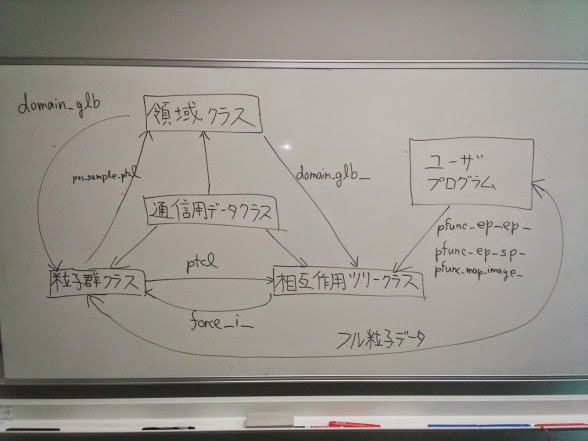
\includegraphics[width=10cm,bb=0 0 600 500]{fig/brief_interface.jpg}
    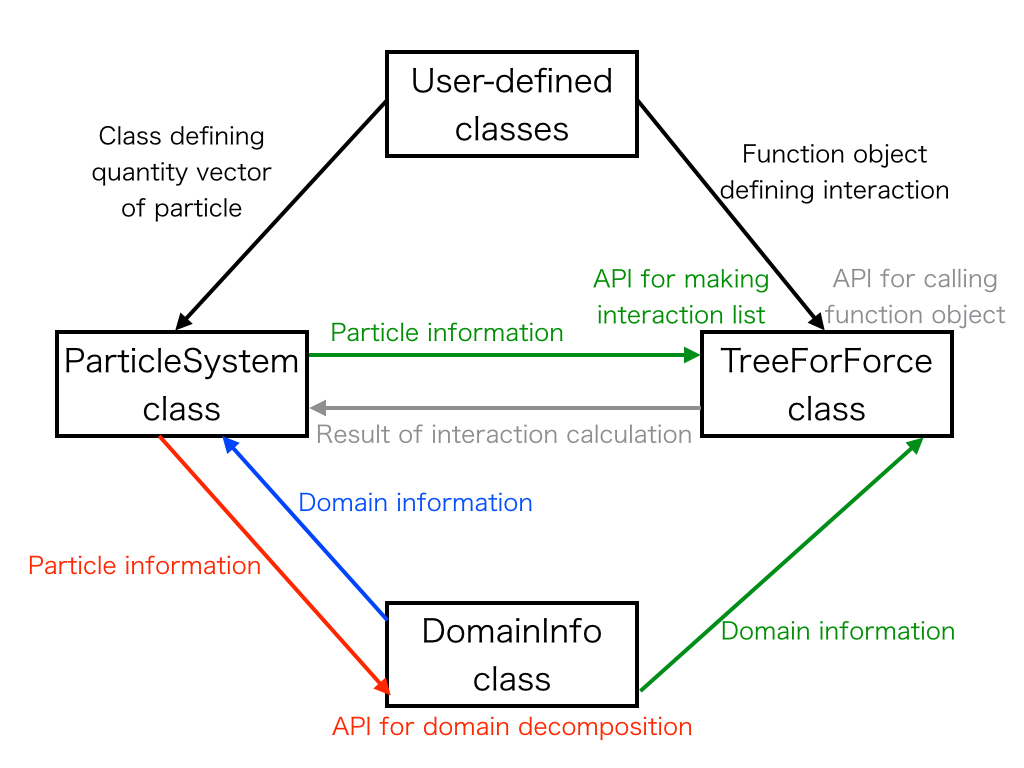
\includegraphics[width=10cm,bb=0 0 700 700]{fig/illustration/illustration.001.jpg}
  \end{center}
  \caption{モジュールインターフェースと情報の流れの模式図。}
  \label{fig:brief_interface}
\end{figure}

\clearpage

%%%%%%%%%%%%%%%%%%%%%%%%%%%%%%%%%%%%%%%%%%%%%%%%%%%%%
\section{入門:サンプルコードを動かしてみよう}
\label{sec:getting_started}
%================================
%   この節の概要/内容について
%================================
本節では、まずはじめに、FDPS\describeForEach{}{および FDPS Fortranインターフェース}{および FDPS C言語インターフェース}の動作環境、必要なソフトウェア、インストール方法などを説明し、その後、サンプルコードの使用方法を説明する。サンプルコードの中身に関しては、次節(第\ref{sec:how_to_use}節)で詳しく述べる。

%%%%%%%%%%%%%%%%%%%%%%%%%%%%%%%%%%%%%%%%%%%%%%%%%%%%%
\subsection{動作環境}
FDPSはLinux, Mac OS X, WindowsなどのOS上で動作する。

%%%%%%%%%%%%%%%%%%%%%%%%%%%%%%%%%%%%%%%%%%%%%%%%%%%%%
\subsection{必要なソフトウェア}
本節では、FDPSを使用する際に必要となるソフトウェアを記述する。まず標準
機能を用いるのに必要なソフトウェア、次に拡張機能を用いるのに必要なソフ
トウェアを記述する。
%%%%%%%%%%%%%%%%%%%%%%%%%%%%%%%
\subsubsection{標準機能}
本節では、FDPSの標準機能のみを使用する際に必要なソフトウェアを記述する。
最初に逐次処理機能のみを用いる場合(並列処理機能を用いない場合)に必要
なソフトウェアを記述する。次に並列処理機能を用いる場合に必要なソフトウェ
アを記述する。
%%%%%%%%%%%%%%%%
\subsubsubsection{逐次処理}
逐次処理の場合に必要なソフトウェアは以下の通りである。
\begin{itemize}
\item make
\item C++コンパイラ(gccバージョン4.8.3以降なら確実, Kコンパイラバージョ
  ン1.2.0で動作確認済)
\describeForFtn{% Fortran版記述[開始]
\item Fortranコンパイラ (Fortran 2003 標準をサポートし、上記 C++コンパイラと相互運用可能なもの。gcc 4.8.3 以降のgfortranなら確実)
\item Python 2.7.5以上、または、Python 3.4以上 (これ以外での正常動作は保証しない。特に、Python 2.7以前では動作しない)
}%Fortran版記述[終了]
\describeForC{% C言語版記述[開始]
\item Cコンパイラ (上記 C++コンパイラと相互運用可能なもの。gcc 4.8.3 以降のgfortranなら確実)
\item Python 2.7.5以上、または、Python 3.4以上 (これ以外での正常動作は保証しない。特に、Python 2.7以前では動作しない)
}%C言語版記述[終了]

\end{itemize}
%%%%%%%%%%%%%%%%
\subsubsubsection{並列処理}
本節では、FDPSの並列処理機能を用いる際に必要なソフトウェアを記述する。
まず、OpenMPを使用する際に必要なソフトウェア、次にMPIを使用する際に必要
なソフトウェア、最後にOpenMPとMPIを同時に使用する際に必要なソフトウェア
を記述する。
%%%%%%%%
\subsubsubsubsection{OpenMP}
OpenMPを使用する際に必要なソフトウェアは以下の通り。
\begin{itemize}
\item make
\item OpenMP対応のC++コンパイラ(gcc version 4.8.3以降なら確実, Kコンパ
  イラバージョン1.2.0で動作確認済)
\describeForFtn{% Fortran版記述[開始]
\item OpenMP対応のFortranコンパイラ (Fortran 2003 標準をサポートし、上記 C++コンパイラと相互運用可能なもの。gcc 4.8.3以降なら確実)
\item Python 2.7.5以上、または、Python 3.4以上 (これ以外での正常動作は保証しない。特に、Python 2.7以前では動作しない)
}%Fortran版記述[終了]
\describeForC{% C言語版記述[開始]
\item OpenMP対応のCコンパイラ (上記 C++コンパイラと相互運用可能なもの。gcc 4.8.3以降なら確実)
\item Python 2.7.5以上、または、Python 3.4以上 (これ以外での正常動作は保証しない。特に、Python 2.7以前では動作しない)
}%C言語版記述[終了]

\end{itemize}
%%%%%%%%
\subsubsubsubsection{MPI}
MPIを使用する際に必要なソフトウェアは以下の通り。
\begin{itemize}
\item make
\item MPI version 1.3対応のC++コンパイラ(Open MPI 1.6.4で動作確認済, K
  コンパイラバージョン1.2.0で動作確認済)
\describeForFtn{%Fortran版記述[開始]
\item MPI version 1.3対応のFortranコンパイラ (Fortran 2003 標準をサポートし、上記 C++コンパイラと相互運用可能なもの。Open MPI 1.6.4で動作確認済み)
\item Python 2.7.5以上、または、Python 3.4以上 (これ以外での正常動作は保証しない。特に、Python 2.7以前では動作しない)
}%Fortran版記述[終了]
\describeForC{%C言語版記述[開始]
\item MPI version 1.3対応のCコンパイラ (上記 C++コンパイラと相互運用可能なもの。Open MPI 1.6.4で動作確認済み)
\item Python 2.7.5以上、または、Python 3.4以上 (これ以外での正常動作は保証しない。特に、Python 2.7以前では動作しない)
}%C言語版記述[終了]

\end{itemize}
%%%%%%%%
\subsubsubsubsection{MPI+OpenMP}
MPIとOpenMPを同時に使用する際に必要なソフトウェアは以下の通り。
\begin{itemize}
\item make
\item MPI version 1.3とOpenMPに対応のC++コンパイラ(Open MPI 1.6.4で動
  作確認済, Kコンパイラバージョン1.2.0で動作確認済)
\describeForFtn{%Fortran版記述[開始]
\item MPI version 1.3とOpenMPに対応のFortranコンパイラ(Fortran 2003標準をサポートし、上記 C++コンパイラと相互運用可能なもの。Open MPI 1.6.4で動作確認ずみ)
\item Python 2.7.5以上、または、Python 3.4以上 (これ以外での正常動作は保証しない。特に、Python 2.7以前では動作しない)
}%Fortran版記述[終了]
\describeForC{%C言語版記述[開始]
\item MPI version 1.3とOpenMPに対応のCコンパイラ(上記 C++コンパイラと相互運用可能なもの。Open MPI 1.6.4で動作確認ずみ)
\item Python 2.7.5以上、または、Python 3.4以上 (これ以外での正常動作は保証しない。特に、Python 2.7以前では動作しない)
}%C言語版記述[終了]

\end{itemize}
%%%%%%%%%%%%%%%%%%%%%%%%%%%%%%%
\subsubsection{拡張機能}
本節では、FDPSの拡張機能を使用する際に必要なソフトウェアについて述べる。
FDPSの拡張機能にはParticle Meshがある。以下ではParticle Meshを使用する
際に必要なソフトウェアを述べる。
%%%%%%%%%%%%%%%%
\subsubsubsection{Particle Mesh}
Particle Meshを使用する際に必要なソフトウェアは以下の通りである。
\begin{itemize}
\item make
\item MPI version 1.3とOpenMPに対応のC++コンパイラ(Open MPI 1.6.4で動
  作確認済)
\item FFTW 3.3以降
\end{itemize}

%%%%%%%%%%%%%%%%%%%%%%%%%%%%%%%%%%%%%%%%%%%%%%%%%%%%%
\subsection{インストール}
本節では、FDPS\describeForEach{}{および FDPS Fortranインターフェース}{および C言語インターフェース}のインストールについて述べる。取得方法、ビルド方法について述べる。
%%%%%%%%%%%%%%%%%%%%%%%%%%%%%%%
\subsubsection{取得方法}
ここではFDPSの取得方法を述べる。最初に最新バージョンの取得方法、次に過去のバージョンの取得方法を述べる。
%%%%%%%%%%%%%%%%
\subsubsubsection{最新バージョン}
以下の方法のいずれかでFDPSの最新バージョンを取得できる。
\begin{itemize}
\item ブラウザから
  \begin{enumerate}
  \item ウェブサイト \url{https://github.com/FDPS/FDPS}で"Download ZIP"をクリックし、ファイル\path{FDPS-master.zip}をダウンロード
  \item FDPSを展開したいディレクトリに移動し、圧縮ファイルを展開
  \end{enumerate}

\item コマンドラインから
  \begin{itemize}    
  \item Subversionを用いる場合:以下のコマンドを実行するとディレクトリ
    trunkの下をSubversionレポジトリとして使用できる
    \begin{screen}
\begin{verbatim}
$ svn co --depth empty https://github.com/FDPS/FDPS
$ cd FDPS
$ svn up trunk
\end{verbatim}
    \end{screen}

  \item Gitを用いる場合:以下のコマンドを実行するとカレントディレクト
    リにディレクトリFDPSができ、その下をGitのレポジトリとして使用できる
    \begin{screen}
\begin{verbatim}
$ git clone git://github.com/FDPS/FDPS.git
\end{verbatim}
    \end{screen}    

  \end{itemize}

\end{itemize}
%%%%%%%%%%%%%%%%
\subsubsubsection{過去のバージョン}
以下の方法でブラウザからFDPSの過去のバージョンを取得できる。
\begin{itemize}
\item ウェブサイト\url{https://github.com/FDPS/FDPS/releases}に過去のバージョ
  ンが並んでいるので、ほしいバージョンをクリックし、ダウンロード
\item FDPSを展開したいディレクトリに移動し、圧縮ファイルを展開
\end{itemize}
\if 0
\begin{itemize}
\item ブラウザから
  \begin{enumerate}
  \item ウェブサイト \url{https://github.com/FDPS/FDPS/releases}に過去のバージョンが並んでいるので、ほしいバージョンをクリックし、ダウンロード
  \item FDPSを展開したいディレクトリに移動し、圧縮ファイルを展開
  \end{enumerate}

\item コマンドラインから
  \begin{itemize}
    
  \item Gitを用いる場合:以下のコマンドを実行するとカレントディレクト
    リにディレクトリFDPSができる。
    \begin{screen}
\begin{verbatim}
$ git clone git://github.com/FDPS/FDPS.git
\end{verbatim}
    \end{screen}

    ディレクトリFDPSに移動し、以下のコマンドを実行すると、存在するFDPS
    の過去のバージョンがわかる。以下では、v0.1, v0.2, v1.0というバージョ
    ンが存在していることになる。
    \begin{screen}
\begin{verbatim}
$ git tag
v0.1
v0.2
v1.0
\end{verbatim}
    \end{screen}

    以下のコマンドを実行すると、ダウンロードしたFDPSがv0.1バージョンに
    なっている。ここではブランチを切らない場合を示す。
    \begin{screen}     
\begin{verbatim}
$ git checkout refs/tags/v0.1
\end{verbatim}
    \end{screen}

  \end{itemize}

\end{itemize}
\fi
%%%%%%%%%%%%%%%%%%%%%%%%%%%%%%%
\subsubsection{インストール方法}
\describeForCpp{%C++版記述
\texttt{configure}などをする必要はない。
}
\ifIF %Fortran,C版記述
C++言語で記述されたFDPS本体はヘッダライブラリ\footnote{ヘッダファイルだけで構成されるライブラリのこと}のため、\texttt{configure}などを行う必要はない。基本的にはアーカイブを展開したあと、自分のソースファイルをコンパイルする時に適切なインクルードパスを設定すればよい。実際の手続きは第\ref{subsec:usage_of_sample_codes}節で説明するサンプルコードとその Makefile をみて欲しい。

\progLangName の場合、コンパイル前に \progLangName ソースファイルからFDPSとのインターフェースコードを生成する必要がある。その手順は仕様書\href{file://./doc_specs_ftn_ja.pdf}{doc\_spec\_ftn\_ja.pdf}の第6章に記述されている。本サンプルコードのMakefileでは、インターフェースコードが \texttt{make} コマンド実行中に自動的に生成されるようになっている。ユーザが自分のコードの Makefile を作る時にはサンプルコードの Makefile を参考にすることを推奨する。
\endifIF


%%%%%%%%%%%%%%%%%%%%%%%%%%%%%%%%%%%%%%%%%%%%%%%%%%%%%
\subsection{サンプルコードの使用方法}
\label{subsec:usage_of_sample_codes}
本節ではサンプルコードの使用方法について説明する。サンプルコードには重力$N$体シミュレーションコードと、SPHシミュレーションコードがある。最初に重力$N$体シミュレーションコード、次にSPHシミュレーションコードの使用について記述する。サンプルコードは拡張機能を使用していない。
%%%%%%%%%%%%%%%%%%%%%%%%%%%%%%%
\subsubsection{重力$N$体シミュレーションコード}
\label{subsubsec:usage_of_sample_codes:nbody}
本サンプルコードは、\describeForEach{FDPS}{FDPS Fortranインターフェース}{FDPS C言語インターフェース}を用いて書かれた無衝突系の$N$体計算コードである。このコードでは一様球のコールドコラプス問題を計算し、粒子分布のスナップショットを出力する。
%%%%%%%%%%%%%%%%
\subsubsubsection{概要}
以下の手順で本コードを使用できる。
\begin{itemize}
\item ディレクトリ\dirNameNbodySample に移動。これ以後、ディレクトリ\texttt{\$(FDPS)}はFDPSの最も上の階層のディレクトリを指す(\texttt{\$(FDPS)}は環境変数にはなっていない)。\texttt{\$(FDPS)}はFDPSの取得によって異なり、ブラウザからならFDPS-master, Subversionからならtrunk, GitからならFDPSである。
\item カレントディレクトリにある\texttt{Makefile}を編集
\item コマンドライン上で\texttt{make}を実行
\item \texttt{nbody.out} ファイルの実行
\item 結果の解析
\end{itemize}
最後にx86版Phantom-GRAPEおよびPIKGを使う場合について述べる。

%%%%%%%%%%%%%%%%
\subsubsubsection{ディレクトリ移動}
ディレクトリ\dirNameNbodySample に移動する。

%%%%%%%%%%%%%%%%
\subsubsubsection{Makefileの編集}
\label{s3sec:how_to_edit_Makefile_in_nbody}
\ifCpp%C++用
\texttt{Makefile}の編集項目は以下の通りである。OpenMPとMPIを使用するかどうかで編集方法が変ることに注意。
\endifCpp
\ifFtn%Fortran用
サンプルコードのディレクトリには2つのMakefileがある。1つはGCC用に書かれた\texttt{Makefile}であり、もう1つはIntelコンパイラ用に書かれた\texttt{Makefile.intel}である。ここでは\texttt{Makefile}について詳しく解説し、\texttt{Makefile.intel}に関しては使用上の注意点を本節最後で述べるのみとする。

まず、\texttt{Makefile}の初期設定について説明する。サンプルコードをコンパイルするにあたって、ユーザが設定すべきMakefile変数は4つあり、Fortranコンパイラを表す\texttt{FC}、C++コンパイラを表す\texttt{CXX}、それぞれのコンパイルオプションを表す\texttt{FCFLAGS}, \texttt{CXXFLAGS}である。これらの初期設定値は次のようになっている:
\begin{screen}
\begin{Verbatim}[commandchars=\\\{\}]
FC=gfortran
CXX=g++
FCFLAGS = -std=f2003 -O3 -ffast-math -funroll-loops -finline-functions
CXXFLAGS = -O3 -ffast-math -funroll-loops \$(FDPS_INC)
\end{Verbatim}
\end{screen}
ここで、\texttt{\$(FDPS\_INC)}はFDPS本体をインクルードするために必要なインクルードPATHが格納された変数であり、\texttt{Makefile}内で設定済みである。したがって、ここで変更する必要はない。

上記4つのMakefile変数の値を適切に編集し、\texttt{make}コマンドを実行することで実行ファイルが得られる。OpenMPとMPIを使用するかどうかで編集方法が変わるため、以下でそれを説明する。
\endifFtn
\ifC%C言語用
サンプルコードのディレクトリにはGCC用に書かれた\texttt{Makefile}がある。以下、この\texttt{Makefile}について解説する。

まず、\texttt{Makefile}の初期設定について説明する。サンプルコードをコンパイルするにあたって、ユーザが設定すべきMakefile変数は4つあり、Cコンパイラを表す\texttt{CC}、C++コンパイラを表す\texttt{CXX}、それぞれのコンパイルオプションを表す\texttt{CFLAGS}, \texttt{CXXFLAGS}である。これらの初期設定値は次のようになっている:
\begin{screen}
\begin{Verbatim}[commandchars=\\\{\}]
CC=gcc
CXX=g++
CFLAGS = -O3 -ffast-math -funroll-loops -finline-functions \$(FDPS_INC)
CXXFLAGS = -O3 -ffast-math -funroll-loops \$(FDPS_INC)
\end{Verbatim}
\end{screen}
ここで、\texttt{\$(FDPS\_INC)}はFDPS本体をインクルードするために必要なインクルードPATHが格納された変数であり、\texttt{Makefile}内で設定済みである。したがって、ここで変更する必要はない。

上記4つのMakefile変数の値を適切に編集し、\texttt{make}コマンドを実行することで実行ファイルが得られる。OpenMPとMPIを使用するかどうかで編集方法が変わるため、以下でそれを説明する。
\endifC

\begin{itemize}
%%% OpenMPもMPIも使用しない場合 %%%
\item OpenMPもMPIも使用しない場合
\begin{itemize}
\describeForEach{%C++用
\item 変数\texttt{CC}にC++コンパイラを代入する
}{%Fortran用
\item 変数\texttt{FC}にFortranコンパイラを代入する
\item 変数\texttt{CXX}にC++コンパイラを代入する
}{%C言語用
\item 変数\texttt{CC}にCコンパイラを代入する
\item 変数\texttt{CXX}にC++コンパイラを代入する
}
\end{itemize}
%%% OpenMPのみ使用の場合 %%%
\item OpenMPのみ使用の場合
\begin{itemize}
\describeForEach{%C++用
\item 変数\texttt{CC}にOpenMP対応のC++コンパイラを代入する
\item \texttt{CFLAGS += -DPARTICLE\_SIMULATOR\_THREAD\_PARALLEL -fopenmp}の行のコメントアウトを外す。Intelコンパイラの場合には、\texttt{-fopenmp}を\texttt{-qopenmp}か\texttt{-openmp}に変更する(どちらを指定すべきかはコンパイラのバージョンに依る)。
}{%Fortran用
\item 変数\texttt{FC}にOpenMP対応のFortranコンパイラを代入する
\item 変数\texttt{CXX}にOpenMP対応のC++コンパイラを代入する
\item \texttt{FCFLAGS += -DPARTICLE\_SIMULATOR\_THREAD\_PARALLEL -fopenmp}の行のコメントアウトを外す
\item \texttt{CXXFLAGS += -DPARTICLE\_SIMULATOR\_THREAD\_PARALLEL -fopenmp}の行のコメントアウトを外す
}{%C言語用
\item 変数\texttt{CC}にOpenMP対応のCコンパイラを代入する
\item 変数\texttt{CXX}にOpenMP対応のC++コンパイラを代入する
\item \texttt{CFLAGS += -DPARTICLE\_SIMULATOR\_THREAD\_PARALLEL -fopenmp}の行のコメントアウトを外す
\item \texttt{CXXFLAGS += -DPARTICLE\_SIMULATOR\_THREAD\_PARALLEL -fopenmp}の行のコメントアウトを外す
}

\end{itemize}
%%% MPIのみ使用の場合 %%%
\item MPIのみ使用の場合
\begin{itemize}
\describeForEach{% C++用
\item 変数\texttt{CC}にMPI対応のC++コンパイラを代入する
\item \texttt{CFLAGS += -DPARTICLE\_SIMULATOR\_MPI\_PARALLEL}の行のコメントアウトを外す
}{% Fortran用
\item 変数\texttt{FC}にMPI対応のFortranコンパイラを代入する
\item 変数\texttt{CXX}にMPI対応のC++コンパイラを代入する
\item \texttt{FCFLAGS += -DPARTICLE\_SIMULATOR\_MPI\_PARALLEL}の行のコメントアウトを外す
\item \texttt{CXXFLAGS += -DPARTICLE\_SIMULATOR\_MPI\_PARALLEL}の行のコメントアウトを外す
}{%C言語用
\item 変数\texttt{CC}にMPI対応のCコンパイラを代入する
\item 変数\texttt{CXX}にMPI対応のC++コンパイラを代入する
\item \texttt{CFLAGS += -DPARTICLE\_SIMULATOR\_MPI\_PARALLEL}の行のコメントアウトを外す
\item \texttt{CXXFLAGS += -DPARTICLE\_SIMULATOR\_MPI\_PARALLEL}の行のコメントアウトを外す
}
\end{itemize}
%%% OpenMPとMPIの同時使用の場合 %%%
\item OpenMPとMPIの同時使用の場合
\begin{itemize}
\describeForEach{% C++用
\item 変数\texttt{CC}にMPI対応のC++コンパイラを代入する
\item \texttt{CFLAGS += -DPARTICLE\_SIMULATOR\_THREAD\_PARALLEL -fopenmp}の行のコメントアウトを外す。Intelコンパイラの場合には、\texttt{-fopenmp}を\texttt{-qopenmp}か\texttt{-openmp}に変更する(どちらを指定すべきかはコンパイラのバージョンに依る)。
\item \texttt{CFLAGS += -DPARTICLE\_SIMULATOR\_MPI\_PARALLEL}の行のコメントアウトを外す
}{% Fortran用
\item 変数\texttt{FC}にMPI対応のFortranコンパイラを代入する
\item 変数\texttt{CXX}にMPI対応のC++コンパイラを代入する
\item \texttt{FCFLAGS += -DPARTICLE\_SIMULATOR\_THREAD\_PARALLEL -fopenmp}の行のコメントアウトを外す
\item \texttt{FCFLAGS += -DPARTICLE\_SIMULATOR\_MPI\_PARALLEL}の行のコメントアウトを外す
\item \texttt{CXXFLAGS += -DPARTICLE\_SIMULATOR\_THREAD\_PARALLEL -fopenmp}の行のコメントアウトを外す
\item \texttt{CXXFLAGS += -DPARTICLE\_SIMULATOR\_MPI\_PARALLEL}の行のコメントアウトを外す
}{%C言語用
\item 変数\texttt{CC}にMPI対応のCコンパイラを代入する
\item 変数\texttt{CXX}にMPI対応のC++コンパイラを代入する
\item \texttt{CFLAGS += -DPARTICLE\_SIMULATOR\_THREAD\_PARALLEL -fopenmp}の行のコメントアウトを外す
\item \texttt{CFLAGS += -DPARTICLE\_SIMULATOR\_MPI\_PARALLEL}の行のコメントアウトを外す
\item \texttt{CXXFLAGS += -DPARTICLE\_SIMULATOR\_THREAD\_PARALLEL -fopenmp}の行のコメントアウトを外す
\item \texttt{CXXFLAGS += -DPARTICLE\_SIMULATOR\_MPI\_PARALLEL}の行のコメントアウトを外す
}
\end{itemize}
\end{itemize}

\ifFtn % Fortran用
次に、ユーザが本Makefileをユーザコードで使用する場合に便利な情報を記述する。ユーザコードで使用する場合に最も重要となるMakefile変数は、\texttt{FDPS\_LOC}, \newline \texttt{SRC\_USER\_DEFINED\_TYPE},   \texttt{SRC\_USER} の3つである。まず、変数\texttt{FDPS\_LOC}には、FDPSのトップディレクトリのPATHを格納する。本Makefileでは、FDPSのソースディレクトリのPATHやFortranとのインターフェースコードを生成するスクリプトのPATH等、FDPSに関連する各種な設定がこの変数の値に基いて自動的に設定されるようになっている。したがって、ユーザは適切に設定する必要がある。次に、変数\texttt{SRC\_USER\_DEFINED\_TYPE}, \texttt{SRC\_USER}には、それぞれ、ユーザ定義型が記述されたFortranファイル名と、ユーザ定義型以外の部分が記述されたFortranファイル名を格納する。FDPS の Fortran インターフェースコードはユーザーコードのクラス(派生型)を記述する部分から生成されるので、その部分が記述されたファイルを\texttt{SRC\_USER\_DEFINED\_TYPE}で、それ以外を\texttt{SRC\_USER}で指定する。これにより、\texttt{SRC\_USER}で指定したファイルが変更されても FDPS の再コンパイルは起きなくなるので、コンパイル・リンクの時間が短くなる。但し、\texttt{SRC\_USER\_DEFINED\_TYPE}、或いは、\texttt{SRC\_USER}に格納された(複数の)ファイルの間に依存関係がある場合、依存関係を示すルールをMakefileに追記しなければならない点に注意して頂きたい。この記述方法に関しては、例えば、GNU make のマニュアル等を読んで頂きたい。

最後に、\texttt{Makefile.intel}を使用する上での注意点について説明する。変数の初期値が異なる点を除き、\texttt{Makefile.intel}の構造は\texttt{Makefile}と同じである。したがって、変数の値をユーザが利用する計算機システムにおける値に適切に設定すれば、\texttt{Makefile}と同様に利用可能である。以下に変更する上での注意点を述べる:
\begin{itemize}[leftmargin=*]
\item \texttt{/opt/intel/bin}を、利用する計算機システムにおけるIntelコンパイラの格納ディレクトリのPATHに変更する。
\item \texttt{/opt/intel/include}を、Intelコンパイラに付属するヘッダファイル群を格納したディレクトリのPATHに変更する。
\item \texttt{Makefile.intel}の\texttt{LDFLAGS}は、\texttt{-L/opt/intel/lib/intel64 -L/usr/lib64 -lifport -lifcore -limf -lsvml -lm -lipgo -lirc -lirc\_s}となっている。\newline この中の \texttt{-lifcore} \protect\footnote{\texttt{libifcore}は、Fortran ランタイムライブラリである。}は、C++コンパイラでC++オブジェクトとFortranオブジェクトをリンクするため必要である\footnote{Intelコンパイラ(バージョン17.0.0 20160721)において確認。}。計算機システムのライブラリパスに、Intelコンパイラのライブラリ群が登録されていない場合、さらに、\texttt{-L/opt/intel/lib/intel64 -L/usr/lib64 -lifport -limf -lsvml -lm -lipgo -lirc -lirc\_s} のような指定が必要である。\newline ここで、\texttt{/opt/intel/lib/intel64}は、Intelコンパイラのライブラリ群が格納されたディレクトリのPATHで、\texttt{/usr/lib64}はライブラリ\texttt{libm}を格納したディレクトリのPATHである。これらは利用する計算機システムに合わせて修正する必要がある。コンパイルに必要なライブラリ群(\texttt{-l*})は、Intelコンパイラのバージョンによって変わる可能性があるので確認して頂きたい。
\item 本書を執筆時点(2016/12/26)で、IntelコンパイラでOpenMPを有効にするオプションは\texttt{-openmp}、或いは、\texttt{-qopenmp}である。これはIntelコンパイラのバージョンによって異なり、より新しいバージョンのコンパイラは後者を使用する(前者を使用した場合、廃止予定の警告が出る)。
\item 利用する計算機システムによっては、\texttt{-lifcore}の指定以外の設定が環境変数(\texttt{PATH}, \texttt{CPATH}, \texttt{LD\_LIBRARY\_PATH}等として)で既に行われていることもありえる。
\end{itemize}
\endifFtn
\ifC %C言語用
次に、ユーザが本Makefileをユーザコードで使用する場合に便利な情報を記述する。ユーザコードで使用する場合に最も重要となるMakefile変数は、\texttt{FDPS\_LOC}, \newline \texttt{HDR\_USER\_DEFINED\_TYPE}, \texttt{SRC\_USER} の3つである。まず、変数\texttt{FDPS\_LOC}には、FDPSのトップディレクトリのPATHを格納する。本Makefileでは、FDPSのソースディレクトリのPATHやC言語とのインターフェースコードを生成するスクリプトのPATH等、FDPSに関連する各種な設定がこの変数の値に基いて自動的に設定されるようになっている。したがって、ユーザは適切に設定する必要がある。次に、変数\texttt{HDR\_USER\_DEFINED\_TYPE}, \texttt{SRC\_USER}には、それぞれ、ユーザ定義型が記述されたC言語ヘッダーファイル名と、ユーザ定義型以外の部分が記述されたC言語ファイル名を格納する。FDPS の C言語インターフェースコードはユーザーコードの構造体を記述する部分から生成されるので、その部分が記述されたファイルを\texttt{HDR\_USER\_DEFINED\_TYPE}で、それ以外を\texttt{SRC\_USER}で指定する。これにより、\texttt{SRC\_USER}で指定したファイルが変更されても FDPS の再コンパイルは起きなくなるので、コンパイル・リンクの時間が短くなる。但し、\texttt{HDR\_USER\_DEFINED\_TYPE}、或いは、\texttt{SRC\_USER}に格納された(複数の)ファイルの間に依存関係がある場合、依存関係を示すルールをMakefileに追記しなければならない点に注意して頂きたい。この記述方法に関しては、例えば、GNU make のマニュアル等を読んで頂きたい。
\endifC

%%%%%%%%%%%%%%%%
\subsubsubsection{\texttt{make}の実行}
\texttt{make}コマンドを実行する。
\describeForIF{% Fortran,C言語用
このとき、まずFDPSの\progLangName インターフェースプログラムが生成され、その後、インターフェースプログラムとサンプルコードが一緒にコンパイルされる。
}

%%%%%%%%%%%%%%%%
\subsubsubsection{実行}
実行方法は以下の通りである。
\begin{itemize}
\item MPIを使用しない場合、コマンドライン上で以下のコマンドを実行する
\begin{screen}
\begin{verbatim}
$ ./nbody.out
\end{verbatim}
\end{screen}
  
\item MPIを使用する場合、コマンドライン上で以下のコマンドを実行する
\begin{screen}
\begin{verbatim}
$ MPIRUN -np NPROC ./nbody.out
\end{verbatim}
\end{screen}
ここで、\texttt{MPIRUN}には\texttt{mpirun}や\texttt{mpiexec}などが、\texttt{NPROC}には使用するMPIプロセスの数が入る。

正しく終了すると、以下のようなログを出力する。energy errorは絶対値で$1 \times 10^{-3}$のオーダーに収まっていればよい。
\ifCpp%C++用
\begin{screen}
\begin{verbatim}
time:  9.5000000 energy error: -3.804653e-03
time:  9.6250000 energy error: -3.971175e-03
time:  9.7500000 energy error: -3.822343e-03
time:  9.8750000 energy error: -3.884310e-03
MemoryPool::finalize() is completed!
******** FDPS has successfully finished. ********
\end{verbatim}
\end{screen}
\endifCpp
\ifFtn%Fortran用
\begin{screen}
\begin{verbatim}
time:    9.5000000000E+000, energy error:   -3.8046534069E-003
time:    9.6250000000E+000, energy error:   -3.9711750200E-003
time:    9.7500000000E+000, energy error:   -3.8223429428E-003
time:    9.8750000000E+000, energy error:   -3.8843099298E-003
MemoryPool::finalize() is completed!
******** FDPS has successfully finished. ********
\end{verbatim}
\end{screen}
\endifFtn
\ifC %C言語用
\begin{screen}
\begin{verbatim}
time:      7.000, energy error:  -3.8957312e-03
time:      8.000, energy error:  -3.7788873e-03
time:      9.000, energy error:  -3.7627744e-03
time:     10.000, energy error:  -3.7071071e-03
MemoryPool::finalize() is completed!
******** FDPS has successfully finished. ********
\end{verbatim}
\end{screen}
\endifC
\end{itemize}

%%%%%%%%%%%%%%%%
\subsubsubsection{結果の解析}
ディレクトリ\texttt{result}に粒子分布を出力したファイル
\describeForEach{%C++用
"000x.dat" ができている。xは0から9の値で、時刻を表す。
}{%Fortran用
"snap0000x-proc0000y.dat" ができている。ここで x は整数で時刻に対応している。y はMPIプロセス番号を表しており、MPI実行しなければ常にy=0である。
}{%C言語用
"snap0000x-proc0000y.dat" ができている。ここで x は整数で時刻に対応している。y はMPIプロセス番号を表しており、MPI実行しなければ常にy=0である。
}

出力ファイルフォーマットは1列目から順に粒子のID, 粒子の質量、位置のx, y, z座標、粒子のx, y, z軸方向の速度である。

ここで実行したのは、粒子数1024個からなる一様球(半径3)のコールドコラプスである。コマンドライン上で以下のコマンドを実行すれば、時刻9におけるxy平面に射影した粒子分布を見ることができる。
\ifCpp%C++用
\begin{screen}
\begin{verbatim}
$ gnuplot
$ plot "result/0009.dat" using 3:4
\end{verbatim}
\end{screen}
\endifCpp
\ifFtn%Fortran用
\begin{screen}
\begin{verbatim}
$ cd result
$ cat snap00009-proc* > snap00009.dat
$ gnuplot
> plot "snap00009.dat" using 3:4
\end{verbatim}
\end{screen}
\endifFtn
\ifC%C言語用
\begin{screen}
\begin{verbatim}
$ cd result
$ cat snap00009-proc* > snap00009.dat
$ gnuplot
> plot "snap00009.dat" using 3:4
\end{verbatim}
\end{screen}
\endifC

他の時刻の粒子分布をプロットすると、一様球が次第に収縮し、その後もう一度膨張する様子を見ることができる(図\ref{fig:nbody}参照)。

\begin{figure}
\begin{center}
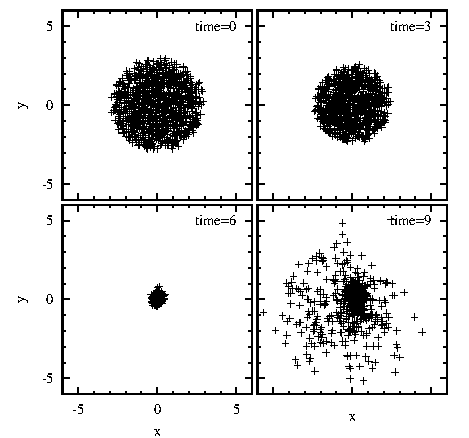
\includegraphics[width=0.75\linewidth]{fig/nbody.pdf}
\end{center}
\caption{}
\label{fig:nbody}
\end{figure}

\describeForEach{% C++用
粒子数を10000個にして計算を行いたい場合には以下のように実行すればよい(MPIを使用しない場合)。
\begin{screen}
\texttt{\$ ./nbody.out -N 10000}
\end{screen}
}{% Fortran用
粒子数を10000個にして計算を行いたい場合には、ファイル\texttt{f\_main.F90}の中のサブルーチン\texttt{f\_main()}のパラメータ変数\texttt{ntot}を10000に設定し、再度、コンパイルした上で実行すればよい。
}{%C言語用
粒子数を10000個にして計算を行いたい場合には、ファイル\texttt{c\_main.c}の中の関数\texttt{c\_main()}の変数\texttt{ntot}を10000に設定し、再度、コンパイルした上で実行すればよい。
}


%%%%%%%%%%%%%%%%
\subsubsubsection{x86版Phantom-GRAPEを使う場合}
\label{s3sec:phantom_grape_x86}
Phantom-GRAPEはSIMD命令を効率的に活用することで重力相互作用の計算を高速に実行するライブラリである(詳細はTanikawa et al.[2012, New Astronomy, 17, 82] とTanikawa et al.[2012, New Astronomy, 19, 74]を参照のこと)。

まず、使用環境を確認する。SIMD命令セットAVXをサポートするIntel CPUまたはAMD CPUを搭載したコンピュータを使用しているならば、x86版Phantom-GRAPEを使用可能である。

次にディレクトリ\texttt{\$(FDPS)/src/phantom\_grape\_x86/G5/newton/libpg5}に移動して、ファイル\texttt{Makefile}を編集し、コマンド\texttt{make}を実行してPhantom-GRAPEのライブラリ\texttt{libpg5.a}を作る。

最後に、ディレクトリ\dirNameNbodySample に戻り、ファイル\texttt{Makefile}内の\texttt{\\''\#use\_phantom\_grape\_x86 = yes''}の\texttt{''\#''}を消す。\texttt{make}を実行してコンパイルする(OpenMP, MPIの使用・不使用どちらにも対応)と、x86版Phantom-GRAPEを使用したコードができている。上と同様の方法で実行・結果の確認を行うとさきほどと同様の結果が得られる。

Intel Core i5-3210M CPU @ 2.50GHz の2コアで性能テスト(OpenMP使用、MPI不使用)をした結果、粒子数8192の場合に、Phantom-GRAPEを使うと、使わない場合に比べて、最大で5倍弱ほど高速なコードとなる。
\describeForCpp{%C++用
以下が最適化された実行例。
\begin{screen}
\texttt{\$ ./nbody.out -N 8192 -n 256}
\end{screen}
ここで、オプション「-n 数値」で相互作用リストを共有する粒子数の上限を指定している。
}

%%%%%%%%%%%%%%%%
\subsubsubsection{PIKGを使う場合}
\label{s3sec:pikg_x86}
PIKGはDSL(ドメイン固有言語)記述から様々なアーキテクチャ向けに最適化された粒子間相互作用カーネルを生成するカーネルジェネレータである.

ディレクトリ\dirNameNbodySample のファイル\texttt{Makefile}内の\texttt{\\''\#use\_pikg\_x86 = yes''}の\texttt{''\#''}を消す。
\describeForEach{% C++用
この状態で\texttt{make}を実行してコンパイルする(OpenMP, MPIの使用・不使用どちらにも対応)と、PIKGから生成されたカーネルを使用した実行ファイル\texttt{nbody.out}ができている。
}{% Fortran用
この状態で\texttt{make}を実行してコンパイルする(OpenMP, MPIの使用・不使用どちらにも対応)と、PIKGから生成されたカーネルを使用した実行ファイル\texttt{nbody.out}ができている。
}{% C言語用
この状態で\texttt{make}を実行してコンパイルする(OpenMP, MPIの使用・不使用どちらにも対応)と、PIKGから生成されたカーネルを使用した実行ファイル\texttt{nbody.out}ができている。
}
上と同様の方法で実行・結果の確認を行うとさきほどと同様の結果が得られる。

デフォルトでは,通常の \progLangName コードと同等の\texttt{reference}モードの相互作用カーネルが生成される.\texttt{Makefile}内の\texttt{\#COVERSION\_TYPE}とその直後にある
\describeForEach{\texttt{\#CFLAGS}}{\texttt{\#CXXFLAGS}}{\texttt{\#CXXFLAGS}}
の行のコメントアウトを外すと,別のアーキテクチャ(AVX2やAVX-512)向けにコードを生成できる.
AVX2モードを使う場合は,利用するCPUがAVX2及びFMAに対応していなくてはならない.さらにAVX-512モードを使う場合には利用するCPUがAVX-512FおよびAVX-512DQに対応していなくてはならない.

\ifCpp % C++用 (subsubsubsectionが1つ含まれている)
%%%%%%%%%%%%%%%%
\subsubsubsection{NVIDIAのGPUを使う場合}
\label{sec:use_nvidia_gpu}
サンプルにはCUDAによって書かれたNVIDIAのGPU用のカーネルも付属している。ディレクトリ\dirNameNbodySample の中のファイル\texttt{Makefile}内の\texttt{\\''\#use\_cuda\_gpu = yes''}の\texttt{''\#''}を消し、更に自分の環境に応じて、\texttt{CUDA\_HOME}の場所を設定する。\texttt{make}を実行してコンパイルする(OpenMP, MPIの使用・不使用どちらにも対応)と、GPUを使用したコードができている。上と同様の方法で実行・結果の確認を行うとさきほどと同様の結果が得られる。
\endifCpp

%%%%%%%%%%%%%%%%%%%%%%%%%%%%%%%
\subsubsection{SPHシミュレーションコード}
\label{subsubsec:usage_of_sample_codes:sph}
本サンプルコードには標準SPH法がFDPSを使って実装されている。簡単のため、smoothing lengthは一定値を取ると仮定している。コードでは、3次元の衝撃波管問題の初期条件を生成し、衝撃波管問題を実際に計算する。
%%%%%%%%%%%%%%%%
\subsubsubsection{概要}
以下の手順で本コードを使用できる。
\begin{itemize}
\item ディレクトリ\dirNameSPHSample に移動
\item カレントディレクトリにある\texttt{Makefile}を編集(後述)
\item コマンドライン上で\texttt{make}を実行
\item \texttt{sph.out}ファイルの実行(後述)
\item 結果の解析(後述)
\end{itemize}
%%%%%%%%%%%%%%%%
\subsubsubsection{ディレクトリ移動}
ディレクトリ\dirNameSPHSample に移動する。
%%%%%%%%%%%%%%%%
\subsubsubsection{Makefileの編集}
\describeForEach{% C++用
\texttt{Makefile}の編集の仕方は$N$体計算の場合と同一なので、 第\ref{s3sec:how_to_edit_Makefile_in_nbody}節を参照されたい。
}{% Fortran用
SPHサンプルコードにも、$N$体計算のサンプルコードの場合と同様、GCCとIntelコンパイラ用に2種類のMakefileが用意されている。編集の仕方は、$N$体計算の場合と同一なので、 第\ref{s3sec:how_to_edit_Makefile_in_nbody}節を参照されたい。
}{% C言語用
\texttt{Makefile}の編集の仕方は$N$体計算の場合と同一なので、 第\ref{s3sec:how_to_edit_Makefile_in_nbody}節を参照されたい。
}

%%%%%%%%%%%%%%%%
\subsubsubsection{\texttt{make}の実行}
\texttt{make}コマンドを実行する。
\describeForIF{% Fortran,C言語版
$N$体計算のときと同様、このとき、まずFDPSの\progLangName インターフェースプログラムが生成され、その後、インターフェースプログラムとサンプルコードが一緒にコンパイルされる。
}

%%%%%%%%%%%%%%%%
\subsubsubsection{実行}
実行方法は以下の通りである。
\begin{itemize}
\item MPIを使用しない場合、コマンドライン上で以下のコマンドを実行する
\begin{screen}
\begin{verbatim}
$ ./sph.out
\end{verbatim}
\end{screen}
  
\item MPIを使用する場合、コマンドライン上で以下のコマンドを実行する
\begin{screen}
\begin{verbatim}
$ MPIRUN -np NPROC ./sph.out
\end{verbatim}
\end{screen}
ここで、\texttt{MPIRUN}には\texttt{mpirun}や\texttt{mpiexec}などが、\texttt{NPROC}には使用するMPIプロセスの数が入る。
\end{itemize}

正しく終了すると以下のようなログを出力する。
\begin{screen}
\begin{verbatim}
******** FDPS has successfully finished. ********
\end{verbatim}
\end{screen}

%%%%%%%%%%%%%%%%
\subsubsubsection{結果の解析}
実行するとディレクトリ\texttt{result}にファイルが出力されている。
\describeForEach{% C++用
ファイル名は"00xx.txt"(xには数字が入る)となっている。ファイル名は時刻を表す。
}{% Fortran用
ファイル名は"snap0000x-proc0000y.dat" となっている。ここで、x,yは整数で、それぞれ、時刻とMPIプロセス番号を表す。MPI実行でない場合には、常にy=0である。
}{% C言語用
ファイル名は"snap0000x-proc0000y.dat" となっている。ここで、x,yは整数で、それぞれ、時刻とMPIプロセス番号を表す。MPI実行でない場合には、常にy=0である。
}
出力ファイルフォーマットは1列目から順に粒子のID、粒子の質量、位置のx, y, z座標、粒子のx, y, z軸方向の速度、密度、内部エネルギー、圧力である。

コマンドライン上で以下のコマンドを実行すれば、横軸に粒子のx座標、縦軸に粒子の密度をプロットできる(時刻は40)。
\ifCpp %C++用
\begin{screen}
\begin{verbatim}
$ gnuplot
$ plot "result/0040.txt" using 3:9
\end{verbatim}
\end{screen}
\endifCpp
\ifFtn %Fortran用
\begin{screen}
\begin{verbatim}
$ cd result
$ cat snap00040-proc* > snap00040.dat
$ gnuplot
> plot "snap00040.dat" using 3:9
\end{verbatim}
\end{screen}
\endifFtn
\ifC % C言語用
\begin{screen}
\begin{verbatim}
$ cd result
$ cat snap00040-proc* > snap00040.dat
$ gnuplot
> plot "snap00040.dat" using 3:9
\end{verbatim}
\end{screen}
\endifC
正しい答が得られれば、図\ref{fig:sph}のような図を描ける。

\begin{figure}[h]
\centering
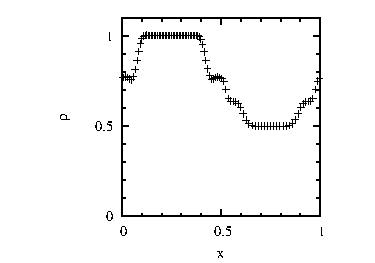
\includegraphics[width=0.5\linewidth]{fig/sph.pdf}
\caption{衝撃波管問題の時刻$t=40$における密度分布}
\label{fig:sph}
\end{figure}

\clearpage

%%%%%%%%%%%%%%%%%%%%%%%%%%%%%%%%%%%%%%%%%%%%%%%%%%%%%
\section{サンプルコードの解説}
\label{sec:how_to_use}
%================================
%   この節の概要/内容について
%================================
本節では、前節(第\ref{sec:getting_started}節)で動かしたサンプルコードについての解説を行う。特に、ユーザが定義しなければならない\structure (以後、\textbf{ユーザ定義型}と呼ぶ)やFDPSの各種APIの使い方について詳しく述べる。\ul{説明の重複を避けるため、いくつかの事項に関しては、その詳細な説明が{$N$}体シミュレーションコードの節でのみ行われている}。そのため、SPHシミュレーションだけに興味があるユーザも、$N$体シミュレーションコードの節に目を通して頂きたい。

%======================
%   N体コード
%======================
\subsection{$N$体シミュレーションコード}
\label{subsec:how_to_use:nbody}

\subsubsection{ソースファイルの場所と構成}
ソースファイルは\dirNameNbodySample 以下にある。
\describeForEach{%C++用
サンプルコードは、次節で説明するユーザ定義型が記述されたソースコード \path{user-defined.hpp} と、$N$体シミュレーションのメインループ等が記述されたソースコード\path{main.cpp}から構成される。この他に、GCC用の\path{Makefile}がある。

}{%Fortran用
サンプルコードは、次節で説明するユーザ定義型が記述されたソースコード \path{user_defined.F90} と、$N$体シミュレーションのメインループ等が記述されたソースコード\path{f_main.F90}から構成される。この他に、GCCとIntelコンパイラ用のMakefileである\path{Makefile}と\path{Makefile.intel}がある。
}{%C用
サンプルコードは、次節で説明するユーザ定義型が記述されたソースコード \path{user_defined.h} と、相互作用関数が定義された\path{user_defined.c}、$N$体シミュレーションのメインループ等が記述されたソースコード\path{c_main.c}から構成される。この他に、GCC用の\path{Makefile}がある。
}

\subsubsection{ユーザー定義型・ユーザ定義関数}
本節では、FDPSの機能を用いて$N$体計算を行う際、ユーザーが記述しなければならない\structure と \procedure について記述する。

%-----------------------
%   FullParticle type
%-----------------------
\subsubsubsection{FullParticle型}
ユーザーはユーザ定義型の1つFullParticle型を記述しなければならない。FullParticle型には、シミュレーションを行うにあたって、$N$体粒子が持っているべき全ての物理量が含まれている。Listing~\ref{nbody_FP}に本サンプルコードのFullParticle型の実装例を示す(\describeForEach{user-defined.hpp}{\texttt{user\_defined.F90}}{\texttt{user\_defined.h}}を参照)。

\ifCpp%C++用
\lstinputlisting[linerange={17-65},caption=FullParticle型,label=nbody_FP]{../../../../sample/c++/nbody/user-defined.hpp}
\endifCpp
\ifFtn%Fortran用
\lstinputlisting[linerange={14-24},caption=FullParticle型,label=nbody_FP]{../../../../sample/fortran/nbody/user_defined.F90}
\endifFtn
\ifC%C言語
\lstinputlisting[linerange={7-18},caption=FullParticle型,label=nbody_FP]{../../../../sample/c/nbody/user_defined.h}
\endifC

\describeForCpp{%C++用
\ul{本サンプルコードでは、FullParticle型がEssentialParticleI型、EssentialParticleJ型、そして、Force型を兼ねている}。また、FullParticle型には、データのコピーするのに必要なメンバ関数\texttt{copyFromFP}と\texttt{copyFromForce}を持たせている。その他、粒子質量を返す関数である\texttt{getCharge}、粒子座標を返す関数である\texttt{getPos}が必要になる。また、積算対象のメンバ変数である加速度とポテンシャルを0クリアするための関数\texttt{clear}が必要になる。本サンプルコードでは、FDPSに備わっているファイル入出力関数を使用するため、それに必要な関数である\texttt{writeAscii()}と\texttt{readAscii()}を書いてある。
}

\describeForIF{% Fortran,C用
FDPS \progLangName インターフェースを使ってユーザコードを開発する場合、ユーザは\structure がどのユーザ定義型(FullParticle型, EssentialParticleI型, EssentialParticleJ型, Force型)に対応するかをFDPSに教えなければならない。本インターフェースにおいて、この指示は、\structure に決まった書式のコメント文を加えることによって行う(以後、この種のコメント文を\textbf{FDPS指示文}と呼ぶ)。本サンプルコードでは、FullParticle型がEssentialParticleI型、EssentialParticleJ型、そして、Force型を兼ねている。そのため、\structure がすべてのユーザ定義型に対応すること指示する以下のコメント文を記述している:
}
\ifFtn %Fortran用
\begin{screen}
\begin{spverbatim}
type, public, bind(c) :: full_particle !$fdps FP,EPI,EPJ,Force
\end{spverbatim}
\end{screen}
\endifFtn
\ifC %C言語用
\begin{screen}
\begin{spverbatim}
typedef struct full_particle { //$fdps FP,EPI,EPJ,Force
\end{spverbatim}
\end{screen}
\endifC

\describeForIF{%Fortran,C用
また、FDPSはFullParticle型のどのメンバ変数が質量や位置等の\textbf{必須物理量}(どの粒子計算でも必ず必要となる物理量、或いは、特定の粒子計算において必要とされる物理量と定義する)に対応するのかを知っていなければならない。この指示も決まった書式のコメント文をメンバ変数に対して記述することで行う。今回の例では、メンバ変数\texttt{mass}, \texttt{pos}, \texttt{vel}が、それぞれ、質量、位置、速度に対応することをFDPSに指示するため、以下の指示文が記述されている:
}
\ifFtn %Fortran用
\begin{screen}
\begin{spverbatim}
real(kind=c_double) :: mass !$fdps charge
type(fdps_f64vec) :: pos !$fdps position
type(fdps_f64vec) :: vel !$fdps velocity
\end{spverbatim}  
\end{screen}
\endifFtn
\ifC %C言語用
\begin{screen}
\begin{spverbatim}
double mass; //$fdps charge
fdps_f64vec pos; //$fdps position
fdps_f64vec vel; //$fdps velocity
\end{spverbatim}  
\end{screen}
\endifC
\describeForIF{%Fortran,C用
ただし、メンバ変数が速度であることを指示する\describeForEach{}{\texttt{!\$fdps velocity}}{\texttt{//\$fdps velocity}}は予約語であり、指示は任意である(現時点でFDPSの振舞に一切影響しない)。

FullParticle型はEssentialParticleI型、EssentialParticleJ型、Force型との間でデータの移動(データコピー)を行う。ユーザはこのコピーの仕方を指示するFDPS指示文も記述しなければならない。本サンプルコードでは、以下のように記述している:
}
\ifFtn %Fortran用
\begin{screen}
\begin{spverbatim}
!$fdps copyFromForce full_particle (pot,pot) (acc,acc)
!$fdps copyFromFP full_particle (id,id) (mass,mass) (pos,pos)
\end{spverbatim}  
\end{screen}
\endifFtn
\ifC %C言語
\begin{screen}
\begin{spverbatim}
//$fdps copyFromForce full_particle (pot,pot) (acc,acc)
//$fdps copyFromFP full_particle (id,id) (mass,mass) (pos,pos)
\end{spverbatim}  
\end{screen}
\endifC
\describeForIF{%Fortran,C用
ここで、キーワード\texttt{copyFromForce}を含む指示文は、Force型のどのメンバ変数をFullParticle型のどのメンバ変数にコピーするのかを指示するもので、FullParticle型に\ulBold{常に}記述しなければならない指示文である。一方、キーワード\texttt{copyFromFP}はFullParticle型からEssentialParticleI型およびEssentialParticleJ型へのデータコピーの仕方を指示するもので、EssentialParticleI型とEssentialParticleJ型には\ulBold{必ず}記述しなければならない指示文である。今、FullParticle型はこれら2つを兼ねているため、ここに記述している。

今、FullParticle型はForce型を兼ねている。Force型にも必ず記述しなければならない指示文がある。それは、相互作用計算において、積算対象のメンバ変数をどのように0クリアするかを指示する指示文である。本サンプルコードでは、積算対象である加速度とポテンシャルのみを0クリアすることを指示するため、次の指示文を記述している:
}
\ifFtn %Fortran用
\begin{screen}
\begin{spverbatim}
!$fdps clear id=keep, mass=keep, pos=keep, vel=keep
\end{spverbatim}
\end{screen}
\endifFtn
\ifC%C言語用
\begin{screen}
\begin{spverbatim}
//$fdps clear id=keep, mass=keep, pos=keep, vel=keep
\end{spverbatim}
\end{screen}
\endifC
\describeForIF{%Fortran,C用
ここで、キーワード\texttt{clear}の右に記述された構文 \texttt{\textit{mbr}=keep} は、メンバ変数\textit{\texttt{mbr}}の値を変更しないことを指示する構文である。

FDPS指示文の書式の詳細については、仕様書\path{doc_specs_ftn_ja.pdf}をご覧頂きたい。
}

%-----------------------
%   calcForceEpEp
%-----------------------
\subsubsubsection{相互作用関数 calcForceEpEp}
ユーザーは粒子間相互作用の仕方を記述した相互作用関数 calcForceEpEpを記述しなければならない。\procedure calcForceEpEpには、粒子-粒子相互作用計算の具体的な内容を書く必要がある。Listing~\ref{nbody_calcForceEpEp}に、本サンプルコードでの実装を示す(\describeForEach{\texttt{user-defined.hpp}}{\texttt{user\_defined.F90}}{\texttt{user\_defined.c}}を参照)。

\ifCpp%C++用
\lstinputlisting[linerange={122-146},caption=関数 calcForceEpEp,label=nbody_calcForceEpEp]{../../../../sample/c++/nbody/user-defined.hpp}
\endifCpp
\ifFtn%Fortran用
\lstinputlisting[linerange={144-191},caption=関数 calcForceEpEp,label=nbody_calcForceEpEp]{../../../../sample/fortran/nbody/user_defined.F90}
\endifFtn
\ifC%C言語用
\lstinputlisting[linerange={3-38},caption=関数 calcForceEpEp,label=nbody_calcForceEpEp]{../../../../sample/c/nbody/user_defined.c}
\endifC

\ifCpp%C++用
ここに示したのは、Phantom-GRAPEライブラリを使用せずにCPUで実行する場合の実装である。

本サンプルコードではテンプレート関数\footnote{テンプレート関数とはC++言語のテンプレート機能を関数に適用することで汎用的な関数としたものである。通常の関数では、関数の型および関数の引数の型をその場ですべて指定して記述/定義するが、テンプレート関数では、\texttt{templete <...>}内に指定された一般的なデータ型・クラスを関数定義に使用することができる(``一般的なクラス"の情報は、関数呼び出しの際にテンプレート引数として渡す。このため、コンパイル時にテンプレート関数のすべての型は問題なく決定される)。これによって、一般的な関数を定義することが可能となる。}を用いて実装している。また、テンプレート関数の引数は、EssentialParticleIの配列、EssentialParticleIの個数、EssentialParticleJの配列、EssentialParticleJの個数、Force型の配列である。
\endifCpp
\ifIF%Fortran,C用
本サンプルコードでは、\procedure \texttt{calc\_gravity\_ep\_ep}として実装されている。\procedure の仮引数は、EssentialParticleIの配列、EssentialParticleIの個数、EssentialParticleJの配列、EssentialParticleJの個数、Force型の配列である。本サンプルコードでは、FullParticle型がすべてのユーザ定義型を兼ねているため、引数のデータ型はすべて\texttt{full\_particle}型となっていることに注意して頂きたい。
\endifIF

%-----------------------
%   calcForceEpSp
%-----------------------
\describeForIF{%Fortran,C用
\subsubsubsection{相互作用関数 calcForceEpSp}
ユーザーは粒子-超粒子間相互作用の仕方を記述した相互作用関数 calcForceEpSpを記述しなければならない。calcForceEpSpには、粒子-超粒子相互作用計算の具体的な内容を書く必要があり、\procedure として実装しなければならない。Listing~\ref{nbody_calcForceEpSp}に、本サンプルコードでの実装を示す(\describeForEach{}{\texttt{user\_defined.F90}}{\texttt{user\_defined.c}}を参照)。
}
\ifFtn%Fortran用
\lstinputlisting[linerange={194-231},caption=関数 calcForceEpSp,label=nbody_calcForceEpSp]{../../../../sample/fortran/nbody/user_defined.F90}
\endifFtn
\ifC%C言語用
\lstinputlisting[linerange={40-75},caption=関数 calcForceEpSp,label=nbody_calcForceEpSp]{../../../../sample/c/nbody/user_defined.c}
\endifC
\describeForIF{%Fortran,C用
本サンプルコードでは、\procedure \texttt{calc\_gravity\_ep\_sp}として実装されている。\procedure の仮引数は、EssentialParticleIの配列、EssentialParticleIの個数、超粒子の配列、超粒子の個数、Force型の配列である。本サンプルコードでは、FullParticle型がすべてのユーザ定義型を兼ねているため、引数のForce型は\texttt{full\_particle}型となっていることに注意して頂きたい。ここで指定する超粒子型はこの相互作用計算を実施するのに使用するツリーオブジェクトの種別と適合していなければならない。
}

\subsubsection{プログラム本体}
\label{subsubsec:nbody_sample_main_part}
\describeForCpp{%C++用
本節では、FDPSを用いて$N$体計算を行うにあたり、メイン関数に書かれるべき関数に関して解説する。メイン関数はサンプルコード\texttt{nbody.cpp}内に記述されている。
}
\describeForIF{%Fortran,C用
本節では、FDPS \progLangName インターフェースを用いて$N$体計算を行うにあたり、``\mainFunc" \mainFuncName に書かれるべき\procedure や\function に関して解説する。ここで、\mainFunc とはっきり書かないのは、次の理由による: FDPS \progLangName インターフェースを使用する場合、ユーザコードは必ず\usaw{\procedure} \mainFuncName の下に記述されなければならず、ユーザコードは正しい意味での\mainFunc を持たない(\mainFunc はインターフェースプログラムのC++ソースコード内にある)。しかし、実質的には\procedure \mainFuncName が\mainFunc の役割を果たす。そのため、敢えて``\mainFunc"という言葉を使った。\mainFunc という言葉は、それがユーザコードの入り口であることを示すのに適しているので、以後、\mainFuncName を\mainFunc と呼ぶことにする。本サンプルコードの\mainFunc は\fileNameOfMainFunc に記述されている。
}

\ifCpp%C++用
\subsubsubsection{ヘッダーファイルのインクルード}
FDPSの標準機能を利用できるようにするため、\texttt{particle\_simulator.hpp}をインクルードする。
\begin{lstlisting}[caption=ヘッダーファイル\texttt{particle\_simulator.hpp}のインクルード]
#include <particle_simulator.hpp>
\end{lstlisting}
\endifCpp
\ifFtn%Fortran用
\subsubsubsection{\texttt{fdps\_controller}型オブジェクトの生成}
FDPS Fortran インターフェースにおいて、FDPSのAPIはすべてFortran 2003のクラス\texttt{FDPS\_controller}のメンバ関数として提供される。このクラスは、インターフェースプログラムの1つである\texttt{FDPS\_module.F90}の中の、モジュール\texttt{fdps\_module}内で定義されている。したがって、ユーザはFDPSのAPIを使用するために、\texttt{FDPS\_controller}型オブジェクトを生成しなければならない。本サンプルコードでは、\texttt{FDPS\_controller}型オブジェクト\texttt{fdps\_ctrl}をメインルーチンで生成している:
\begin{lstlisting}[caption=\texttt{fdps\_controller}型オブジェクトの生成]
subroutine f_main()
   use fdps_module
   implicit none
   !* Local variables
   type(fdps_controller) :: fdps_ctrl
    
   ! Do something
   
end subroutine f_main    
\end{lstlisting}
ここに示したコードは実際にサンプルコードから必要な部分だけを取り出したものであることに注意して頂きたい。

上記の理由から、以下の説明において、FDPSのAPIはこのオブジェクトのメンバ関数として呼び出されていることに注意されたい。
\endifFtn
\ifC %C言語用
\subsubsubsection{ヘッダーファイルのインクルード}
FDPSの標準機能を利用できるようにするため、\texttt{FDPS\_c\_if.h}をインクルードする。
\begin{lstlisting}[caption=ヘッダーファイル\texttt{FDPS\_c\_if.h}のインクルード]
#include "FDPS_c_if.h"
\end{lstlisting}
\endifC

\subsubsubsection{開始、終了}
まずは、FDPSの初期化/開始を行う必要がある。次のように、\mainFunc に記述する。
\ifCpp%C++用
\begin{lstlisting}[caption=FDPSの開始]
PS::Initialize(argc, argv);
\end{lstlisting}
\endifCpp
\ifFtn%Fortran用
\begin{lstlisting}[caption=FDPSの開始]
call fdps_ctrl%ps_initialize()
\end{lstlisting}
\endifFtn
\ifC%C言語用
\begin{lstlisting}[caption=FDPSの開始]
fdps_initialize();
\end{lstlisting}
\endifC


FDPSは、開始したら明示的に終了させる必要がある。今回は、プログラムの終了と同時にFDPSも終了させるため、\mainFunc の最後に次のように記述する。
\ifCpp%C++用
\begin{lstlisting}[caption=FDPSの終了]
PS::Finalize();
\end{lstlisting}
\endifCpp
\ifFtn%Fortran用
\begin{lstlisting}[caption=FDPSの終了]
call fdps_ctrl%ps_finalize()
\end{lstlisting}
\endifFtn
\ifC%C言語用
\begin{lstlisting}[caption=FDPSの終了]
fdps_finalize();
\end{lstlisting}
\endifC

\subsubsubsection{オブジェクトの生成・初期化}
FDPSの初期化に成功した場合、ユーザーはコード中で用いるオブジェクトを作成する必要がある。本節では、オブジェクトの生成/初期化の仕方について解説する。

\subsubsubsubsection{オブジェクトの生成}
\ifCpp%C++用
今回の計算では、粒子群クラス、領域クラスに加え、重力計算用の相互作用ツリーを一本生成する必要がある。以下にそのコードを記す。これらはサンプルコード\texttt{nbody.cpp}の\texttt{main}関数内に記述されている。
\begin{lstlisting}[caption=オブジェクトの生成]
PS::DomainInfo dinfo;
PS::ParticleSystem<FPGrav> system_grav;
PS::TreeForForceLong<FPGrav, FPGrav, FPGrav>::Monopole tree_grav;
\end{lstlisting}
\endifCpp
\describeForIF{%Fortran,C用
今回の計算では、粒子群オブジェクト、領域情報オブジェクトに加え、重力計算用のツリーオブジェクトを1個生成する必要がある。\progLangName インターフェースでは、これらオブジェクトはすべて整数変数に格納された識別番号を使って操作する。したがって、まず識別番号を格納する整数変数を用意したあとに、オブジェクトを生成するAPIを呼び出す必要がある。以下にそのコードを記す。これらはサンプルコード\fileNameOfMainFunc の\mainFunc 内に記述されている。
}
\ifFtn%Fortran用
\begin{lstlisting}[caption=オブジェクトの生成]
subroutine f_main()
   use fdps_module
   use user_defined_types
   implicit none
   !* Local variables
   integer :: psys_num,dinfo_num,tree_num
   
   !* Create FDPS objects
   call fdps_ctrl%create_dinfo(dinfo_num)
   call fdps_ctrl%create_psys(psys_num,'full_particle')
   call fdps_ctrl%create_tree(tree_num, &
                              "Long,full_particle,full_particle,full_particle,Monopole")

end subroutine f_main
\end{lstlisting}
\endifFtn
\ifC%C言語用
\begin{lstlisting}[caption=オブジェクトの生成]
void c_main() {
   
    // Create and initialize dinfo object
    int dinfo_num;
    fdps_create_dinfo(&dinfo_num);
    // Create and initialize psys object
    int psys_num;
    fdps_create_psys(&psys_num,"full_particle");
    // Create and initialize tree object
    int tree_num;
    fdps_create_tree(&tree_num,
                     "Long,full_particle,full_particle,full_particle,Monopole");

}
\end{lstlisting}
\endifC
\describeForIF{%Fortran,C用
ここでも、実際のサンプルコードから該当部分だけを抜き出していることに注意して頂きたい。

上に示すように、粒子群オブジェクトを生成する際にはFullParticle型に対応する\structure 名を文字列としてAPIの引数に渡す必要がある。同様に、ツリーオブジェクト生成の際には、ツリーの種別を示す文字列をAPIの引数に渡す必要がある。両APIにおいて、\textbf{\ul{{\structure} 名は小文字で入力されなければならない}}。
}

\subsubsubsubsection{領域情報オブジェクトの初期化}
ユーザーはオブジェクトを作成したら、そのオブジェクトの初期化を行う必要がある。本サンプルコードでは周期境界等は用いていないため、領域情報オブジェクトの初期化はAPI \initDinfo を実行するだけでよい:
\ifCpp%C++用
\begin{lstlisting}[caption=領域クラスの初期化]
const PS::F32 coef_ema = 0.3;
dinfo.initialize(coef_ema);
\end{lstlisting}
\endifCpp
\ifFtn%Fortran用
\begin{lstlisting}[caption=領域オブジェクトの初期化]
call fdps_ctrl%init_dinfo(dinfo_num,coef_ema)
\end{lstlisting}
\endifFtn
\ifC%C言語用
\begin{lstlisting}[caption=領域オブジェクトの初期化]
fdps_init_dinfo(dinfo_num,coef_ema);
\end{lstlisting}
\endifC
ここで、API \initDinfo の第\describeForEach{1}{2}{2}引数は領域分割に使用される指数移動平均の平滑化係数を表す。この係数の意味については仕様書に詳しい解説があるので、そちらを参照されたい。

\subsubsubsubsection{粒子群オブジェクトの初期化}
次に、粒子群オブジェクトの初期化を行う必要がある。粒子群オブジェクトの初期化は、API \initPsys で行う:
\ifCpp%C++用
\begin{lstlisting}[caption=粒子群クラスの初期化]
system_grav.initialize();
\end{lstlisting}
\endifCpp
\ifFtn%Fortran用
\begin{lstlisting}[caption=粒子群オブジェクトの初期化]
call fdps_ctrl%init_psys(psys_num)
\end{lstlisting}
\endifFtn
\ifC%C言語
\begin{lstlisting}[caption=粒子群オブジェクトの初期化]
fdps_init_psys(psys_num);
\end{lstlisting}
\endifC

\subsubsubsubsection{ツリーオブジェクトの初期化}
次に、ツリーオブジェクトの初期化を行う必要がある。ツリーオブジェクトの初期化はAPI \initTree で行う。このAPIには、引数として大雑把な粒子数を渡す必要がある。今回は、全体の粒子数(\texttt{ntot})をセットしておく事にする:
\ifCpp%C++用
\begin{lstlisting}[caption=相互作用ツリークラスの初期化]
tree_grav.initialize(n_tot, theta, n_leaf_limit, n_group_limit);
\end{lstlisting}
\endifCpp
\ifFtn%Fortran用
\begin{lstlisting}[caption=ツリーオブジェクトの初期化]
call fdps_ctrl%init_tree(tree_num,ntot,theta, &
                         n_leaf_limit,n_group_limit)
\end{lstlisting}
\endifFtn
\ifC%C言語
\begin{lstlisting}[caption=ツリーオブジェクトの初期化]
fdps_init_tree(tree_num,ntot,theta,
               n_leaf_limit,n_group_limit);
\end{lstlisting}
\endifC

\describeForEach{%C++用
このAPIには3つの省略可能引数が存在し、サンプルコードではこれらを省略せずに指定している:
}{%Fortran用
このAPIには3つの省略可能引数が存在し、サンプルコードではこれらを省略せずに指定している:
}{%C言語
このAPIの第3引数以降の引数の意味は次の通りである:
}
\begin{itemize}[leftmargin=*,itemsep=-1ex,topsep=0.2ex]
\item \texttt{theta} --- ツリー法で力の計算をする場合の見込み角についての基準
\item \texttt{n\_leaf\_limit} --- ツリーを切るのをやめる粒子数の上限
\item \texttt{n\_group\_limit} --- 相互作用リストを共有する粒子数の上限
\end{itemize}

\describeForIF{%Fortran,C用
\subsubsubsection{粒子データの初期化}
\label{s3sec:nbody_initialize_ptcl_data}
初期条件の設定を行うためには、粒子群オブジェクトに粒子データを入力する必要がある。(既にAPI \initPsys で初期化済みの)粒子群オブジェクトに、FullParticle型粒子のデータを格納するには、粒子群オブジェクトのAPI \setNptclLoc と \getPsysPtr を用いて、次のように行う:
}
\ifFtn%Fortran用
\begin{lstlisting}[caption=粒子データの初期化]
subroutine foo(fdps_ctrl,psys_num)
   use fdps_vector
   use fdps_module
   use user_defined_types
   implicit none
   type(fdps_controller), intent(IN) :: fdps_ctrl
   integer, intent(IN) :: psys_num
   !* Local variables
   integer :: i,nptcl_loc
   type(full_particle), dimension(:), pointer :: ptcl

   !* Set # of local particles
   call fdps_ctrl%set_nptcl_loc(psys_num,nptcl_loc)

   !* Get the pointer to full particle data
   call fdps_ctrl%get_psys_fptr(psys_num,ptcl)
   
   !* Initialize particle data
   do i=1,nptcl_loc
      ptcl(i)%pos = ! Do something
   end do
   
   !* Release the pointer
   nullify(ptcl)

end subroutine foo
\end{lstlisting}
\endifFtn
\ifC%C言語用
\begin{lstlisting}[caption=粒子データの初期化]
void foo(psys_num) {
   // Set # of local particles
   nptcl_loc = 1024; 
   fdps_set_nptcl_loc(psys_num,nptcl_loc);

   // Get the pointer to full particle data
   Full_particle *ptcl = (Full_particle *)  fdps_get_psys_cptr(psys_num);
   
   // Initialize particle data
   int i;
   for (i = 0; i < nptcl_loc; i++) {
      ptcl[i].pos.x = /* Do something */ ;
   }
   
}
\end{lstlisting}
\endifC
\describeForIF{%Fortran,C用
まず、粒子群オブジェクトに粒子データを保存するのに必要なメモリを確保しなければならない。これを行うには API \setNptclLoc を実行すればよい。このAPIは指定された粒子群オブジェクトのローカル粒子数(自プロセスが管理する粒子数)の値を設定し、かつ、その粒子数を格納するのに必要なメモリを確保する。粒子データを初期化するためには、確保されたメモリのアドレスを取得しなければならない。これにはAPI \getPsysPtr を使用する。
}
\ifFtn%Fortran用
アドレスはFortranポインタで受け取る必要がある。そのため、上記の例では、ポインタを以下のように用意している:
\begin{screen}
\begin{spverbatim}
type(full_particle), dimension(:), pointer :: ptcl
\end{spverbatim}  
\end{screen}
API \texttt{get\_psys\_fptr}によってポインタを設定した後は、ポインタを粒子配列のように使用することが可能である。上の例では、粒子データの設定が完了した後、ポインタを組込関数\texttt{nullify}によって解放している。
\endifFtn
\ifC%C言語用
アドレスは\texttt{void *}ポインタとして返ってくるため、\texttt{Full\_particle *}型にキャストしていること注意されたい。API \getPsysPtr によってポインタを設定した後は、ポインタを粒子配列のように使用することが可能である。
\endifC

\subsubsubsection{ループ}
本節では、時間積分ループの中で行わなければならないことについて、解説する。

\subsubsubsubsection{領域分割の実行}
まずは、粒子分布に基いて、領域分割を実行する。本サンプルコードでは、これを領域情報オブジェクトのAPI \decomposeDomainAll を用いて行っている:
\ifCpp%C++用
\begin{lstlisting}[caption=領域分割の実行]
if(n_loop % 4 == 0){
   dinfo.decomposeDomainAll(system_grav);
}
\end{lstlisting}
\endifCpp
\ifFtn%Fortran用
\begin{lstlisting}[caption=領域分割の実行]
if (mod(num_loop,4) == 0) then
   call fdps_ctrl%decompose_domain_all(dinfo_num,psys_num)
end if
\end{lstlisting}
\endifFtn
\ifC%C言語用
\begin{lstlisting}[caption=領域分割の実行]
if (num_loop % 4 == 0) {
   fdps_decompose_domain_all(dinfo_num,psys_num,-1.0);
}
\end{lstlisting}
\endifC
ここで、計算時間の節約のため、領域分割は4ループ毎に1回だけ行うようにしている。
\describeForC{第3引数は、領域分割する際に、自プロセスからどれだけ粒子をサンプリングするかを表す``重み"を表す変数である。この変数は$>0$である必要があるが、負値が指定された場合、FDPSのデフォルト値が採用される。詳細は仕様書を参照されたい。}

\subsubsubsubsection{粒子交換の実行}
次に、領域情報に基いて、プロセス間の粒子の情報を交換する。これには、粒子群オブジェクトのAPI \exchangeParticle を用いる:
\ifCpp%C++用
\begin{lstlisting}[caption=粒子交換の実行]
system_grav.exchangeParticle(dinfo);
\end{lstlisting}
\endifCpp
\ifFtn%Fortran用
\begin{lstlisting}[caption=粒子交換の実行]
call fdps_ctrl%exchange_particle(psys_num,dinfo_num)
\end{lstlisting}
\endifFtn
\ifC%C言語用
\begin{lstlisting}[caption=粒子交換の実行]
fdps_exchange_particle(psys_num,dinfo_num);
\end{lstlisting}
\endifC


\subsubsubsubsection{相互作用計算の実行}
領域分割・粒子交換が終了したら、相互作用の計算を行う。これには、ツリーオブジェクトのAPI \calcForceAllAndWriteBack を用いる:
\ifCpp%C++用
\begin{lstlisting}[caption=相互作用計算の実行]
tree_grav.calcForceAllAndWriteBack(CalcGravity<FPGrav>,
                                   CalcGravity<PS::SPJMonopole>,
                                   system_grav,
                                   dinfo);
\end{lstlisting}
ここで、メソッドの引数に\texttt{CalcGravity<....>}のような記述があるが、この\texttt{<...>}内に書かれているものがテンプレート引数である。
\endifCpp
\ifFtn%Fortran用
\begin{lstlisting}[caption=相互作用計算の実行]
subroutien f_main()
   use, intrinsic :: iso_c_binding
   use user_defined_types
   implicit none
   !* Local variables
   type(c_funptr) :: pfunc_ep_ep,pfunc_ep_sp
   
   ! Do somehting
   
   pfunc_ep_ep = c_funloc(calc_gravity_ep_ep)
   pfunc_ep_sp = c_funloc(calc_gravity_ep_sp)
   call fdps_ctrl%calc_force_all_and_write_back(tree_num,    &
                                                pfunc_ep_ep, &
                                                pfunc_ep_sp, &
                                                psys_num,    &
                                                dinfo_num)

   ! Do something

end subroutine f_main
\end{lstlisting}
ここで、APIの第2,3引数には関数calcForceEpEp, calcForceEpSpの(C言語アドレス\footnote{C言語方式で記述されたアドレス情報のこと。}としての)関数ポインタを指定する。関数のC言語アドレスは、Fortran 2003で導入された組込関数\texttt{c\_funloc}を使って取得する(この組込み関数はモジュール\texttt{iso\_c\_binding}で提供されるため、\texttt{use}文を使い、このモジュールを利用可能にしている)。C言語アドレスを格納するためには、同じくFortran 2003で導入された派生データ型 \texttt{c\_funptr}の変数が必要である。そのため、本サンプルコードでは、\texttt{c\_funptr}型変数として、\texttt{pfunc\_ep\_ep}と\texttt{pfunc\_ep\_sp}を用意している。ここに、\texttt{calc\_gravity\_ep\_ep}と\texttt{calc\_gravity\_ep\_sp}のC言語アドレスを格納した上で、APIに渡している。
\endifFtn
\ifC%C言語用
\begin{lstlisting}[caption=相互作用計算の実行]
void c_main() {
   
   // Do somehting
   
   fdps_calc_force_all_and_write_back(tree_num,
                                      calc_gravity_ep_ep,
                                      calc_gravity_ep_sp,
                                      psys_num,
                                      dinfo_num,
                                      true,
                                      FDPS_MAKE_LIST);

   // Do something

}
\end{lstlisting}
ここで、APIの第2,3引数には関数calcForceEpEp, calcForceEpSpの関数ポインタを指定する。第6引数には、前回の相互作用計算の結果をクリアするかどうかを\texttt{\_Bool}値で指定する。第7引数は、相互作用リストの再利用を行うかどうかを指示するフラグで、ここでは新規に相互作用リストを作成して相互作用計算を行うモードを選択している。
\endifC


\subsubsubsubsection{時間積分} \label{s4sec:nbody_time_integration}
本サンプルコードでは、時間積分をLeapfrog時間積分法によって行う。時間積分は形式的に、$K(\frac{\Delta t}{2})D(\Delta t)K(\frac{\Delta t}{2})$と表される。ここで、$\Delta t$は時間刻み、$K(\cdot)$は速度を指定された時間だけ時間推進するオペレータ、$D(\cdot)$は位置を指定された時間だけ時間推進するオペレータである。本サンプルコードにおいて、これらのオペレータは、\procedure \texttt{kick}と\procedure \texttt{drift}として実装している。

時間積分ループの最初で、最初の$D(\Delta t)K(\frac{\Delta t}{2})$の計算を行い、粒子の座標と速度の情報を更新している:
\ifCpp%C++用
\begin{lstlisting}[caption=$D(\Delta t)K(\frac{\Delta t}{2})$オペレータの計算]
kick(system_grav, dt * 0.5);
drift(system_grav, dt);
\end{lstlisting}
\endifCpp
\ifFtn%Fortran用
\begin{lstlisting}[caption=$D(\Delta t)K(\frac{\Delta t}{2})$オペレータの計算]
!* Leapfrog: Kick-Drift
call kick(fdps_ctrl,psys_num,0.5d0*dt)
time_sys = time_sys + dt
call drift(fdps_ctrl,psys_num,dt)
\end{lstlisting}
\endifFtn
\ifC%C言語用
\begin{lstlisting}[caption=$D(\Delta t)K(\frac{\Delta t}{2})$オペレータの計算]
// Leapfrog: Kick-Drift
kick(psys_num,0.5*dt);
time_sys +=  dt;
drift(psys_num,dt);
\end{lstlisting}
\endifFtn


時間積分ループの次の部分では、力の計算を行い、その後、最後の$K(\frac{\Delta t}{2})$の計算を行っている:
\ifCpp%C++用
\begin{lstlisting}[caption=$K(\frac{\Delta t}{2})$オペレータの計算]
kick(system_grav, dt * 0.5);
\end{lstlisting}
\endifCpp
\ifFtn%Fortran用
\begin{lstlisting}[caption=$K(\frac{\Delta t}{2})$オペレータの計算]
!* Leapfrog: Kick
call kick(fdps_ctrl,psys_num,0.5d0*dt)
\end{lstlisting}
\endifFtn
\ifC%C言語用
\begin{lstlisting}[caption=$K(\frac{\Delta t}{2})$オペレータの計算]
// Leapfrog: Kick
kick(psys_num,0.5d0*dt);
\end{lstlisting}
\endifC

\describeForIF{%Fortran,C用
\subsubsubsection{粒子データの更新}
上記で説明した\texttt{kick}や\texttt{drift}等の\procedure で、粒子データを更新するためには、粒子群オブジェクトに格納されている粒子データにアクセスする必要がある。これは、第\ref{s3sec:nbody_initialize_ptcl_data}節で説明した方法とほぼ同様に行う:
}
\ifFtn%Fortran用
\begin{lstlisting}[caption=粒子データの更新]
subroutine foo(fdps_ctrl,psys_num)
   use fdps_vector
   use fdps_module
   use user_defined_types
   implicit none
   type(fdps_controller), intent(IN) :: fdps_ctrl
   integer, intent(IN) :: psys_num
   !* Local variables
   integer :: i,nptcl_loc
   type(full_particle), dimension(:), pointer :: ptcl

   !* Get # of local particles
   nptcl_loc = fdps_ctrl%get_nptcl_loc(psys_num)

   !* Get the pointer to full particle data
   call fdps_ctrl%get_psys_fptr(psys_num,ptcl)
   
   !* Initialize or update particle data
   do i=1,nptcl_loc
      ptcl(i)%pos = ! Do something
   end do
   
   !* Release the pointer
   nullify(ptcl)

end subroutine foo
\end{lstlisting}
API \getPsysPtr を使い、粒子群オブジェクトに格納された粒子データのアドレスをポインタとして受け取る。受け取ったポインタは要素数 \texttt{nptcl\_loc}の粒子配列として振る舞うので、一般的な配列同様に値を更新すればよい。
\endifFtn
\ifC%C言語用
\begin{lstlisting}[caption=粒子データの更新]
void foo(psys_num) {
   // Get # of local particles
   int nptcl_loc = fdps_get_nptcl_loc(psys_num);
   
   // Get the pointer to full particle data
   Full_particle *ptcl = (Full_particle *) fdps_get_psys_cptr(psys_num);
   
   // Initialize or update particle data
   int i;
   for (i = 0; i < nptcl_loc; i++) {
      ptcl[i].pos.x = /* Do something */ ;
   }  
}
\end{lstlisting}
API \getPsysPtr を使い、粒子群オブジェクトに格納された粒子データのアドレスをポインタとして受け取る。受け取ったポインタは要素数 \texttt{nptcl\_loc}の粒子配列として振る舞うので、一般的な配列同様に値を更新すればよい。
\endifC

\subsubsection{ログファイル}
計算が正しく開始すると、標準出力に、時間・エネルギー誤差の2つが出力される。以下はその出力の最も最初のステップでの例である。
\begin{lstlisting}[caption=標準出力の例]
time:    0.0000000000E+000, energy error:   -0.0000000000E+000
\end{lstlisting}

%======================
%   固定長SPHコード
%======================
\subsection{固定長SPHシミュレーションコード}
\label{subsec:how_to_use:sph}
本節では、前節(第\ref{sec:getting_started}節)で使用した、固定smoothing lengthでの標準SPH法のサンプルコードの詳細について解説する。

\subsubsection{ソースファイルの場所と構成}
ソースファイルは\dirNameSPHSample 以下にある。
\describeForEach{%C++用
サンプルコードは、次節で説明するユーザ定義型やSPHシミュレーションのメインループ等すべてが記述された\texttt{main.cpp}とGCC用\path{Makefile}から構成される。 
}{%Fortran用
サンプルコードは、次節で説明するユーザ定義型が記述されたソースコード \path{user_defined.F90} と、SPHシミュレーションのメインループ等が記述されたソースコード\path{f_main.F90}から構成される。この他に、GCCとIntelコンパイラ用のMakefileである\path{Makefile}と\path{Makefile.intel}がある。 
}{%C言語用
サンプルコードは、次節で説明するユーザ定義型が記述されたソースコード \path{user_defined.h}、相互作用関数が記述された\path{user_defined.c}、数学定数が定義された\path{mathematical_constants.*}、SPHシミュレーションのメインループ等が記述されたソースコード\path{c_main.c}から構成される。この他に、GCC用の\path{Makefile}がある。 
}

\subsubsection{ユーザー定義型・ユーザ定義関数}
本節では、FDPSの機能を用いてSPHの計算を行う際に、ユーザーが記述しなければならない\structure と\procedure について記述する。

%-----------------------
%   FullParticle type
%-----------------------
\subsubsubsection{FullParticle型}
ユーザーはユーザ定義型の1つFullParticle型を記述しなければならない。FullParticle型には、シミュレーションを行うにあたって、SPH粒子が持っているべき全ての物理量が含まれている。Listing~\ref{sph_FP}に本サンプルコード中で用いるFullParticle型の実装例を示す(\describeForEach{main.cpp}{\texttt{user\_defined.F90}}{\texttt{user\_defined.h}}を参照)。

\ifCpp%C++用
\lstinputlisting[linerange={64-122},caption=FullParticle型,label=sph_FP]{../../../../sample/c++/sph/main.cpp}
\endifCpp
\ifFtn%Fortran用
\lstinputlisting[linerange={28-46},caption=FullParticle型,label=sph_FP]{../../../../sample/fortran/sph/user_defined.F90}
\endifFtn
\ifC%C言語用
\lstinputlisting[linerange={24-41},caption=FullParticle型,label=sph_FP]{../../../../sample/c/sph/user_defined.h}
\endifC

\describeForCpp{%C++用
また、FullParticle型には後述するForce型から、結果をコピーするのに必要なメンバ関数を持つ必要がある。その他、粒子質量を返す関数である\texttt{getCharge()}、粒子座標を返す関数である\texttt{getPos()}、近傍粒子の探索半径を返す関数である\texttt{getRSearch()}、粒子の座標を書き込む関数である\texttt{setPos()}が必要になる。本サンプルコードでは、FDPSに備わっているファイル入出力関数を用いる。そのため、これに必要な関数である\texttt{writeAscii()}と\texttt{readAscii()}を書いてある。また、これらに加え、状態方程式から圧力を計算するメンバ関数である、\texttt{setPressure()}が記述されているが、この関数はFDPSが用いるものではないため、必須のものではないことに注意する。
}
\describeForIF{%Fortran,C用
SPHサンプルコードでは$N$体サンプルコードと異なり、FullPartice型が他のユーザ定義型を兼ねることはない。したがって、この\structure がFullParticle型であることを示すため、次の指示文を記述している:
}
\ifFtn%Fortran用
\begin{screen}
\begin{spverbatim}
type, public, bind(c) :: full_particle !$fdps FP
\end{spverbatim}
\end{screen}
\endifFtn
\ifC%C言語用
\begin{screen}
\begin{spverbatim}
typedef struct full_particle { //$fdps FP
\end{spverbatim}
\end{screen}
\endifC
\describeForIF{%Fortran,C用
SPHシミュレーションにおける相互作用は短距離力である。そのため、必須物理量として探索半径が加わる。粒子位置等の指定も含め、どのメンバ変数がどの必須物理量に対応しているかの指定を次の指示文で行っている:
}
\ifFtn%Fortran用
\begin{screen}
\begin{spverbatim}
real(kind=c_double) :: mass !$fdps charge
type(fdps_f64vec) :: pos !$fdps position
real(kind=c_double) :: smth !$fdps rsearch
\end{spverbatim}
\end{screen}
\endifFtn
\ifC%C言語用
\begin{screen}
\begin{spverbatim}
double mass; //$fdps charge
fdps_f64vec pos; //$fdps position
double smth; //$fdps rsearch
\end{spverbatim}
\end{screen}
\endifC
\describeForIF{%Fortran,C用
$N$体シミュレーションコードの節で述べたように、メンバ変数が粒子速度であることを指定するキーワード\texttt{velocity}は予約語でしかないため、本サンプルコードでは指定してない。

FullParticle型はForce型との間でデータコピーを行う。ユーザは指示文を使い、FDPSにデータコピーの仕方を教えなければならない。後述するように本SPHサンプルコードには2つのForce型が存在する。したがって、ユーザはそれぞれのForce型に対して、指示文を記述する必要がある。本サンプルコードでは、以下のように記述している:
}
\ifFtn%Fortran
\begin{screen}
\begin{spverbatim}
!$fdps copyFromForce force_dens (dens,dens)
!$fdps copyFromForce force_hydro (acc,acc) (eng_dot,eng_dot) (dt,dt)
\end{spverbatim}
\end{screen}
\endifFtn
\ifC%C言語用
\begin{screen}
\begin{spverbatim}
//$fdps copyFromForce force_dens (dens,dens)
//$fdps copyFromForce force_hydro (acc,acc) (eng_dot,eng_dot) (dt,dt)
\end{spverbatim}
\end{screen}
\endifC

%-----------------------------
%   EssentialParticleI type
%-----------------------------
\subsubsubsection{EssentialParticleI型}
ユーザーはEssentialParticleI型を記述しなければならない。EssentialParticleI型には、Forceの計算を行う際、$i$粒子が持っているべき全ての物理量をメンバ変数として持っている必要がある。また、本サンプルコード中では、EssentialParticleJ型も兼ねているため、$j$粒子が持っているべき全ての物理量もメンバ変数として持っている必要がある。Listing~\ref{sph_EPI}に、本サンプルコードのEssentialParticleI型の実装例を示す(\describeForEach{\texttt{main.cpp}}{\texttt{user\_defined.F90}}{\texttt{user\_defined.h}}参照):

\ifCpp%C++用
\lstinputlisting[linerange={125-151},caption=EssentialParticleI型,label=sph_EPI]{../../../../sample/c++/sph/main.cpp}
\endifCpp
\ifFtn%Fortran用
\lstinputlisting[linerange={48-59},caption=EssentialParticleI型,label=sph_EPI]{../../../../sample/fortran/sph/user_defined.F90}
\endifFtn
\ifC%C用
\lstinputlisting[linerange={44-54},caption=EssentialParticleI型,label=sph_EPI]{../../../../sample/c/sph/user_defined.h}
\endifC

\describeForCpp{%C++用
EssentialParticleI型には前述したFullParticle型から、値をコピーするのに必要なメンバ関数を持つ必要がある。その他、粒子座標を返す関数である\texttt{getPos()}、近傍粒子の探索半径を返す関数である\texttt{getRSearch()}、粒子の座標を書き込む関数である\texttt{setPos()}が必要になる。
}
\describeForIF{%Fortran,C用
まず、ユーザは指示文を用いて、この\structure がEssentialParticleI型かつEssentialParticleJ型であることをFDPSに教えなければならない。本サンプルコードでは、以下のように記述している:
}
\ifFtn%Fortran用
\begin{screen}
\begin{spverbatim}
type, public, bind(c) :: essential_particle !$fdps EPI,EPJ
\end{spverbatim}
\end{screen}
\endifFtn
\ifC%C言語用
\begin{screen}
\begin{spverbatim}
typedef struct essential_particle { //$fdps EPI,EPJ
\end{spverbatim}
\end{screen}
\endifC
\describeForIF{%Fortran,C用
次に、ユーザはこの\structure のどのメンバ変数がどの必須物理量に対応するのかを指示文によって指定しなければならない。今回はSPHシミュレーションを行うので探索半径の指定も必要である。本サンプルコードでは、以下のように記述している:
}
\ifFtn %Fortran用
\begin{screen}
\begin{spverbatim}
type(fdps_f64vec) :: pos !$fdps position
real(kind=c_double) :: mass !$fdps charge
real(kind=c_double) :: smth !$fdps rsearch
\end{spverbatim}
\end{screen}
\endifFtn
\ifC %C言語用
\begin{screen}
\begin{spverbatim}
fdps_f64vec pos; //$fdps position
double mass; //$fdps charge
double smth; //$fdps rsearch
\end{spverbatim}
\end{screen}
\endifC
\describeForIF{%Fortran,C用
EssentialParticleI型とEssentialParticleJ型はFullParticle型からデータを受け取る。ユーザはFullParticle型のどのメンバ変数をEssentialParticle?型(?=I,J)のどのメンバ変数にコピーするのかを、指示文を用いて指定する必要がある。本サンプルコードでは、以下のように記述している:
}
\ifFtn %Fortran用
\begin{screen}
\begin{spverbatim}
!$fdps copyFromFP full_particle (id,id) (pos,pos) (vel,vel) (mass,mass) (smth,smth) (dens,dens) (pres,pres) (snds,snds)
\end{spverbatim}
\end{screen}
\endifFtn
\ifC %C言語用
\begin{screen}
\begin{spverbatim}
//$fdps copyFromFP full_particle (id,id) (pos,pos) (vel,vel) (mass,mass) (smth,smth) (dens,dens) (pres,pres) (snds,snds)
\end{spverbatim}
\end{screen}
\endifC

%----------------
%   Force type
%----------------
\subsubsubsection{Force型}
ユーザーはForce型を記述しなければならない。Force型には、Forceの計算を行った際にその結果として得られる全ての物理量をメンバ変数として持っている必要がある。また、本サンプルコード中では、Forceの計算は密度の計算と流体相互作用計算の2つが存在するため、Force型は2つ書く必要がある。Listing~\ref{sph_Force}に、本サンプルコード中で用いるForce型の実装例を示す。

\ifCpp %C++用
\lstinputlisting[linerange={44-61},caption=Force型,label=sph_Force]{../../../../sample/c++/sph/main.cpp}
\endifCpp
\ifFtn %Fortran用
\lstinputlisting[linerange={14-26},caption=Force型,label=sph_Force]{../../../../sample/fortran/sph/user_defined.F90}
\endifFtn
\ifC %C言語用
\lstinputlisting[linerange={10-21},caption=Force型,label=sph_Force]{../../../../sample/c/sph/user_defined.h}
\endifC

\describeForCpp{%C++用
この例の\texttt{Dens}クラスには、smoothing lengthを表すメンバ変数\texttt{smth}が用意されている。本来、固定長SPHでは、Force型にsmoothing lengthに対応するメンバを持たせる必要はない。しかし、ここでは、ユーザが将来的に可変長SPHに移行することを想定して用意してある。可変長SPHのformulationの1つであるSpringel [2005,MNRAS,364,1105]の方法では、密度計算と同時にsmoothing lengthを計算する必要がある。そのようなformulationを実装する場合には、この例のように、Force型にsmoothing lengthを持たせる必要が生じる。本サンプルコードでは固定長SPHを使うため、メンバ関数\texttt{clear}で\texttt{smth}を0クリアされないようにしている(0クリアされては密度計算が破綻するため)。

また、\texttt{Hydro}クラスには各粒子の時間刻みを表すメンバ変数\texttt{dt}が用意されている。本サンプルコードでは、\texttt{dt}を0クリアしていない。これは\texttt{dt}が積算対象でないため、0クリアが不要であるからである。
}
\describeForIF{%Fortran,C用
まず、ユーザはこれらの\structure がForce型であることを指示文によって指定する必要がある。この実装例では、それぞれの\structure に対して、以下のように記述している:
}
\ifFtn %Fortran用
\begin{screen}
\begin{spverbatim}
type, public, bind(c) :: force_dens !$fdps Force
type, public, bind(c) :: force_hydro !$fdps Force
\end{spverbatim}
\end{screen}
\endifFtn
\ifC %C言語用
\begin{screen}
\begin{spverbatim}
typedef struct force_dens { //$fdps Force
typedef struct force_hydro { //$fdps Force
\end{spverbatim}
\end{screen}
\endifC
\describeForIF{%Fortran,C用
これらの\structure はForce型であるから、ユーザは\ulBold{必ず}、相互作用計算における積算対象のメンバ変数の初期化方法を指定する必要がある。本サンプルコードでは、積算対象である密度、(圧力勾配による)加速度、エネルギー密度の変化率、時間刻みのみを0クリアする指示を出している:
}
\ifFtn %Fortran用
\begin{screen}
\begin{spverbatim}
!$fdps clear smth=keep
!$fdps clear
\end{spverbatim}
\end{screen}
\endifFtn
\ifC %C言語用
\begin{screen}
\begin{spverbatim}
//$fdps clear smth=keep
//$fdps clear
\end{spverbatim}
\end{screen}
\endifC
\describeForIF{%Fortran,C用
この例において、Force型 \texttt{force\_dens}には、smoothing lengthを表すメンバ変数\texttt{smth}が用意されている。本来、固定長SPHでは、Force型にsmoothing lengthに対応するメンバを持たせる必要はない。しかし、ここでは、ユーザが将来的に可変長SPHに移行することを想定して用意してある。可変長SPHのformulationの1つであるSpringel [2005,MNRAS,364,1105]の方法では、密度計算と同時にsmoothing lengthを計算する必要がある。そのようなformulationを実装する場合には、この例のように、Force型にsmoothing lengthを持たせる必要が生じる。本サンプルコードでは固定長SPHを使うため、\texttt{smth}を0クリアされないようにしている(0クリアされては2回目以降の密度計算が破綻するため)。
}

%-------------------
%   calcForceEpEp
%-------------------
\subsubsubsection{相互作用関数 calcForceEpEp}
ユーザーは粒子間相互作用の仕方を記述した相互作用関数 calcForceEpEpを記述しなければならない。相互作用関数 calcForceEpEpには、各Force型に対応する粒子-粒子相互作用計算の具体的な内容を書く必要がある。Listing~\ref{sph_calcForceEpEp}に、本サンプルコードでの実装を示す (\describeForEach{\texttt{main.cpp}}{\texttt{user\_defined.F90}}{\texttt{user\_defined.c}}を参照)。

\ifCpp %C++用
\lstinputlisting[linerange={174-211},caption=関数calcForceEpEp,label=sph_calcForceEpEp]{../../../../sample/c++/sph/main.cpp}
\endifCpp
\ifFtn %Fortran用
\lstinputlisting[linerange={116-225},caption=関数 calcForceEpEp,label=sph_calcForceEpEp]{../../../../sample/fortran/sph/user_defined.F90}
\endifFtn
\ifC %C言語用
\lstinputlisting[linerange={42-142},caption=関数 calcForceEpEp,label=sph_calcForceEpEp]{../../../../sample/c/sph/user_defined.c}
\endifC

本SPHシミュレーションコードでは、2種類の相互作用があるため、calcForceEpEp は2つ記述する必要がある。いずれの場合にも、\procedure の仮引数は、EssentialParticleIの配列、EssentialParticleIの個数、EssentialParticleJの配列、EssentialParticleJの個数、Force型の配列である。

\subsubsection{プログラム本体}
本節では、FDPSを用いてSPH計算を行う際に、\mainFunc に書かれるべき関数に関して解説する\describeForIF{(本文書における\mainFunc の定義については、第\ref{subsubsec:nbody_sample_main_part}節を参照のこと)}。

\ifCpp%C++用
\subsubsubsection{ヘッダーファイルのインクルード}
FDPSの標準機能を利用できるようにするため、\path{particle_simulator.hpp}をインクルードする。
\begin{lstlisting}[caption=ヘッダーファイル\texttt{particle\_simulator.hpp}のインクルード]
#include <particle_simulator.hpp>
\end{lstlisting}
\endifCpp
\ifFtn %Fortran用
\subsubsubsection{\texttt{fdps\_controller}型オブジェクトの生成}
ユーザはFDPSのAPIを使用するために、\texttt{FDPS\_controller}型オブジェクトを生成しなければならない。本サンプルコードでは、\texttt{FDPS\_controller}型オブジェクト\texttt{fdps\_ctrl}をメインルーチンで生成している:
\begin{lstlisting}[caption=\texttt{fdps\_controller}型オブジェクトの生成]
subroutine f_main()
   use fdps_module
   implicit none
   !* Local variables
   type(fdps_controller) :: fdps_ctrl
    
   ! Do something
   
end subroutine f_main    
\end{lstlisting}
ここに示したコードは実際にサンプルコードから必要な部分だけを取り出したものであることに注意して頂きたい。

上記の理由から、以下の説明において、FDPSのAPIはこのオブジェクトのメンバ関数として呼び出されていることに注意されたい。
\endifFtn
\ifC%C用
\subsubsubsection{ヘッダーファイルのインクルード}
FDPSの標準機能を利用できるようにするため、\path{FDPS_c_if.h}をインクルードする。
\begin{lstlisting}[caption=ヘッダーファイル\texttt{FDPS\_c\_if.h}のインクルード]
#include "FDPS_c_if.h"
\end{lstlisting}
\endifC


\subsubsubsection{開始、終了}
まずは、FDPSの初期化/開始を行う必要がある。次のように、\mainFunc に記述する。
\ifCpp%C++用
\begin{lstlisting}[caption=FDPSの開始]
PS::Initialize(argc, argv);
\end{lstlisting}
\endifCpp
\ifFtn%Fortran用
\begin{lstlisting}[caption=FDPSの開始]
call fdps_ctrl%ps_initialize()
\end{lstlisting}
\endifFtn
\ifC%C言語用
\begin{lstlisting}[caption=FDPSの開始]
fdps_initialize();
\end{lstlisting}
\endifC

FDPSは、開始したら明示的に終了させる必要がある。
今回は、プログラムの終了と同時にFDPSも終了させるため、\mainFunc の最後に次のように記述する。
\ifCpp%C++用
\begin{lstlisting}[caption=FDPSの終了]
PS::Finalize();
\end{lstlisting}
\endifCpp
\ifFtn %Fortran用
\begin{lstlisting}[caption=FDPSの終了]
call fdps_ctrl%PS_Finalize()
\end{lstlisting}
\endifFtn
\ifC %C言語用
\begin{lstlisting}[caption=FDPSの終了]
fdps_finalize();
\end{lstlisting}
\endifC

\subsubsubsection{オブジェクトの生成・初期化}
FDPSの初期化に成功した場合、ユーザーはコード中で用いるオブジェクトを作成する必要がある。本節では、オブジェクトの生成/初期化の仕方について、解説する。

\subsubsubsubsection{オブジェクトの生成}
SPHでは、粒子群オブジェクト、領域情報オブジェクトに加え、密度計算用にGather型の短距離力用ツリーを1本、流体相互作用計算用にSymmetry型の短距離力用ツリーを1本生成する必要がある。以下にそのコードを記す。
\ifCpp %C++用
\begin{lstlisting}[caption=オブジェクトの生成]
PS::ParticleSystem<FP> sph_system;
PS::DomainInfo dinfo;
PS::TreeForForceShort<Dens, EP, EP>::Gather dens_tree;
PS::TreeForForceShort<Hydro, EP, EP>::Symmetry hydr_tree;
\end{lstlisting}
\endifCpp
\ifFtn %Fortran用
\begin{lstlisting}[caption=オブジェクトの生成]
subroutine f_main()
   use fdps_vector
   use fdps_module
   use user_defined_types
   implicit none
   !* Local variables
   integer :: psys_num,dinfo_num
   integer :: dens_tree_num,hydro_tree_num
   
   !* Create FDPS objects
   call fdps_ctrl%create_psys(psys_num,'full_particle')
   call fdps_ctrl%create_dinfo(dinfo_num)
   call fdps_ctrl%create_tree(dens_tree_num, &
                              "Short,dens_force,essential_particle,essential_particle,Gather")
   call fdps_ctrl%create_tree(hydro_tree_num, &
                              "Short,hydro_force,essential_particle,essential_particle,Symmetry")

end subroutine f_main
\end{lstlisting}
ここでも、実際のサンプルコードから該当部分だけを抜き出していることに注意して頂きたい。API \createPsys と \createTree には、それぞれ、粒子種別とツリー種別を示す文字列を渡す。\textbf{\ul{これら文字列の中のすべての{\structure}名は小文字で記述されなければならないことに注意して頂きたい}}。
\endifFtn
\ifC %C言語用
\begin{lstlisting}[caption=オブジェクトの生成]
void c_main() {
    // Make an instance of ParticleSystem and initialize it
    int psys_num;
    fdps_create_psys(&psys_num,"full_particle");

    // Make an instance of DomainInfo and initialize it
    int dinfo_num;
    fdps_create_dinfo(&dinfo_num);
    
    // Make two tree structures
    int tree_num_dens;
    fdps_create_tree(&tree_num_dens,
                     "Short,force_dens,essential_particle,essential_particle,Gather");
    int tree_num_hydro;
    fdps_create_tree(&tree_num_hydro,
                     "Short,force_hydro,essential_particle,essential_particle,Symmetry");
}
\end{lstlisting}
ここでも、実際のサンプルコードから該当部分だけを抜き出していることに注意して頂きたい。API \createPsys と \createTree には、それぞれ、粒子種別とツリー種別を示す文字列を渡す。\textbf{\ul{これら文字列の中のすべての{\structure}名は小文字で記述されなければならないことに注意して頂きたい}}。
\endifC

\subsubsubsubsection{領域情報オブジェクトの初期化}
ユーザーはオブジェクトを作成したら、そのオブジェクトの初期化を行う必要がある。ここでは、まず領域情報オブジェクトの初期化について、解説する。領域情報オブジェクトの初期化が終わった後、領域情報オブジェクトに周期境界の情報と、境界の大きさをセットする必要がある。今回のサンプルコードでは、$x$, $y$, $z$方向に周期境界を用いる。
\ifCpp %C++用
\begin{lstlisting}[caption=領域クラスの初期化]
dinfo.initialize();
dinfo.setBoundaryCondition(PS::BOUNDARY_CONDITION_PERIODIC_XYZ);
dinfo.setPosRootDomain(PS::F64vec(0.0, 0.0, 0.0),
                       PS::F64vec(box.x, box.y, box.z));
\end{lstlisting}
\endifCpp
\ifFtn %Fortran用
\begin{lstlisting}[caption=領域情報オブジェクトの初期化]
call fdps_ctrl%init_dinfo(dinfo_num,coef_ema)
call fdps_ctrl%set_boundary_condition(dinfo_num,fdps_bc_periodic_xyz)
call fdps_ctrl%set_pos_root_domain(dinfo_num,pos_ll,pos_ul)
\end{lstlisting}
\endifFtn
\ifC %C言語用
\begin{lstlisting}[caption=領域情報オブジェクトの初期化]
fdps_init_dinfo(dinfo_num,coef_ema);
fdps_set_boundary_condition(dinfo_num,FDPS_BC_PERIODIC_XYZ);
fdps_set_pos_root_domain(dinfo_num,&pos_ll,&pos_ul);
\end{lstlisting}
\endifC


\subsubsubsubsection{粒子群オブジェクトの初期化}
次に、粒子群オブジェクトの初期化を行う必要がある。粒子群オブジェクトの初期化は、次の一文だけでよい。
\ifCpp %C++用
\begin{lstlisting}[caption=粒子群クラスの初期化]
sph_system.initialize();
\end{lstlisting}
\endifCpp
\ifFtn %Fortran用
\begin{lstlisting}[caption=粒子群オブジェクトの初期化]
call fdps_ctrl%init_psys(psys_num)
\end{lstlisting}
\endifFtn
\ifC %C言語用
\begin{lstlisting}[caption=粒子群オブジェクトの初期化]
fdps_init_psys(psys_num);
\end{lstlisting}
\endifC

\subsubsubsubsection{ツリーオブジェクトの初期化}
次に、ツリーオブジェクトの初期化を行う必要がある。ツリーオブジェクトの初期化を行う関数には、引数として大雑把な粒子数を渡す必要がある。今回は、粒子数の3倍程度をセットしておく事にする。
\ifCpp %C++用
\begin{lstlisting}[caption=相互作用ツリークラスの初期化]
dens_tree.initialize(3 * sph_system.getNumberOfParticleGlobal());
hydr_tree.initialize(3 * sph_system.getNumberOfParticleGlobal());
\end{lstlisting}
\endifCpp
\ifFtn %Fortran用
\begin{lstlisting}[caption=相互作用ツリークラスの初期化]
call fdps_ctrl%init_tree(dens_tree_num,3*ntot,theta, &
                         n_leaf_limit,n_group_limit)
call fdps_ctrl%init_tree(hydro_tree_num,3*ntot,theta, &
                         n_leaf_limit,n_group_limit)
\end{lstlisting}
\endifFtn
\ifC %C言語用
\begin{lstlisting}[caption=相互作用ツリークラスの初期化]
fdps_init_tree(tree_num_dens,3*ntot,theta, &
               n_leaf_limit,n_group_limit);
fdps_init_tree(tree_num_hydro,3*ntot,theta, &
               n_leaf_limit,n_group_limit);
\end{lstlisting}
\endifC

\subsubsubsection{ループ}
本節では、時間積分ループの中で行わなければならないことについて、解説する。

\subsubsubsubsection{領域分割の実行}
まずは、粒子分布に基いて、領域分割を実行する。これには、領域情報オブジェクトのAPI \decomposeDomainAll を用いる。
\ifCpp %C++用
\begin{lstlisting}[caption=領域分割の実行]
dinfo.decomposeDomainAll(sph_system);
\end{lstlisting}
\endifCpp
\ifFtn %Fortran用
\begin{lstlisting}[caption=領域分割の実行]
call fdps_ctrl%decompose_domain_all(dinfo_num,psys_num)
\end{lstlisting}
\endifFtn
\ifC %C言語用
\begin{lstlisting}[caption=領域分割の実行]
fdps_decompose_domain_all(dinfo_num,psys_num,-1.0);
\end{lstlisting}
\endifC

\subsubsubsubsection{粒子交換の実行}
次に、領域情報に基いて、プロセス間の粒子の情報を交換する。これには、粒子群オブジェクトのAPI \exchangeParticle を用いる。
\ifCpp %C++用
\begin{lstlisting}[caption=粒子交換の実行]
sph_system.exchangeParticle(dinfo);
\end{lstlisting}
\endifCpp
\ifFtn %Fortran用
\begin{lstlisting}[caption=粒子交換の実行]
call fdps_ctrl%exchange_particle(psys_num,dinfo_num)
\end{lstlisting}
\endifFtn
\ifC %C言語用
\begin{lstlisting}[caption=粒子交換の実行]
fdps_exchange_particle(psys_num,dinfo_num);
\end{lstlisting}
\endifC

\subsubsubsubsection{相互作用計算の実行}
領域分割・粒子交換が終了したら、相互作用の計算を行う。これには、ツリーオブジェクトのAPI \calcForceAllAndWriteBack を用いる。
\ifCpp %C++用
\begin{lstlisting}[caption=相互作用計算の実行]
dens_tree.calcForceAllAndWriteBack(CalcDensity(), sph_system, dinfo);
hydr_tree.calcForceAllAndWriteBack(CalcHydroForce(), sph_system, dinfo);
\end{lstlisting}
\endifCpp
\ifFtn %Fortran用
\begin{lstlisting}[caption=相互作用計算の実行]
subroutine f_main()
   use, intrinsic :: iso_c_binding
   use user_defined_types
   implicit none
   !* Local variables
   type(c_funptr) :: pfunc_ep_ep
   
   ! Do something
   
   pfunc_ep_ep = c_funloc(calc_density)
   call fdps_ctrl%calc_force_all_and_write_back(tree_num_dens, &
                                                pfunc_ep_ep,   &
                                                psys_num,      &
                                                dinfo_num)
   call set_pressure(fdps_ctrl,psys_num)
   pfunc_ep_ep = c_funloc(calc_hydro_force)
   call fdps_ctrl%calc_force_all_and_write_back(tree_num_hydro, &
                                                pfunc_ep_ep,   &
                                                psys_num,      &
                                                dinfo_num)

   ! Do something

end subroutine f_main
\end{lstlisting}
ここで、APIの第2引数には関数 calcForceEpEp の(C言語アドレスとしての)関数ポインタを指定する。
\endifFtn
\ifC %C言語用
\begin{lstlisting}[caption=相互作用計算の実行]
void c_main() {
   
   // Do something
   
   fdps_calc_force_all_and_write_back(tree_num_dens,
                                      calc_density,
                                      NULL,
                                      psys_num,
                                      dinfo_num,
                                      true,
                                      FDPS_MAKE_LIST);
   call set_pressure(psys_num);
   fdps_calc_force_all_and_write_back(tree_num_hydro,
                                      calc_hydro_force,
                                      NULL,
                                      psys_num,
                                      dinfo_num,
                                      true,
                                      FDPS_MAKE_LIST);

   // Do something

}
\end{lstlisting}
\endifC


\subsubsection{コンパイル}
作業ディレクトリで\texttt{make}コマンドを打てばよい。\texttt{Makefile}としては、サンプルコードに付属の\texttt{Makefile}をそのまま用いる事にする。
\begin{screen}
\begin{verbatim}
$ make
\end{verbatim}
\end{screen}

\subsubsection{実行}
MPIを使用しないで実行する場合、コマンドライン上で以下のコマンドを実行すればよい。
\begin{screen}
\begin{verbatim}
$ ./sph.out
\end{verbatim}
\end{screen}
もし、MPIを用いて実行する場合は、以下のコマンドを実行すればよい。
\begin{screen}
\begin{verbatim}
$ MPIRUN -np NPROC ./sph.out
\end{verbatim}
\end{screen}
ここで、\texttt{MPIRUN}には\texttt{mpirun}や\texttt{mpiexec}などのMPI実行プログラムが、\texttt{NPROC}にはプロセス数が入る。

\subsubsection{ログファイル}
計算が終了すると、\texttt{result}フォルダ下にログが出力される。

\subsubsection{可視化}
ここでは、\texttt{gnuplot}を用いた可視化の方法について解説する。\texttt{gnuplot}で対話モードに入るために、コマンドラインから\texttt{gnuplot}を起動する。
\begin{screen}
\begin{verbatim}
$ gnuplot
\end{verbatim}
\end{screen}

対話モードに入ったら、\texttt{gnuplot}を用いて可視化を行う。今回は、50番目のスナップショットファイルから、横軸を粒子のx座標、縦軸を密度に取ったグラフを生成する。
\ifCpp %C++用
\begin{screen}
\begin{verbatim}
gnuplot> plot "result/0040.txt" u 3:9
\end{verbatim}
\end{screen}
\endifCpp
\ifFtn %Fortran用
\begin{screen}
\begin{verbatim}
gnuplot> plot "result/snap00050-proc00000.dat" u 3:9
\end{verbatim}
\end{screen}
ここで、文字列\texttt{proc}の後の整数はMPIのプロセス番号を表す。
\endifFtn
\ifC %C言語用
\begin{screen}
\begin{verbatim}
gnuplot> plot "result/snap00050-proc00000.dat" u 3:9
\end{verbatim}
\end{screen}
ここで、文字列\texttt{proc}の後の整数はMPIのプロセス番号を表す。
\endifC


\clearpage

%%%%%%%%%%%%%%%%%%%%%%%%%%%%%%%%%%%%%%%%%%%%%%%%%%%%%
\section{サンプルコード}
\label{sec:samplecode}
%==================
%   N-body code
%==================
\subsection{$N$-body simulation}
In this section, we show a sample code for the $N$-body simulation. This code is the same as what we described in section \ref{sec:how_to_use}. One can create a working code by cut and paste this code and compile and link the resulted source program.

\ifCpp % for C++
\lstinputlisting[caption=Sample code of $N$-body simulation (\texttt{user-defined.hpp})]{../../../..//sample/c++/nbody/user-defined.hpp}
\lstinputlisting[caption=Sample code of $N$-body simulation (\texttt{nbody.cpp})]{../../../../sample/c++/nbody/nbody.cpp}
\endifCpp
\ifFtn % for Fortran
\lstinputlisting[caption=Sample code of $N$-body simulation (\texttt{user\_defined.F90})]{../../../..//sample/fortran/nbody/user_defined.F90}
\lstinputlisting[caption=Sample code of $N$-body simulation (\texttt{f\_main.F90})]{../../../../sample/fortran/nbody/f_main.F90}
\endifFtn
\ifC % for C
\lstinputlisting[caption=Sample code of $N$-body simulation (\texttt{user\_defined.h})]{../../../..//sample/c/nbody/user_defined.h}
\lstinputlisting[caption=Sample code of $N$-body simulation (\texttt{user\_defined.c})]{../../../..//sample/c/nbody/user_defined.c}
\lstinputlisting[caption=Sample code of $N$-body simulation (\texttt{c\_main.c})]{../../../../sample/c/nbody/c_main.c}
\endifC


%==================
%   SPH code
%==================
\subsection{SPH simulation with fixed smoothing length}
In this section, we show a sample code for the SPH simulation with fixed smoothing length. This code is the same as what we described in section \ref{sec:how_to_use}. One can create a working code by cut and paste this code and compile and link the resulted source program.

\ifCpp % for C++
\lstinputlisting[caption=Sample code of SPH simulation]{../../../../sample/c++/sph/main.cpp}
\endifCpp
\ifFtn % for Fortran
\lstinputlisting[caption=Sample code of SPH simulation (\texttt{user\_defined.F90})]{../../../../sample/fortran/sph/user_defined.F90}
\lstinputlisting[caption=Sample code of SPH simulation (\texttt{f\_main.F90})]{../../../../sample/fortran/sph/f_main.F90}
\endifFtn
\ifC % for C
\lstinputlisting[caption=Sample code of SPH simulation (\texttt{user\_defined.h})]{../../../../sample/c/sph/user_defined.h}
\lstinputlisting[caption=Sample code of SPH simulation (\texttt{user\_defined.c})]{../../../../sample/c/sph/user_defined.c}
\lstinputlisting[caption=Sample code of SPH simulation (\texttt{c\_main.c})]{../../../../sample/c/sph/c_main.c}
\endifC

\clearpage

%%%%%%%%%%%%%%%%%%%%%%%%%%%%%%%%%%%%%%%%%%%%%%%%%%%%%
\section{拡張機能の解説}
\label{sec:extension}
%======================
%   P3M コードの解説
%======================
\subsection{$\mathrm{P^{3}M}$コード} \label{subsec:P3M}
本節では、FDPSの拡張機能 Particle Mesh (以下、PMと省略する)の使用方法について、$\mathrm{P^{3}M}$(Particle-Particle-Particle-Mesh)法のサンプルコードを用いて解説を行う。このサンプルコードでは、塩化ナトリウム(NaCl)結晶の系全体の結晶エネルギーを$\mathrm{P^{3}M}$法で計算し、結果を解析解と比較する。$\mathrm{P^{3}M}$法では、力、及び、ポテンシャルエネルギーの計算を、Particle-Particle(PP)パートとParticle-Mesh(PM)パートにsplitして行われる。このサンプルコードではPPパートをFDPS標準機能を用いて計算し、PMパートをFDPS拡張機能を用いて計算する。なお、拡張機能PMの仕様の詳細は、仕様書9.2節で説明されているので、そちらも参照されたい。

\subsubsection{サンプルコードの場所と作業ディレクトリ}
サンプルコードの場所は、\dirNamePPPMSample である。まずは、そこに移動する。
\ifCpp % C++用
\begin{screen}
\begin{verbatim}
$ cd (FDPS)/sample/c++/p3m
\end{verbatim}
\end{screen}
サンプルコードは\texttt{main.cpp}とGCC用のMakefileである\texttt{Makefile}からなる。
\endifCpp
\ifFtn % Fortran用
\begin{screen}
\begin{verbatim}
$ cd (FDPS)/sample/fortran/p3m
\end{verbatim}
\end{screen}
サンプルコードはユーザ定義型と相互作用関数が実装された\texttt{user\_defined.F90}、ユーザコードのそれ以外の部分が実装された\texttt{f\_main.F90}、GCCとintelコンパイラ用のMakefileである\texttt{Makefile}と\texttt{Makefile.intel}から構成される。
\endifFtn
\ifC % C用
\begin{screen}
\begin{verbatim}
$ cd (FDPS)/sample/c/p3m
\end{verbatim}
\end{screen}
サンプルコードはユーザ定義型が実装された\texttt{user\_defined.h}、相互作用関数が実装された\texttt{user\_defined.c}、ユーザコードのそれ以外の部分が実装された\texttt{c\_main.c}、及び、GCC用のMakefileである\texttt{Makefile}から構成される。
\endifC

%#################
%   ユーザ定義型
%#################
\subsubsection{ユーザー定義型}
本節では、FDPSの機能を用いて$\mathrm{P^{3}M}$法の計算を行うにあたって、ユーザーが記述しなければならない\structure について記述する。

%---------------------
%   FullParticle型
%---------------------
\subsubsubsection{FullParticle型}
ユーザーはFullParticle型を記述しなければならない。Listing \ref{p3m_FP}に、サンプルコードのFullParticle型を示す。FullParticle型には、計算を行うにあたって、粒子が持っているべき全ての物理量が含まれている必要がある。
\ifCpp % C++用
また、以下のメンバ関数を持たせる必要がある:
\begin{itemize}[leftmargin=*,itemsep=-1ex]
\item \texttt{getCharge()} --- FDPSが粒子の電荷量を取得するのに必要
\item \texttt{getChargeParticleMesh()} --- FDPSのPMモジュールが粒子の電荷量を取得するために必要
\item \texttt{getPos()} --- FDPSが粒子座標を取得するのに必要
\item \texttt{getRSearch()} --- FDPSがカットオフ半径を取得するのに必要
\item \texttt{setPos()} --- FDPSが粒子の座標を書き込むのに必要
\item \texttt{copyFromForce()} --- Force型から結果をコピーするのに必要なメンバ関数
\item \texttt{copyFromForceParticleMesh()} --- PMモジュールが力の計算結果を書き込むために必要
\end{itemize}
なお、このサンプルコードでは\texttt{copyFromForce()}と\texttt{copyFromForceParticleMesh()}が空関数になっている。これはサンプルコードでは後述するAPI \texttt{getForce()}等を用いて、明示的に結果をForce型からFullParticle型にコピーする実装になっているためである。
\endifCpp

\ifCpp % C++用
\lstinputlisting[linerange={90-118},caption=FullParticle型,label=p3m_FP]{../../../../sample/c++/p3m/main.cpp}
\endifCpp
\ifFtn % Fortran用
\lstinputlisting[linerange={18-30},caption=FullParticle型,label=p3m_FP]{../../../../sample/fortran/p3m/user_defined.F90}
\endifFtn
\ifC % C用
\lstinputlisting[linerange={21-32},caption=FullParticle型,label=p3m_FP]{../../../../sample/c/p3m/user_defined.h}
\endifC

\ifIF % Fortran, C用
この \structure がFullParticle型であることを示すため、次の指示文を記述している:
\endifIF
\ifFtn % Fortran用
\begin{screen}
\begin{verbatim}
type, public, bind(c) :: nbody_fp !$fdps FP
\end{verbatim}
\end{screen}
\endifFtn
\ifC % C用
\begin{screen}
\begin{verbatim}
typedef struct fp_nbody { //$fdps FP
\end{verbatim}
\end{screen}
\endifC
\ifIF % Fortran,C用
$\mathrm{P^{3}M}$シミュレーションにおける相互作用はカットオフを持つ長距離力である。そのため、必須物理量としてカットオフ半径が加わる。現在のFDPSの仕様では、カットオフ半径の指定は探索半径の指定(\S~\ref{subsec:how_to_use:sph}参照)と同様に行う。次の指示文は、どのメンバ変数がどの必須物理量に対応するかを指定するものである:
\endifIF
\ifFtn % Fortran用
\begin{screen}
\begin{verbatim}
real(kind=c_double) :: m !$fdps charge
real(kind=c_double) :: rc !$fdps rsearch
type(fdps_f64vec) :: x !$fdps position
\end{verbatim}
\end{screen}
\endifFtn
\ifC % C用
\begin{screen}
\begin{verbatim}
double mass; //$fdps charge
double rcut; //$fdps rsearch     
fdps_f64vec pos; //$fdps position
\end{verbatim}
\end{screen}
\endifC
\ifIF % Fortran,C用
FullParticle型はForce型との間でデータコピーを行う。ユーザは指示文を使い、FDPSにデータコピーの仕方を教えなければならない。また、拡張機能PMを用いて相互作用計算を行う場合、FullParticle型にはPMモジュールで計算した相互作用計算の結果をどのメンバ変数で受け取るのか指示する指示文を記述する必要がある。本サンプルコードでは、以下のように記述している:
\endifIF
\ifFtn % Fortran用
\begin{screen}
\begin{verbatim}
!$fdps copyFromForce nbody_pp_results (pot,pot) (agrv,agrv)
!$fdps copyFromForcePM agrv_pm
\end{verbatim}
\end{screen}
\endifFtn
\ifC % C用
\begin{screen}
\begin{verbatim}
//$fdps copyFromForce force_pp (pot,pot) (acc,acc)  
//$fdps copyFromForcePM acc_pm                      
\end{verbatim}
\end{screen}
\endifC

%--------------------------
%   EssentialParticleI型
%--------------------------
\subsubsubsection{EssentialParticleI型}
ユーザーはEssentialParticleI型を記述しなければならない。EssentialParticleI型には、PPパートのForce計算を行う際、$i$粒子が持っているべき全ての物理量をメンバ変数として持っている必要がある。また、本チュートリアル中では、EssentialParticleJ型も兼ねているため、$j$粒子が持っているべき全ての物理量もメンバ変数として持っている必要がある。Listing \ref{p3m_EP}に、サンプルコードのEssentialParticleI型を示す。

\ifCpp % C++用
このEssentialParticleI型には前述したFullParticle型から、値をコピーするのに必要なメンバ関数\texttt{copyFromFP()}を持つ必要がある。その他、粒子の電荷量を返す関数である\texttt{getCharge()}、粒子座標を返す関数である\texttt{getPos()}、粒子のカットオフ半径を返す関数である\texttt{getRSearch()}、粒子の座標を書き込む関数である\texttt{setPos()}が必要になる。
\endifCpp

\ifCpp % C++用
\lstinputlisting[linerange={121-147},caption=EssentialParticleI型,label=p3m_EP]{../../../../sample/c++/p3m/main.cpp}
\endifCpp
\ifFtn % Fortran用
\lstinputlisting[linerange={33-39},caption=EssentialParticleI型,label=p3m_EP]{../../../../sample/fortran/p3m/user_defined.F90}
\endifFtn
\ifC % C用
\lstinputlisting[linerange={35-41},caption=EssentialParticleI型,label=p3m_EP]{../../../../sample/c/p3m/user_defined.h}
\endifC

\ifIF % Fortran,C用
まず、ユーザは指示文を用いて、この\structure がEssentialParticleI型かつEssentialParticleJ型であることをFDPSに教えなければならない。本サンプルコードでは、以下のように記述している:
\endifIF
\ifFtn % Fortran用
\begin{screen}
\begin{verbatim}
type, public, bind(c) :: nbody_ep !$fdps EPI,EPJ
\end{verbatim}
\end{screen}
\endifFtn
\ifC % C用
\begin{screen}
\begin{verbatim}
typedef struct ep_nbody { //$fdps EPI,EPJ
\end{verbatim}
\end{screen}
\endifC
\ifIF % Fortran,C用
次に、ユーザはこの\structure のどのメンバ変数がどの必須物理量に対応するのかを指示文によって指定しなければならない。今回は相互作用がカットオフ有りの長距離力であるため、カットオフ半径の指定も必要である。本サンプルコードでは、以下のように記述している:
\endifIF
\ifFtn % Fortran用
\begin{screen}
\begin{verbatim}
real(kind=c_double) :: m !$fdps charge
real(kind=c_double) :: rc !$fdps rsearch
type(fdps_f64vec) :: x !$fdps position
\end{verbatim}
\end{screen}
\endifFtn
\ifC % C用
\begin{screen}
\begin{verbatim}
double mass; //$fdps charge         
double rcut; //$fdps rsearch        
fdps_f64vec pos; //$fdps position   
\end{verbatim}
\end{screen}
\endifC
\ifIF % Fortran,C用
EssentialParticleI 型と EssentialParticleJ 型は FullParticle 型からデータを受け取る。ユーザは FullParticle 型のどのメンバ変数を EssentialParticle?型 (?=I,J) のどのメンバ変数にコピーするのかを、指示文を用いて指定する必要がある。本サンプルコードでは、以下のように記述している:
\endifIF
\ifFtn % Fortran用
\begin{screen}
\begin{verbatim}
!$fdps copyFromFP nbody_fp (id,id) (m,m) (rc,rc) (x,x)
\end{verbatim}
\end{screen}
\endifFtn
\ifC % C用
\begin{screen}
\begin{verbatim}
//$fdps copyFromFP fp_nbody (id,id) (mass,mass) (rcut,rcut) (pos,pos)
\end{verbatim}
\end{screen}
\endifC

%-------------
%   Force型
%-------------
\subsubsubsection{Force型}
ユーザーはForce型を記述しなければならない。Force型は、PPパートのForceの計算を行った際にその結果として得られる全ての物理量をメンバ変数として持っている必要がある。本サンプルコードのForce型をListing \ref{p3m_force}に示す。このサンプルコードでは、ForceはCoulomb相互作用計算のみであるため、Force型が1つ用意されている。
\ifCpp % C++用
また、積算対象のメンバ変数を0ないし初期値に設定するための関数\texttt{clear()}が必要になる。
\endifCpp

\ifCpp % C++用
\lstinputlisting[linerange={78-87},caption=Force型,label=p3m_force]{../../../../sample/c++/p3m/main.cpp}
\endifCpp
\ifFtn % Fortran用
\lstinputlisting[linerange={11-15},caption=Force型,label=p3m_force]{../../../../sample/fortran/p3m/user_defined.F90}
\endifFtn
\ifC % C用
\lstinputlisting[linerange={14-18},caption=Force型,label=p3m_force]{../../../../sample/c/p3m/user_defined.h}
\endifC

\ifIF % Fortran,C用
まず、ユーザはこの\structure がForce型であることを指示文によって指定する必要がある。本サンプルコードでは、以下のように記述している:
\endifIF
\ifFtn % Fortran用
\begin{screen}
\begin{verbatim}
type, public, bind(c) :: nbody_pp_results !$fdps Force
\end{verbatim}
\end{screen}
\endifFtn
\ifC % C用
\begin{screen}
\begin{verbatim}
typedef struct force_pp { //$fdps Force
\end{verbatim}
\end{screen}
\endifC
\ifIF % Fortran,C用
この\structure はForce型であるから、ユーザは\ulBold{必ず}、相互作用計算における積算対象のメンバ変数の初期化方法を指定する必要がある。本サンプルコードではForce型のすべてのメンバ変数にデフォルトの初期化方法を指定するため、単に、キーワード\texttt{clear}の指示文を記述している:
\endifIF
\ifFtn % Fortran
\begin{screen}
\begin{verbatim}
!$fdps clear
\end{verbatim}
\end{screen}
\endifFtn
\ifC % C用
\begin{screen}
\begin{verbatim}
//$fdps clear
\end{verbatim}
\end{screen}
\endifC

%---------------------
%   calcForceEpEp
%---------------------
\subsubsubsection{相互作用関数 calcForceEpEp} \label{subsubsubsec:p3m_calcForceEpEp}
ユーザーは相互作用関数 calcForceEpEpを記述しなければならない。calcForceEpEpには、PPパートのForceの計算の具体的な内容を書く必要がある。calcForceEpEp は、\procedure \describeForCpp{或いは、ファンクタ(関数オブジェクト)}として実装されなければならない。引数は、EssentialParticleIの配列、EssentialParticleIの個数、EssentialParticleJの配列、EssentialParticleJの個数、Force型の配列である。本サンプルコードのcalcForceEpEpの実装をListing \ref{p3m_calcForceEpEp}に示す。\describeForCpp{このサンプルコードでは、ファンクタ(関数オブジェクト)を用いて実装している。}

\ifCpp % C++用
\lstinputlisting[linerange={150-174},caption=相互作用関数 calcForceEpEp,label=p3m_calcForceEpEp]{../../../../sample/c++/p3m/main.cpp}
\endifCpp
\ifFtn % Fortran用
\lstinputlisting[linerange={121-152},caption=相互作用関数 calcForceEpEp,label=p3m_calcForceEpEp]{../../../../sample/fortran/p3m/user_defined.F90}
\endifFtn
\ifC % C用
\lstinputlisting[linerange={58-85},caption=相互作用関数 calcForceEpEp,label=p3m_calcForceEpEp]{../../../../sample/c/p3m/user_defined.c}
\endifC

% カットオフ関数
$\mathrm{P^{3}M}$法のPPパートは、(距離に関する)カットオフ付きの2体相互作用である。そのため、ポテンシャルと加速度の計算にカットオフ関数(\texttt{S2\_pcut()}, \texttt{S2\_fcut()})が含まれていることに注意されたい。ここで、各カットオフ関数は、粒子の形状関数$S(r)$が$S2(r)$のときのカットオフ関数である必要がある。ここで、$S2(r)$はHockney \& Eastwood (1988)の式(8.3)で定義される形状関数で、以下の形を持つ:
\begin{equation}
S2(r) = \left\{
\begin{array}{ll}
\dfrac{48}{\pi a^{4}}\left(\dfrac{a}{2}-r\right) & r < a/2, \\
0 & \mathrm{otherwise}.
\end{array}
\right.
\end{equation}
ここで、$r$は粒子からの距離、$a$は形状関数のスケール長である。粒子の電荷量を$q$とすれば、この粒子が作る電荷密度分布$\rho(r)$は$\rho(r)=q\,S2(r)$と表現される。これは$r$に関して線形な密度分布を仮定していることを意味する。PPパートのカットオフ関数が$S2(r)$を仮定したものでなければならない理由は、PMパートのカットオフ関数がS2型形状関数を仮定して実装されているためである(PMパートとPPパートのカットオフ関数は同じ形状関数に基づく必要がある)。

% カットオフ関数の実装例
カットオフ関数はユーザが定義する必要がある。サンプルコードの冒頭に\texttt{S2\_pcut()}と\texttt{S2\_fcut()}の実装例がある。これらの関数では、Hockney \& Eastwood (1988)の式(8-72),(8-75)が使用されている。カットオフ関数は、PP相互作用が以下の形となるように定義されている:
\begin{eqnarray}
\Phi_{\mathrm{PP}}(\bm{r}) & = & \dfrac{m}{|\bm{r}-\bm{r}'|}\mathtt{S2\_pcut}(\xi) \\
\bm{f}_{\mathrm{PP}}(\bm{r}) & = & \dfrac{m(\bm{r}-\bm{r}')}{|\bm{r}-\bm{r}'|^{3}}\mathtt{S2\_fcut}(\xi)
\end{eqnarray}
ここで、$\xi = 2|\bm{r}-\bm{r}'|/a$である。
本サンプルコードでは$a$を変数\describeForEach{\texttt{rc}}{\texttt{rc}}{\texttt{rcut}}で表現している。

% 自己相互作用項について
Hockney \& Eastwood (1988)の式(8-75)を見ると、$r=0$のとき、メッシュポテンシャル$\phi^{m}$が次の有限値を持つことがわかる(ここで、$1/4\pi\varepsilon_{0}$の因子は省略した):
\begin{equation}
\phi^{m}(0) = \dfrac{208}{70a}
\end{equation}
この項はサンプルコードの$i$粒子のループの最後で考慮されている:
\ifCpp
\begin{lstlisting}
result[i].pot -= ep_i[i].m * (208.0/(70.0*ep_i[i].rc));
\end{lstlisting}
\endifCpp
\ifFtn
\begin{lstlisting}
f(i)%pot = f(i)%pot - ep_i(i)%m * (208.0d0/(70.0d0*ep_i(i)%rc))
\end{lstlisting}
\endifFtn
\ifC
\begin{lstlisting}
f[i].pot -= ep_i[i].mass * (208.0/(70.0*ep_i[i].rcut));
\end{lstlisting}
\endifC

この項を考慮しないと解析解と一致しないことに注意する必要がある。

%---------------------
%   calcForceEpSp
%---------------------
\subsubsubsection{相互作用関数 calcForceEpSp} \label{subsubsubsec:p3m_calcForceEpSp}
ユーザーは相互作用関数 calcForceEpSpを記述しなければならない\footnote{冒頭で述べたように、本サンプルコードでは相互作用計算に$\mathrm{P^{3}M}$法を用いる。FDPSの枠組み内で、これを実現するため、後述するように、見込み角の基準値$\theta$を0に指定して相互作用計算を行う。このため、粒子-超粒子相互作用は発生しないはずである。しかしながら、API \describeForEach{\texttt{calcForceAllAndWriteBack}}{\texttt{calc\_force\_all\_and\_write\_back}}{\texttt{fdps\_calc\_force\_all\_and\_write\_back}}に、粒子-超粒子間相互作用を計算する関数のアドレスを渡す必要があるため、相互作用関数 calcForceEpSp を定義する必要がある。}。calcForceEpSpには、粒子-超粒子間相互作用計算の具体的な内容を書く必要がある。calcForceEpSp は、\procedure \describeForCpp{或いは、ファンクタ(関数オブジェクト)}として実装されなければならない。引数は、EssentialParticleIの配列、EssentialParticleIの個数、超粒子型の配列、超粒子型の個数、Force型の配列である。本サンプルコードのcalcForceEpSpの実装をListing \ref{p3m_calcForceEpSp}に示す。\describeForCpp{このサンプルコードでは、ファンクタ(関数オブジェクト)を用いて実装している。}

\ifCpp % C++用
\lstinputlisting[linerange={175-195},caption=相互作用関数 calcForceEpSp,label=p3m_calcForceEpSp]{../../../../sample/c++/p3m/main.cpp}
\endifCpp
\ifFtn % Fortran用
\lstinputlisting[linerange={155-183},caption=相互作用関数 calcForceEpSp,label=p3m_calcForceEpSp]{../../../../sample/fortran/p3m/user_defined.F90}
\endifFtn
\ifC % C用
\lstinputlisting[linerange={87-111},caption=相互作用関数 calcForceEpSp,label=p3m_calcForceEpSp]{../../../../sample/c/p3m/user_defined.c}
\endifC


%-------------------
%   プログラム本体
%-------------------
\subsubsection{プログラム本体}
本節では、サンプルコード本体について解説を行う。詳細な説明に入る前に、サンプルコードの内容と全体構造について説明を与える。\ref{subsec:P3M}節で述べたように、このサンプルコードではNaCl結晶の結晶エネルギーを$\mathrm{P^{3}M}$法によって計算し解析解と比較する。NaCl結晶は一様格子状に並んだ粒子として表現される。NaとClは互い違いに並んでおり、Naに対応する粒子は正の電荷を、Clに対応する粒子は負の電荷を持っている。この粒子で表現された結晶を、大きさが$[0,1)^{3}$の周期境界ボックスの中に配置し、結晶エネルギーを計算する。結晶エネルギーの計算精度は周期境界ボックスの中の粒子数や粒子の配置に依存するはずなので、サンプルコードでは、これらを変えてエネルギーの相対誤差を調べ、結果をファイルに出力する内容となっている。

コードの全体構造は以下のようになっている:
\begin{enumerate}[leftmargin=*,itemsep=-1ex,label={(\arabic*)}]
\item FDPSで使用するオブジェクトの生成と初期化
\item 指定された粒子数と配置の結晶を生成 (\mainFunc の\describeForEach{\texttt{NaCl\_IC()}}{\texttt{setup\_NaCl\_crystal()}}{\texttt{setup\_NaCl\_crystal()}})
\item 各粒子のポテンシャルエネルギーを$\mathrm{P^{3}M}$法で計算 (\describeForEach{\mainFunc の\texttt{Nbody\_objs.calc\_gravity()}}{\mainFunc 内}{\mainFunc 内})
\item 系全体のエネルギーを計算し、解析解と比較 (\mainFunc の\texttt{calc\_energy\_error()})
\item (2)〜(4)を繰り返す
\end{enumerate}

以下で、個々について詳しく説明を行う。

\ifCpp % C++用
\subsubsection{ヘッダファイルのインクルード}
拡張機能PMをFDPS標準機能とともに使用するため、\texttt{particle\_simulator.hpp}に加え、\texttt{particle\_mesh.hpp}と\texttt{param\_fdps.h}をインクルードする。これに加え、このサンプルコードでは拡張機能の非公開定数\texttt{CUTOFF\_RADIUS}を参照するため、\texttt{param.h}もインクルードしている。
\begin{lstlisting}[caption=Include FDPS]
#include <particle_simulator.hpp>
#include <particle_mesh.hpp>
#include <param.h>
#include <param_fdps.h>
\end{lstlisting}
\endifCpp
\ifFtn % Fortran用
\subsubsubsection{\texttt{fdps\_controller}型オブジェクトの生成}
FDPS Fortran インターフェースにおいて、FDPSのAPIはすべてFortran 2003のクラス\texttt{FDPS\_controller}のメンバ関数として提供される。このクラスは、インターフェースプログラムの1つである\texttt{FDPS\_module.F90}の中の、モジュール\texttt{fdps\_module}内で定義されている。したがって、ユーザはFDPSのAPIを使用するために、\texttt{FDPS\_controller}型オブジェクトを生成しなければならない。本サンプルコードでは、\texttt{FDPS\_controller}型オブジェクト\texttt{fdps\_ctrl}をメインルーチンで生成している:
\begin{lstlisting}[caption=\texttt{fdps\_controller}型オブジェクトの生成]
subroutine f_main()
   use fdps_module
   implicit none
   !* Local variables
   type(fdps_controller) :: fdps_ctrl
    
   ! Do something
   
end subroutine f_main    
\end{lstlisting}
ここに示したコードは実際にサンプルコードから必要な部分だけを取り出したものであることに注意して頂きたい。

上記の理由から、以下の説明において、FDPSのAPIはこのオブジェクトのメンバ関数として呼び出されていることに注意されたい。
\endifFtn
\ifC % C用
\subsubsubsection{ヘッダーファイルのインクルード}
FDPSの標準機能を利用できるようにするため、\texttt{FDPS\_c\_if.h}をインクルードする。
\begin{lstlisting}[caption=ヘッダーファイル\texttt{FDPS\_c\_if.h}のインクルード]
#include "FDPS_c_if.h"
\end{lstlisting}
\endifC


\subsubsubsection{開始、終了}
まずは、FDPSの初期化/開始を行う必要がある。
次のように、\mainFunc に記述する。

\ifCpp % C++用
\begin{lstlisting}[caption=FDPSの開始]
PS::Initialize(argc, argv);
\end{lstlisting}
\endifCpp
\ifFtn % Fortran用
\begin{lstlisting}[caption=FDPSの開始]
fdps_ctrl%ps_initialize();
\end{lstlisting}
\endifFtn
\ifC % C用
\begin{lstlisting}[caption=FDPSの開始]
fdps_initialize();
\end{lstlisting}
\endifC


FDPSは、開始したら明示的に終了させる必要がある。今回は、プログラムの終了と同時にFDPSも終了させるため、\mainFunc の最後に次のように記述する。

\ifCpp % C++用
\begin{lstlisting}[caption=FDPSの終了]
PS::Finalize();
\end{lstlisting}
\endifCpp
\ifFtn % Fortran用
\begin{lstlisting}[caption=FDPSの終了]
fdps_ctrl%ps_finalize();
\end{lstlisting}
\endifFtn
\ifC % C用
\begin{lstlisting}[caption=FDPSの終了]
fdps_finalize();
\end{lstlisting}
\endifC

\subsubsubsection{オブジェクトの生成と初期化}
FDPSの初期化に成功した場合、ユーザーはコード中で用いるオブジェクトを作成する必要がある。
本節では、オブジェクトの生成/初期化の仕方について、解説する。

\subsubsubsubsection{オブジェクトの生成}
$\mathrm{P^{3}M}$法の計算では、粒子群クラス、領域クラスに加え、PPパートの計算用のtreeを1本、さらにPMパートの計算に必要なParticleMeshオブジェクトの生成が必要である。

\ifCpp % C++用
サンプルコードでは、これらのオブジェクトを\texttt{Nbody\_Objects}クラスにまとめている。以下にそのコードを記す。
\begin{lstlisting}[caption=\texttt{Nbody\_Objects}クラス]
class Nbody_Objects {
   public:
      PS::ParticleSystem<Nbody_FP> system;
      PS::DomainInfo dinfo;
      PS::TreeForForceLong<Nbody_PP_Results, Nbody_EP, Nbody_EP>::MonopoleWithCutoff pp_tree;
      PS::PM::ParticleMesh pm;
}
\end{lstlisting}
サンプルコードでは、メイン関数のローカル変数として\texttt{Nbody\_Objects}オブジェクトを1個生成している:
\begin{lstlisting}[caption=\texttt{Nbody\_Objects}クラスのオブジェクト生成]
Nbody_Objects Nbody_objs;
\end{lstlisting}
\endifCpp

\ifFtn % Fortran用
\begin{lstlisting}[caption=オブジェクトの生成]
call fdps_ctrl%create_psys(psys_num,'nbody_fp')
call fdps_ctrl%create_dinfo(dinfo_num)
call fdps_ctrl%create_pm(pm_num)
call fdps_ctrl%create_tree(tree_num, &                                                  
                           "Long,nbody_pp_results,nbody_ep,nbody_ep,MonopoleWithCutoff")
\end{lstlisting}
ここに示したコードは実際にサンプルコードから該当箇所だけを取り出したものであることに注意して頂きたい。
\endifFtn
\ifC % C用
\begin{lstlisting}[caption=オブジェクトの生成]
fdps_create_psys(&psys_num,"fp_nbody");
fdps_create_dinfo(&dinfo_num);
fdps_create_pm(&pm_num);
fdps_create_tree(&tree_num,
                 "Long,force_pp,ep_nbody,ep_nbody,MonopoleWithCutoff");
\end{lstlisting}
ここに示したコードは実際にサンプルコードから該当箇所だけを取り出したものであることに注意して頂きたい。
\endifC

\subsubsubsubsection{オブジェクトの初期化}
ユーザーはオブジェクトを生成したら、そのオブジェクトを使用する前に、初期化を行う必要がある。以下で、各オブジェクトの初期化の仕方について解説を行う。

\begin{description}[leftmargin=*]
\item[(i) 粒子群オブジェクトの初期化]
粒子群オブジェクトの初期化は、以下のように行う:
\ifCpp % C++用
\begin{lstlisting}[caption=粒子群オブジェクトの初期化]
Nbody_objs.system.initialize();
\end{lstlisting}
\endifCpp
\ifFtn % Fortran用
\begin{lstlisting}[caption=粒子群オブジェクトの初期化]
call fdps_ctrl%init_psys(psys_num)
\end{lstlisting}
\endifFtn
\ifC % C用
\begin{lstlisting}[caption=粒子群オブジェクトの初期化]
fdps_init_psys(psys_num);
\end{lstlisting}
\endifC
サンプルコードでは\mainFunc の冒頭で呼び出されている。

\item[(ii) 領域オブジェクトの初期化]
領域オブジェクトの初期化は、以下のように行う:
\ifCpp % C++用
\begin{lstlisting}[caption=領域オブジェクトの初期化]
Nbody_objs.dinfo.initialize();
\end{lstlisting}
\endifCpp
\ifFtn % Fortran用
\begin{lstlisting}[caption=領域オブジェクトの初期化]
call fdps_ctrl%init_dinfo(dinfo_num,coef_ema)
\end{lstlisting}
\endifFtn
\ifC % C用
\begin{lstlisting}[caption=領域オブジェクトの初期化]
fdps_init_dinfo(dinfo_num,coef_ema);
\end{lstlisting}
\endifC
サンプルコードでは\mainFunc の冒頭で呼び出されている。

初期化が完了した後、領域オブジェクトには境界条件と境界の大きさをセットする必要がある。
サンプルコードでは、この作業は粒子分布を決定する\procedure \describeForEach{\texttt{NaCl\_IC()}}{\texttt{setup\_NaCl\_crystal}}{\texttt{setup\_NaCl\_crystal}}の中で行われている:
\ifCpp % C++用
\begin{lstlisting}
dinfo.setBoundaryCondition(PS::BOUNDARY_CONDITION_PERIODIC_XYZ);
dinfo.setPosRootDomain(PS::F64vec(0.0,0.0,0.0),
                       PS::F64vec(1.0,1.0,1.0));
\end{lstlisting}
\endifCpp
\ifFtn % Fortran用
\begin{lstlisting}
call fdps_ctrl%set_boundary_condition(dinfo_num,fdps_bc_periodic_xyz)
pos_ll%x = 0.0d0; pos_ll%y = 0.0d0; pos_ll%z = 0.0d0
pos_ul%x = 1.0d0; pos_ul%y = 1.0d0; pos_ul%z = 1.0d0
call fdps_ctrl%set_pos_root_domain(dinfo_num,pos_ll,pos_ul)
\end{lstlisting}
\endifFtn
\ifC % C用
\begin{lstlisting}
fdps_set_boundary_condition(dinfo_num,FDPS_BC_PERIODIC_XYZ);
fdps_f32vec pos_ll, pos_ul;
pos_ll.x = 0.0; pos_ll.y = 0.0; pos_ll.z = 0.0;
pos_ul.x = 1.0; pos_ul.y = 1.0; pos_ul.z = 1.0;
fdps_set_pos_root_domain(dinfo_num,&pos_ll,&pos_ul);
\end{lstlisting}
\endifC

\item[(iii) ツリーオブジェクトの初期化]
相互作用ツリーオブジェクトの初期化も、API \describeForEach{\texttt{initialize}}{\texttt{init\_tree}}{\texttt{fdps\_init\_tree}}を使って、以下のように行う:
\ifCpp
\begin{lstlisting}[caption=ツリーオブジェクトの初期化]
void init_tree() {
   PS::S32 numPtclLobal = system.getNumberOfParticleLobal();
   PS::U64 ntot = 3 * numPtclLobal;
   pp_tree.initialize(ntot,0.0);
}; 
\end{lstlisting}
\endifCpp
\ifFtn
\begin{lstlisting}[caption=ツリーオブジェクトの初期化]
call fdps_ctrl%init_tree(tree_num,3*nptcl_loc,theta, &
                         n_leaf_limit,n_group_limit)
\end{lstlisting}
\endifFtn
\ifC
\begin{lstlisting}[caption=ツリーオブジェクトの初期化]
fdps_init_tree(tree_num,3*nptcl_loc,theta,
               n_leaf_limit,n_group_limit);
\end{lstlisting}
\endifC
ツリーオブジェクトのAPI \describeForEach{\texttt{initialize}}{\texttt{init\_tree}}{\texttt{fdps\_init\_tree}}には引数として、大雑把な粒子数を渡す必要がある。これはAPIの第\describeForEach{1}{2}{2}引数として指定する。上記の例では、APIが呼ばれた時点でのローカル粒子数の3倍の値がセットされるようになっている。一方、APIの第\describeForEach{2}{3}{3}引数は\describeForEach{省略可能引数で}{省略可能引数で}{}、tree法で力を計算するときのopening angle criterion $\theta$を指定する。本サンプルコードではPPパートの計算で粒子-超粒子相互作用を発生させないようにするため、$\theta=0$を指定している。

\ifCpp
本サンプルコードでは、ツリーオブジェクトの初期化は\texttt{Nbody\_objs.init\_tree()}を通して行っている(メイン関数を参照のこと)。
\begin{lstlisting}
if (is_tree_initialized == false) {
   Nbody_objs.init_tree();
   is_tree_initialized = true;
}
\end{lstlisting}
ここで、初期化はプログラム中で1回だけ行う必要があるため、上記のようなif文の処理が必要となる。
\endifCpp


\item[(iv) ParticleMeshオブジェクトの初期化] 特に明示的に初期化を行う必要はない。

\end{description}

\subsubsubsection{粒子分布の生成}
本節では、粒子分布を生成する\procedure \describeForEach{\texttt{NaCl\_IC}}{\texttt{setup\_NaCl\_crystal}}{\texttt{setup\_NaCl\_crystal}}の動作とその中で呼ばれているFDPSのAPIについて解説を行う。この\procedure は、周期境界ボックスの1次元あたりの粒子数と、原点$(0,0,0)$に最も近い粒子の座標を引数として、3次元粒子分布を生成する。サンプルコードでは、これらのパラメータは\structure \describeForEach{\texttt{Crystal\_Parameters}}{\texttt{crystal\_parameters}}{\texttt{crystal\_parameters}}のオブジェクト\texttt{NaCl\_params}を使って渡されている:
\ifCpp
\begin{lstlisting}
class Crystal_Parameters
{
   public:
      PS::S32 numPtcl_per_side;
      PS::F64vec pos_vertex;
};
/* In main function */
Crystal_Parameters NaCl_params;
NaCl_IC(Nbody_objs.system,
        Nbody_objs.dinfo,
        NaCl_params);
\end{lstlisting}
\endifCpp
\ifFtn
\begin{lstlisting}
! In user_defined.F90
type, public, bind(c) :: crystal_parameters
   integer(kind=c_int) :: nptcl_per_side
   type(fdps_f64vec) :: pos_vertex
end type crystal_parameters
! In f_main.F90
type(crystal_parameters) :: NaCl_params
call setup_NaCl_crystal(fdps_ctrl, &
                        psys_num,  &
                        dinfo_num, &
                        NaCl_params)
\end{lstlisting}
\endifFtn
\ifC
\begin{lstlisting}
// In user_defined.h
typedef struct crystal_parameters {
   int nptcl_per_side;
   fdps_f64vec pos_vertex;
} Crystal_parameters;
// In c_main.c
Crystal_parameters NaCl_params;
setup_NaCl_crystal(psys_num, dinfo_num, NaCl_params);
\end{lstlisting}
\endifC

\describeForEach{\texttt{NaCl\_IC}}{\texttt{setup\_NaCl\_crystal}}{\texttt{setup\_NaCl\_crystal}}の前半部分において、渡されたパラメータを使って粒子分布を生成している。この結晶の系全体のエネルギーは
\begin{equation}
E = - \dfrac{N\alpha m^{2}}{R_{0}}
\end{equation}
と解析的に書ける。ここで、$N$は分子の総数(原子の数は$2N$個)、$m$は粒子の電荷量、$R_{0}$は最隣接原子間距離、$\alpha$はマーデリング(Madelung)定数である。NaCl結晶の場合、$\alpha\approx 1.747565$である(例えば、キッテル著 「固体物理学入門(第8版)」を参照せよ)。計算結果をこの解析解と比較するとき、系全体のエネルギーが粒子数に依存しては不便である。そこで、サンプルコードでは、系全体のエネルギーが粒子数に依存しないように、粒子の電荷量$m$を
\begin{equation}
\dfrac{2Nm^{2}}{R_{0}}=1
\end{equation}
となるようにスケールしていることに注意されたい。

粒子分布の生成後、FDPSのAPIを使って、領域分割と粒子交換を行っている。
以下で、これらのAPIについて解説する。

\subsubsubsubsection{領域分割の実行}
粒子分布に基いて領域分割を実行するには、領域オブジェクトのAPI \describeForEach{\texttt{decomposeDomainAll}}{\texttt{decompose\_domain\_all}}{\texttt{fdps\_decompose\_domain\_all}}を使用する:
\ifCpp
\begin{lstlisting}[caption=領域分割の実行]
dinfo.decomposeDomainAll(system);
\end{lstlisting}
ここで、粒子分布の情報を領域オブジェクトに与えるため、引数に粒子群オブジェクトが渡されていることに注意されたい。
\endifCpp
\ifFtn
\begin{lstlisting}[caption=領域分割の実行]
call fdps_ctrl%decompose_domain_all(dinfo_num,psys_num)
\end{lstlisting}
\endifFtn
\ifC
\begin{lstlisting}[caption=領域分割の実行]
fdps_decompose_domain_all(dinfo_num,psys_num);
\end{lstlisting}
\endifC


\subsubsubsubsection{粒子交換の実行}
領域情報に基いてプロセス間の粒子の情報を交換するには、粒子群オブジェクトのAPI \describeForEach{\texttt{exchangeParticle}}{\texttt{exchange\_particle}}{\texttt{fdps\_exchange\_particle}}を使用する:
\ifCpp
\begin{lstlisting}[caption=粒子交換の実行]
system.exchangeParticle(dinfo);
\end{lstlisting}
ここで領域情報を粒子群オブジェクトに与えるため、引数に領域オブジェクトが渡されていることに注意する。
\endifCpp
\ifFtn
\begin{lstlisting}[caption=粒子交換の実行]
call fdps_ctrl%exchange_particle(psys_num,dinfo_num)
\end{lstlisting}
\endifFtn
\ifC
\begin{lstlisting}[caption=粒子交換の実行]
fdps_exchange_particle(psys_num,dinfo_num);
\end{lstlisting}
\endifC

\subsubsubsection{相互作用計算の実行}
粒子分布を決定し、領域分割・粒子交換が終了したら、相互作用の計算を行う。
サンプルコードでは、この作業を\mainFunc で行っている:
\ifCpp
\begin{lstlisting}[caption=相互作用計算の実行]
Nbody_objs.calc_gravity();
\end{lstlisting}

\texttt{Nbody\_objs.calc\_gravity()}の中身は以下のようになっており、(i) ポテンシャルエネルギーと加速度の0クリア、(ii) PMパートの計算、(iii) PPパートの計算から構成される:
\begin{lstlisting}[caption=相互作用計算の中身]
void calc_gravity() {
   //* Local variables
   PS::S32 numPtclLocal = system.getNumberOfParticleLocal();

   //* Reset potential and accelerations
   for (PS::S32 i=0; i<numPtclLocal; i++) {
      system[i].pot  = 0.0;
      system[i].agrv = 0.0;
   }

   //=================
   //* [1] PM part 
   //=================
   pm.setDomainInfoParticleMesh(dinfo);
   pm.setParticleParticleMesh(system);
   pm.calcMeshForceOnly();
   for (PS::S32 i=0; i<numPtclLocal; i++) {
      PS::F32vec x32 = system[i].x;
      system[i].pot  -= pm.getPotential(x32);
      system[i].agrv -= pm.getForce(x32);
   }

   //=================                                                                   
   //* [2] PP part                                                                           
   //=================                                                                   
   pp_tree.calcForceAll(Calc_force_ep_ep(),                                              
                        Calc_force_ep_sp(),                                              
                        system, dinfo);                                                  
   for (PS::S32 i=0; i<numPtclLocal; i++) {                                              
      Nbody_PP_Results result = pp_tree.getForce(i);                                     
      system[i].pot  += result.pot;                                                      
      system[i].agrv += result.agrv;                                                     
   }
};
\end{lstlisting}
\endifCpp
\ifFtn
\begin{lstlisting}[caption=相互作用計算の実行]
!* [4] Compute force and potential with P^{3}M method
!* [4-1] Get the pointer to FP and # of local particles
nptcl_loc = fdps_ctrl%get_nptcl_loc(psys_num)
call fdps_ctrl%get_psys_fptr(psys_num,ptcl)
!* [4-2] PP part
pfunc_ep_ep = c_funloc(calc_force_ep_ep)
pfunc_ep_sp = c_funloc(calc_force_ep_sp)
call fdps_ctrl%calc_force_all_and_write_back(tree_num,    &
                                             pfunc_ep_ep, &
                                             pfunc_ep_sp, &
                                             psys_num,    &
                                             dinfo_num)
!* [4-3] PM part
call fdps_ctrl%calc_pm_force_all_and_write_back(pm_num,   &
                                                psys_num, &
                                                dinfo_num)
do i=1,nptcl_loc
   pos32 = ptcl(i)%x
   call fdps_ctrl%get_pm_potential(pm_num,pos32,ptcl(i)%pot_pm)
end do
!* [4-4] Compute the total acceleration and potential
do i=1,nptcl_loc
   ptcl(i)%pot  = ptcl(i)%pot  - ptcl(i)%pot_pm
   ptcl(i)%agrv = ptcl(i)%agrv - ptcl(i)%agrv_pm
end do
\end{lstlisting}
\endifFtn
\ifC
\begin{lstlisting}[caption=相互作用計算の実行]
// [4] Compute force and potential with P^{3}M method
// [4-1] Get the pointer to FP and # of local particles
int nptcl_loc = fdps_get_nptcl_loc(psys_num);
FP_nbody *ptcl = (FP_nbody *) fdps_get_psys_cptr(psys_num);
// [4-2] PP part
fdps_calc_force_all_and_write_back(tree_num,
                                   calc_force_ep_ep,
                                   calc_force_ep_sp,
                                   psys_num,
                                   dinfo_num,
                                   true,
                                   FDPS_MAKE_LIST);
// [4-3] PM part
fdps_calc_pm_force_all_and_write_back(pm_num,
                                      psys_num,
                                      dinfo_num);
int i;
for (i = 0; i < nptcl_loc; i++) {
   fdps_f32vec pos32;
   pos32.x = ptcl[i].pos.x;
   pos32.y = ptcl[i].pos.y;
   pos32.z = ptcl[i].pos.z;
   fdps_get_pm_potential(pm_num,&pos32,&ptcl[i].pot_pm);
}
// [4-4] Compute the total acceleration and potential
for (i = 0; i < nptcl_loc; i++) {
   ptcl[i].pot -= ptcl[i].pot_pm;
   ptcl[i].acc.x -= ptcl[i].acc_pm.x;
   ptcl[i].acc.y -= ptcl[i].acc_pm.y;
   ptcl[i].acc.z -= ptcl[i].acc_pm.z;
}
\end{lstlisting}
\endifC
\ifCpp
PMパートの計算部分を以下に示す。PMのForce計算を行うためには、ParticleMeshオブジェクト\texttt{pm}が領域情報と粒子情報を事前に知っている必要がある。そのため、サンプルコードでは、まず、API \texttt{setDomainInfoParticleMesh}と\texttt{setParticleParticleMesh}で、領域情報と粒子情報を\texttt{pm}オブジェクトに渡している。これでForce計算を行う準備ができたことになる。Force計算はAPI \texttt{calcMeshForceOnly}で行う。Force計算の結果を取得するため、API \texttt{getPotential}とAPI \texttt{getForce}で粒子の位置でのポテンシャルと加速度を取得し、それをFullParticle型のオブジェクト\texttt{system}に足し込んでいる。\textbf{\unami{この足し込み演算を{\texttt{-=}}で行っていることに注意して頂きたい}}。\texttt{+=}ではなく、\texttt{-=}を使用する理由は、FDPSの拡張機能PMは重力を想定してポテンシャルを計算するからである。すなわち、拡張機能PMでは、電荷$m(>0)$は正のポテンシャルを作るべきところを、質量$m>0$の重力ポテンシャルとして計算する。このポテンシャルは負値である。したがって、拡張機能PMをCoulomb相互作用で使用するには\textbf{\unami{符号反転が必要}}となる。
\begin{lstlisting}[caption=PMパートの計算]
pm.setDomainInfoParticleMesh(dinfo);
pm.setParticleParticleMesh(system);
pm.calcMeshForceOnly();
for (PS::S32 i=0; i<numPtclLocal; i++) {
   PS::F32vec x32 = system[i].x;
   system[i].pot  -= pm.getPotential(x32);
   system[i].agrv -= pm.getForce(x32);
}
\end{lstlisting}

次に、PPパートの計算部分を以下に示す。PPパートのForce計算はツリークラスの\texttt{calcForceAll}メソッドによって行う(ここで、\texttt{calcForceAllAndWriteBack}メソッドを使用しないのは、これを使うとPMパートの結果が0クリアされてしまうためである)。次に、\texttt{getForce}メソッドを使用して、Force計算で求めた粒子の位置でのポテンシャルと加速度を取得し、FullParticle型のオブジェクト\texttt{system}に書き込んでいる。
\begin{lstlisting}[caption=PPパートの計算]
pp_tree.calcForceAll(Calc_force_ep_ep(),
                     Calc_force_ep_sp(),
                     system, dinfo);
for (PS::S32 i=0; i<numPtclLocal; i++) {
   Nbody_PP_Results result = pp_tree.getForce(i);
   system[i].pot  += result.pot;
   system[i].agrv += result.agrv;
}
\end{lstlisting}
\endifCpp

\ifIF
PPパートの相互作用計算にはAPI \describeForEach{}{\texttt{calc\_force\_all\_and\_write\_back}}{\texttt{fdps\_calc\_force\_all\_and\_write\_back}}、PMパートの相互作用計算にはAPI \describeForEach{}{\texttt{calc\_pm\_force\_all\_and\_write\_back}}{\texttt{fdps\_calc\_pm\_force\_all\_and\_write\_back}}を用いている。PMパートの計算の後に、加速度とポテンシャルの総和を計算している。この総和計算を\textbf{\unami{引き算で}}行っていることに注意して頂きたい。引き算を使用する理由は、FDPSの拡張機能PMは重力を想定してポテンシャルを計算するからである。すなわち、拡張機能PMでは、電荷$m(>0)$は正のポテンシャルを作るべきところを、質量$m>0$の重力ポテンシャルとして計算する。このポテンシャルは負値である。したがって、拡張機能PMをCoulomb相互作用で使用するには\textbf{\unami{符号反転が必要}}となる。
\endifIF


\subsubsubsection{エネルギー相対誤差の計算}
エネルギーの相対誤差の計算は関数\texttt{calc\_energy\_error}で行っている。ここでは、解析解の値としては$E_{0}\equiv 2E =-1.7475645946332$を採用した。これは、$\mathrm{PM^{3}}$(Particle-Mesh Multipole Method)で数値的に求めた値である。

\subsubsection{コンパイル}
本サンプルコードではFFTWライブラリ(\url{http://www.fftw.org})を使用するため、ユーザ環境にFFTW3をインストールする必要がある。コンパイルは、付属のMakefile内の変数\texttt{FFTW\_LOC}と\texttt{FDPS\_LOC}に、FFTWとFDPSのインストール先のPATHをそれぞれ指定し、\texttt{make}コマンドを実行すればよい。
\begin{screen}
\begin{verbatim}
$ make
\end{verbatim}
\end{screen}
コンパイルがうまく行けば、\texttt{work}ディレクトリに実行ファイル\texttt{p3m.x}が作成されているはずである。

\subsubsection{実行}
FDPS拡張機能の仕様から、本サンプルコードはプロセス数が2以上のMPI実行でなければ、正常に動作しない。
そこで、以下のコマンドでプログラムを実行する:
\begin{screen}
\begin{verbatim}
$ MPIRUN -np NPROC ./p3m.x
\end{verbatim}
\end{screen}
ここで、``MPIRUN"にはmpirunやmpiexecなどのmpi実行プログラムが、``NPROC"にはプロセス数が入る。

\subsubsection{結果の確認}
計算が終了すると、\texttt{work}フォルダ下にエネルギーの相対誤差を記録したファイルが出力される。
結果をプロットすると、図\ref{fig:p3m}のようになる。

\begin{figure}
\centering
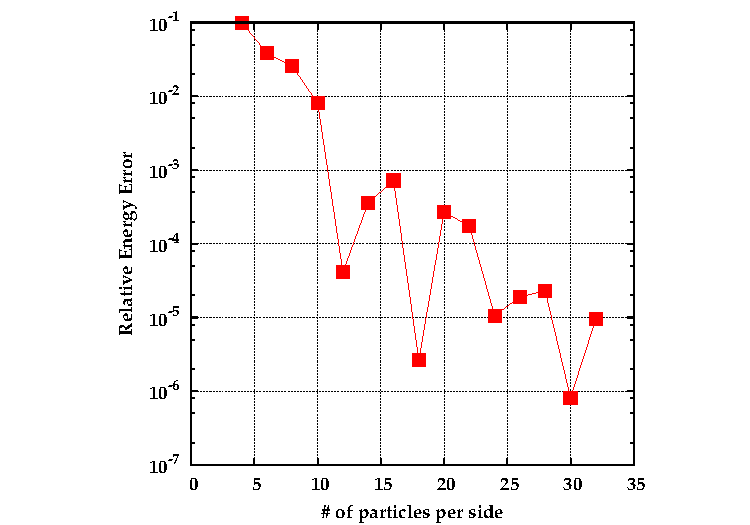
\includegraphics[width=10cm]{fig/p3m.pdf}
\caption{1辺あたりの粒子数とエネルギー相対誤差の関係(メッシュ数は$16^{3}$、カットオフ半径は$3/16$)}
\label{fig:p3m}
\end{figure}
\clearpage

\ifCpp % for C++
%=========================
%   TreePM コードの解説
%=========================
\subsection{TreePMコード} \label{subsec:TreePM}
本節では、FDPSの拡張機能 Particle Mesh (以下、PMと省略する)の使用方法について、TreePM(Tree-Particle-Mesh)法のサンプルコードを用いて解説を行う。このサンプルコードでは、宇宙論的$N$体シミュレーションをTreePM法を用いて実行する。TreePM法は第\ref{subsec:P3M}節で説明した$\mathrm{P^{3}M}$法と同様、重力計算をPPパートとPMパートにsplitして行う。したがって、使用するFDPSの機能は$\mathrm{P^{3}M}$法のサンプルコードとほぼ同じである。2つの方法の違いは、TreePM法ではPPパートの計算を直接法(ダイレクトサム法)ではなくTree法を使って計算する点にある。

\subsubsection{サンプルコードの場所と作業ディレクトリ}
サンプルコードの場所は、\path{$(FDPS)/sample/c++/treepm} である。まずは、そこに移動する。
下に示すように、サンプルコードは複数のファイルから構成される。
この内、FDPSに関係した部分は主に\texttt{treepm.hpp}と\texttt{treepm.cpp}に実装されている。
以下の説明では、適宜、ファイル名を参照していく。
\begin{screen}
\begin{verbatim}
$ cd (FDPS)/sample/c++/treepm
$ ls | awk '{print $0}'
IC/
Makefile
README_en.txt
README_ja.txt
constants.hpp
cosmology.hpp
fig/
make_directory.c
param_file_for_test.txt
prototype.h
result/
run_param.hpp
test.py*
timing.c
treepm.cpp
treepm.hpp
utils/
\end{verbatim}
\end{screen}

\subsubsection{ヘッダファイルのインクルード}
FDPSの標準機能と拡張機能の両方を使うため、メイン関数が定義されたファイル\texttt{treepm.cpp}で、\texttt{particle\_simulator.hpp}と\texttt{particle\_mesh.hpp}をインクルードしている:
\begin{lstlisting}[caption=Include FDPS]
#include <particle_simulator.hpp>
#include <particle_mesh.hpp>
\end{lstlisting}

\subsubsection{ユーザー定義クラス}
FDPSを使用するため、ユーザはユーザ定義クラスを実装しなければならない。
本節では、ユーザ定義クラスをサンプルコードでどのように実装しているかを説明する。

% FullParticle型
\subsubsubsection{FullParticle型}
ユーザーはFullParticle型を記述しなければならない。FullParticle型には、計算を行うにあたり、粒子が持っているべき全ての物理量が含まれている必要がある。Listing \ref{treepm_FP}に、サンプルコードのFullParticle型を示す。このサンプルコードでは通常の$N$体計算に必要なメンバ変数(\texttt{id}, \texttt{mass}, \texttt{eps}, \texttt{pos}, \texttt{vel}, \texttt{acc})に加え、PMパートの加速度を格納する\texttt{acc\_pm}、ハッブル定数を格納する\texttt{H0}、計算領域の大きさを$\mathrm{Mpc\;h^{-1}}$単位で格納する\texttt{Lbnd}が用意されている。また、FDPSの標準機能・拡張機能を使うため、以下のメンバ関数を持たせる必要がある:
\begin{itemize}[leftmargin=*,itemsep=-1ex]
\item \texttt{getCharge()} --- FDPSが粒子の質量を取得するのに必要
\item \texttt{getChargeParticleMesh()} --- FDPSのPMモジュールが粒子の電荷量を取得するために必要
\item \texttt{getPos()} --- FDPSが粒子座標を取得するのに必要
\item \texttt{getRSearch()} --- FDPSがカットオフ半径を取得するのに必要
\item \texttt{setPos()} --- FDPSが粒子の座標を書き込むのに必要
\item \texttt{copyFromForce()} --- Force型から結果をコピーするのに必要なメンバ関数
\item \texttt{copyFromForceParticleMesh()} --- PMモジュールが力の計算結果を書き込むために必要
\end{itemize}
さらに、FDPSの入出力関数を使用するため、以下のメンバ関数を定義してある:
\begin{itemize}[leftmargin=*,itemsep=-1ex]
\item \texttt{readBinary()}
\item \texttt{writeBinary()}
\end{itemize}
但し、この2つは必須ではなく、ユーザ独自の入出力関数を定義してもよい。

\lstinputlisting[linerange={31-222},caption=FullParticle型,label=treepm_FP]{../../../../sample/c++/treepm/treepm.hpp}

% EssentialParticleI型
\subsubsubsection{EssentialParticleI型}
ユーザーはEssentialParticleI型を記述しなければならない。EssentialParticleI型には、PPパートのForce計算を行う際、$i$粒子が持っているべき全ての物理量をメンバ変数として持っている必要がある。Listing \ref{treepm_EPI}に、サンプルコードのEssentialParticleI型を示す。このEssentialParticleI型には、前述したFullParticle型から値をコピーするのに必要なメンバ関数\texttt{copyFromFP()}と、EssentialParticleI型の粒子座標を返すメンバ関数\texttt{getPos()}を持たせる必要がある。

\lstinputlisting[linerange={231-247},caption=EssentialParticleI型,label=treepm_EPI]{../../../../sample/c++/treepm/treepm.hpp}

% EssentialParticleJ型
\subsubsubsection{EssentialParticleJ型}
ユーザーはEssentialParticleJ型を記述しなければならない。\ref{subsec:P3M}節の$\mathrm{P^{3}M}$コードの例では、EssentialParticleJ型はEssentialParticleI型で兼ねていたが、このサンプルコードでは別のクラスとして定義してある。EssentialParticleJ型には、PPパートのForce計算を行う際、$j$粒子が持っているべき全ての物理量をメンバ変数として持っている必要がある。Listing \ref{treepm_EPJ}に、サンプルコードのEssentialParticleJ型を示す。このEssentialParticleJ型には、以下のメンバ関数を持たせる必要がある:
\begin{itemize}[leftmargin=*,itemsep=-1ex]
\item \texttt{getPos()} --- FDPSが粒子位置を取得するのに必要
\item \texttt{getCharge()} --- FDPSが粒子質量を取得するのに必要
\item \texttt{copyFromFP()} --- FDPSがFullParticle型からEssentialParticleJ型に必要な情報を渡すのに必要
\item \texttt{getRSearch()} --- FDPSがカットオフ半径を取得するのに必要
\item \texttt{setPos()} --- FDPSが粒子座標を書き込むのに必要
\end{itemize}

\lstinputlisting[linerange={249-278},caption=EssentialParticleJ型,label=treepm_EPJ]{../../../../sample/c++/treepm/treepm.hpp}

% Force型
\subsubsubsection{Force型}
ユーザーはForce型を記述しなければならない。Force型は、PPパートのForceの計算を行った際にその結果として得られる全ての物理量をメンバ変数として持っている必要がある。本サンプルコードのForce型をListing \ref{treepm_force}に示す。Force型には積算対象のメンバ変数を0ないし初期値に設定するための関数\texttt{clear()}が必要になる。

\lstinputlisting[linerange={19-28},caption=Force型,label=treepm_force]{../../../../sample/c++/treepm/treepm.hpp}

% calcForceEpEp型
\subsubsubsection{calcForceEpEp型}
ユーザーはcalcForceEpEp型を記述しなければならない。calcForceEpEp型には、PPパートのForceの計算の具体的な内容を書く必要がある。サンプルコードのcalcForceEpEp型をListing \ref{treepm_calcForceEpEp}に示す。このサンプルコードでは、calcForceEpEp型はファンクタ(関数オブジェクト)として実装されている(テンプレート関数として実装されていることに注意されたい)。また、Phantom-GRAPEライブラリを使用するかどうかに応じて(マクロ定義\texttt{ENABLE\_PHANTOM\_GRAPE\_X86}で判定している)、場合分けして実装されている。いずれの場合でも、ファンクタの引数は、EssentialParticleIの配列、EssentialParticleIの個数、EssentialParticleJの配列、EssentialParticleJの個数、Force型の配列である。

\lstinputlisting[linerange={344-365},caption=calcForceEpEp型,label=treepm_calcForceEpEp]{../../../../sample/c++/treepm/treepm.hpp}

TreePM法のPPパートは、$\mathrm{P^{3}M}$法と同様、距離に関するカットオフ付きの2体相互作用である。そのため、ここでも加速度計算にカットオフ関数が掛かる。\ref{subsubsubsec:p3m_calcForceEpEp}節で解説したように、カットオフ関数はHockney \& Eastwood (1988)の$S2$型の粒子形状関数に対応したカットオフ関数である必要がある。Phantom-GRAPEライブラリを使用しない場合の実装では、カットオフ関数が関数\texttt{gfactor\_S2()}として定義されている。一方、Phantom-GRAPEライブラリを使用する場合には、カットオフが考慮されたバージョンのPhantom-GRAPEライブラリが使用されるようになっている。Phantom-GRAPEライブラリに指定したカットオフ半径で計算させるため、API \texttt{pg5\_gen\_s2\_force\_table()}を事前に呼び出しておく必要がある。サンプルコードでは、メイン関数でこれを行っている:
\begin{lstlisting}
#ifdef ENABLE_PHANTOM_GRAPE_X86 
    //g5_open();
    pg5_gen_s2_force_table(EPS_FOR_PP, 3.0/SIZE_OF_MESH);
#endif
\end{lstlisting}

% プログラム本体
\subsubsection{プログラム本体}
本節では、サンプルコード本体について解説を行う。詳細な説明に入る前に、サンプルコー ドの内容と全体構造について説明を与える。\ref{subsec:TreePM}節冒頭で述べたように、このサンプルコードでは宇宙論的$N$体シミュレーションをTreePM法を用いて実行する。初期条件としては、以下の3つの場合に対応している:
\begin{enumerate}[leftmargin=*,itemsep=-1ex,label=(\alph*)]
\item Santa Barbara Cluster Comparison Test
  (\href{http://iopscience.iop.org/article/10.1086/307908/meta}{Frenk
  et al.[1999, ApJ, 525, 554]})で用いられた初期条件(以下から初期条件を入手可能。$N=128^3$:
  \href{http://particle.riken.jp/~fdps/data/sb/ic_sb128.tar}{http://particle.riken.jp{\slash}\~{}fdps{\slash}data{\slash}sb{\slash}ic\_sb128.tar}
  、$N=256^3$:
  \href{http://particle.riken.jp/~fdps/data/sb/ic_sb256.tar}{http://particle.riken.jp{\slash}\~{}fdps{\slash}data{\slash}sb{\slash}ic\_sb256.tar})
\item 上記テストで用いられた初期条件ファイルと同じフォーマットで記述された初期条件
\item ランダムにおいた粒子分布
\end{enumerate}
実行時のコマンドライン引数として初期条件を指定した後、初期条件ファイル内で指定された終了時刻(赤方偏移$z$)まで、TreePM法で粒子の運動を計算する。各初期条件に対応したパラメータファイルのファイルフォーマットについては、\path{$(FDPS)/sample/c++/treepm/README_ja.txt} で説明されているので、そちらを参照されたい。また、\path{$(FDPS)/sample/c++/treepm/result/input.para} に、(a)の場合のパラメータファイルの記述例があるので、そちらも参照されたい。

コード全体の構造は以下のようになっている:
\begin{enumerate}[leftmargin=*,itemsep=-1ex,label=(\arabic*)]
\item FDPSで使用するオブジェクトの生成と初期化
\item (必要であれば)Phantom-GRAPEライブラリの初期化
\item 初期条件ファイルの読み込み
\item 終了時刻まで粒子の運動を計算
\end{enumerate}

以下で、個々について詳しく説明を行う。

\subsubsubsection{開始、終了}
まずは、FDPSの初期化/開始を行う必要がある。
次のように、メイン関数に記述する。
\begin{lstlisting}[caption=FDPSの開始]
PS::Initialize(argc, argv);
\end{lstlisting}

FDPSは、開始したら明示的に終了させる必要がある。
今回は、プログラムの終了と同時にFDPSも終了させるため、メイン関数の最後に次のように記述する。
\begin{lstlisting}[caption=FDPSの終了]
PS::Finalize();
\end{lstlisting}

\subsubsubsection{オブジェクトの生成と初期化}
FDPSの初期化に成功した場合、ユーザーはコード中で用いるオブジェクトを作成する必要がある。
本節では、オブジェクトの生成/初期化の仕方について、解説する。

\subsubsubsubsection{オブジェクトの生成}
TreePM法の計算では、$\mathrm{P^{3}M}$法のときと同様、粒子群クラス、領域クラス、PPパートの計算で使用するtreeを1本、そして、PMパートの計算に必要なParticleMeshオブジェクトの生成が必要である。本サンプルコードでは、\texttt{treepm.cpp}のメイン関数内でオブジェクトの生成が行われている:
\begin{lstlisting}[caption=オブジェクトの生成]
int main(int argc, char **argv)
{
   PS::PM::ParticleMesh pm;
   PS::ParticleSystem<FPtreepm> ptcl;
   PS::DomainInfo domain_info;
   PS::TreeForForceLong<Result_treepm, EPItreepm, EPJtreepm>::MonopoleWithCutoff treepm_tree;
}
\end{lstlisting}
上記はサンプルコードからオブジェクト生成部分だけを抜き出してきたものであることに注意されたい。

\subsubsubsubsection{オブジェクトの初期化}
ほとんどのFDPSのオブジェクトは、生成後、初期化してから使用する必要がある。前節で説明した4つのオブジェクトの内、明示的な初期化が不要なのはParticleMeshクラスである。それ以外のオブジェクトに関しては、\texttt{initialize}メソッドで初期化を行う。以下に、サンプルコードでのオブジェクトの初期化を示す:
\begin{lstlisting}[caption=オブジェクトの初期化]
int main(int argc, char **argv)
{
   // Initialize ParticleSystem
   ptcl.initialize();

   // Initialize DomainInfo
   domain_info.initialize();  
   domain_info.setBoundaryCondition(PS::BOUNDARY_CONDITION_PERIODIC_XYZ);
   domain_info.setPosRootDomain(PS::F64vec(0.0, 0.0, 0.0), 
                                PS::F64vec(1.0, 1.0, 1.0));
                                
   // Initialize Tree
   treepm_tree.initialize(3*ptcl.getNumberOfParticleGlobal(),
                          this_run.theta);
}
\end{lstlisting}

粒子群クラスのオブジェクトの初期化は、単に\texttt{initialize}メソッドを引数無しで呼び出すだけである。


領域クラスに関しては、\texttt{initialize}メソッド呼び出し後に、境界条件と境界の大きさを指定する必要がある。
これらはそれぞれ\texttt{setBoundaryCondition}メソッドと\texttt{setPosRootDomain}メソッドで行う。

ツリーオブジェクトの初期化の際には、\texttt{initialize}メソッドに計算で使用する大雑把な粒子数を第1引数として渡す必要がある。本サンプルコードでは、全粒子数の3倍の値を渡している。第2引数には、tree法で力の計算を行う際のopening angle criterion $\theta$を指定する。本サンプルコードでは、$\theta$をはじめとした、計算を制御するパラメータ群を構造体\texttt{this\_run}のメンバ変数としてまとめている。


\subsubsubsection{初期条件の設定}
初期条件を指定するパラメータファイルの読み込みは、メイン関数で呼ばれる関数\texttt{read\_param\_file()}内で行われる:
\begin{lstlisting}
read_param_file(ptcl, this_run, argv[1]);
\end{lstlisting}
この関数ではプログラム実行時に指定されたパラメータファイルを読み込み、粒子群クラスのオブジェクト\texttt{ptcl}に粒子データをセットする。サンプルコードでは、この後、FDPSのAPIを使って、領域分割と粒子交換を行っている。以下でこれらのAPIについて解説する。

\subsubsubsubsection{領域分割の実行}
粒子分布に基いて領域分割を実行するには、領域クラスの\texttt{decomposeDomainAll}メソッドを使用する:
\begin{lstlisting}[caption=領域分割の実行]
domain_info.decomposeDomainAll(ptcl);
\end{lstlisting}
ここで、粒子分布の情報を領域クラスに与えるため、引数に粒子群クラスのオブジェクトが渡されていることに注意されたい。
この領域分割はメイン関数内で行われている。


\subsubsubsubsection{粒子交換の実行}
領域情報に基いてプロセス間の粒子の情報を交換するには、粒子群クラスの\texttt{exchangeParticle}メソッドを使用する:
\begin{lstlisting}[caption=粒子交換の実行]
ptcl.exchangeParticle(domain_info);
\end{lstlisting}
ここで領域情報を粒子群クラスに与えるため、引数に領域クラスのオブジェクトが渡されていることに注意する。

\subsubsubsection{相互作用計算の実行}
領域分割・粒子交換が完了したら、計算開始時の加速度を決定するため、相互作用計算を行う必要がある。
以下に、本サンプルコードでの相互作用計算の実装を示す。
本サンプルコードでは、PPパートの計算にはツリーオブジェクトの\texttt{calcForceAllAndWriteBack}メソッドを使用している。
このメソッドを実行することで、粒子群オブジェクトのメンバ変数\texttt{acc}にPPパートの加速度が格納される。
PMパートの計算にはParticleMeshオブジェクトの\texttt{calcForceAllAndWriteBack}メソッドを使用している。
これによって、粒子群クラスのメンバ変数\texttt{acc\_pm}にPMパートの加速度が格納される。

\begin{lstlisting}[caption=相互作業計算の実行]
//* PP part
treepm_tree.calcForceAllAndWriteBack
    (calc_pp_force<EPJtreepm>(),
     calc_pp_force<PS::SPJMonopoleCutoff>(),
     ptcl,
     domain_info);
 
//* PM part
pm.calcForceAllAndWriteBack(ptcl, domain_info); 
\end{lstlisting}

\subsubsubsection{時間積分ループ}
本サンプルコードでは、時間積分をLeapfrog時間積分法によって行っている(この方法に関しては、\ref{s4sec:nbody_time_integration}節を参照されたい)。粒子位置を時間推進する$D(\cdot)$オペレータは関数\texttt{drift\_ptcl}、粒子速度を時間推進する$K(\cdot)$オペレータは関数\texttt{kick\_ptcl}として実装されている。宇宙膨張の効果は関数\texttt{kick\_ptcl}内で考慮されている。また、スケールファクターやハッブルパラメータの時間発展は構造体\texttt{this\_run}のメンバ関数\texttt{update\_expansion}で計算されている。

\subsubsection{コンパイル}
README.txtで説明されているように、Makefileを適宜編集し、\texttt{make}コマンドを実行することでコンパイルすることができる。$\mathrm{P^{3}M}$コード同様、本サンプルコードでもFFTWライブラリを使用するため、ユーザ自身でインストールする必要がある。コンパイルが成功すれば、実行ファイル\texttt{treepm}が作成されているはずである。

\subsubsection{実行}
FDPSの拡張機能ParticleMeshの仕様上、プロセス数が2以上のMPI実行でなければ正常に動作しない。
そこで、以下のように実行する必要がある:
\begin{screen}
\begin{verbatim}
$ MPIRUN -np NPROC ./treepm
\end{verbatim}
\end{screen}
ここで、"MPIRUN"にはmpirunやmpiexecなどのMPI実行プログラムが、"NPROC"にはプロセス数が入る。

\subsubsection{結果の確認}
計算が終了するとパラメータファイルで指定されたディレクトリに計算結果が出力されるはずである。
粒子数$256^{3}$で、Santa Barbara Cluster Comparison Testを実行した場合の、ダークマター密度分布の時間発展の様子を図\ref{fig:treepm}に示す。

\begin{figure}[h]
\centering
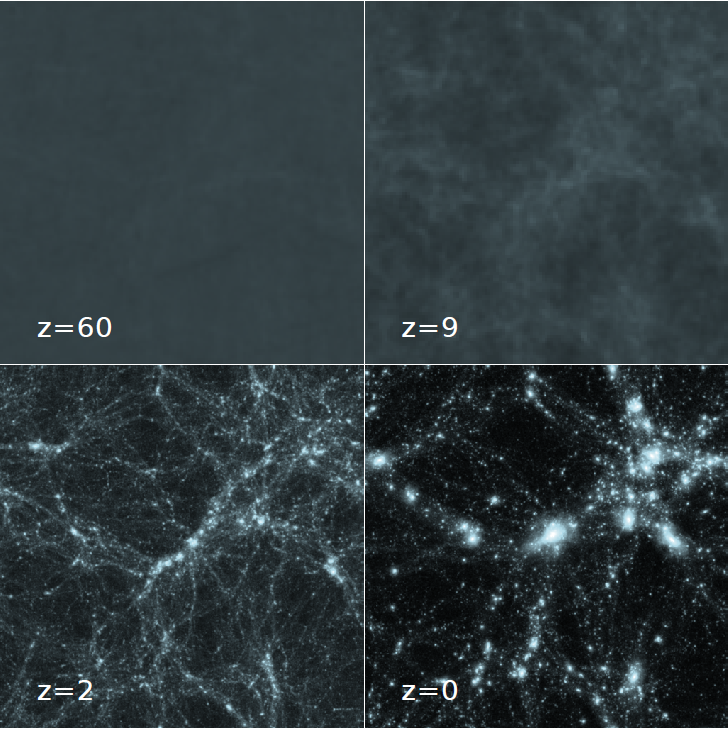
\includegraphics[width=0.666\linewidth]{./fig/sb256.png}
\caption{Santa Barbara Cluster Comparison テストの密度分布の時間発展(粒子数$256^{3}$)}
\label{fig:treepm}
\end{figure}

\endifCpp % \ifCpp はTreePMコードの節全体に掛かっている.
\clearpage

%%%%%%%%%%%%%%%%%%%%%%%%%%%%%%%%%%%%%%%%%%%%%%%%%%%%%
\section{より実用的なアプリケーションの解説}
\label{sec:applications}
In previous sections, we have explained fundamental features of FDPS using relatively simple application codes. However, we need to develop a more complex application in actual research, in which for example we need to treat different types of particles. In this section, we will explain advanced features of FDPS using practical applications. \ul{To keep the explanations short and simple, we require the readers understand the contents of the previous sections in this document}.
%=============================
%   N-body+SPH code
%=============================
\subsection{$N$-body/SPH code} \label{subsec:NbodySPH}
In this section, we explain the accompanying sample code for $N$-body/SPH simulation of a disk galaxy. In this code, dark matter and stars, which perform gravitational interaction only, are represented by $N$-body particles, while interstellar gas, which performs both gravitational and hydrodynamic interactions, is represented by SPH particles. The tree method is used for the gravity calculation. The SPH scheme adopted in this code is the one proposed by \href{https://doi.org/10.1046/j.1365-8711.2002.05445.x}{Springel \& Hernquist [2002, MNRAS, 333, 649]} and \href{https://doi.org/10.1111/j.1365-2966.2005.09655.x}{Springel [2005, MNRAS, 364, 1105]} (hereafter, we call it Springel's SPH scheme). The readers can understand how to treat different types of particles using FDPS by reading this section.

Below, we first explain the usage of the code. Next, we give a brief explanation of the Springel's SPH scheme. Then, we explain the contents of the sample source codes in detail.

\subsubsection{How to run the sample code}
\label{subsubsec:NbodySPH_usage}
As we described, this code simulates the dynamical evolution of a disk galaxy. This code sets the initial distributions of dark matter and stars by reading a file created by \href{https://bitbucket.org/ymiki/magi}{\textsc{MAGI}} (\href{https://doi.org/10.1093/mnras/stx3327}{Miki \& Umemura [2018, MNRAS, 475, 2269]}), which is a software to make an initial condition of a galaxy simulation. On the other hand, the initial gas distribution is set inside the code. Therefore, the following procedures are required to use the code.
\begin{itemize}
\item Move to directory \dirNameNbodySPHSample
\item Edit \texttt{Makefile} in the current directory
\item Create particle data using \href{https://bitbucket.org/ymiki/magi}{\textsc{MAGI}} and place it under directory\texttt{./magi\_data/dat}
\item Run the \texttt{make} command to create the executable \texttt{nbodysph.out}
\item Run \texttt{nbodysph.out}
\item Check the output
\end{itemize}

Below, we explain each procedure.

\subsubsubsection{Move to the directory the sample code is placed}
\label{s3sec:NbosySPH_code_loc}
Move to \dirNameNbodySPHSample.

\subsubsubsection{File structure of the sample code}
\label{s3sec:NbodySPH_file_str}
The following is the file structure of the sample code.
\ifCpp % for C++
\begin{screen}
\begin{verbatim}
$ ls | awk '{print $0}'
Makefile
Makefile.K
Makefile.ofp
ic.hpp
job.K.sh
job.ofp.sh
leapfrog.hpp
macro_defs.hpp
magi_data/
main.cpp
mathematical_constants.cpp
mathematical_constants.h
physical_constants.cpp
physical_constants.h
test.py*
user_defined.hpp
\end{verbatim}
\end{screen}
We explain briefly the content of each source file. In \texttt{ic.hpp}, functions to create initial conditions are implemented. Users can choose an initial condition other than that for a disk galaxy (described later). In \texttt{leapfrog.hpp}, we implement functions necessary to integrate the orbits of particles based on the Leapfrog method. In \texttt{macro\_defs.hpp}, we define macros that are used to control numerical simulation. In \texttt{main.cpp}, the main routine is implemented. In \texttt{mathematical\_constants.h} and \texttt{mathematical\_constants.cpp}, we define some mathematical constants. In \texttt{physical\_constants.h} and \texttt{physical\_constants.cpp}, we define some physical constants. In \texttt{user\_defined.hpp}, we define user-defined classes and interaction functions.
\endifCpp
\ifFtn % for Fortran
\begin{screen}
\begin{verbatim}
$ ls | awk '{print $0}'
Makefile
Makefile.K
Makefile.intel
Makefile.ofp
f_main.F90
ic.F90
job.K.sh
job.ofp.sh
leapfrog.F90
macro_defs.h
magi_data/
mathematical_constants.F90
physical_constants.F90
test.py
tipsy_file_reader.cpp
tipsy_file_reader.h
user_defined.F90
\end{verbatim}
\end{screen}
We explain briefly the content of each source file. In \texttt{ic.F90}, subroutines to create initial conditions are implemented. Users can choose an initial condition other than that for a disk galaxy (described later). In \texttt{leapfrog.F90}, we implement subroutines necessary to integrate the orbits of particles based on the Leapfrog method. In \texttt{macro\_defs.h}, we define macros that are used to control numerical simulation. In \texttt{f\_main.F90}, the main routine is implemented. In \texttt{mathematical\_constants.F90}, we define some mathematical constants. In \texttt{physical\_constants.F90}, we define some physical constants. In \texttt{tipsy\_file\_reader.*}, we define functions to read particle data created by \textsc{MAGI}. In \texttt{user\_defined.F90}, we define user-defined types and interaction functions.
\endifFtn
\ifC % for C
\begin{screen}
\begin{verbatim}
$ ls | awk '{print $0}'
Makefile
Makefile.ofp
c_main.c
ic.c
ic.h
job.ofp.sh
leapfrog.c
leapfrog.h
macro_defs.h
magi_data/
mathematical_constants.c
mathematical_constants.h
physical_constants.c
physical_constants.h
tipsy_file_reader.cpp
tipsy_file_reader.h
user_defined.c
user_defined.h
\end{verbatim}
\end{screen}
We explain briefly the content of each source file. In \texttt{ic.*}, functions to create initial conditions are implemented. Users can choose an initial condition other than that for a disk galaxy (described later). In \texttt{leapfrog.*}, we implement functions necessary to integrate the orbits of particles based on the Leapfrog method. In \texttt{macro\_defs.h}, we define macros that are used to control numerical simulation. In \texttt{c\_main.c}, the main function is implemented. In \texttt{mathematical\_constants.*}, we define some mathematical constants. In \texttt{physical\_constants.*}, we define some physical constants. In \texttt{tipsy\_file\_reader.+}, we define functions to read particle data created by \textsc{MAGI}. In \texttt{user\_defined.*}, we define user-defined types and interaction functions.
\endifC

Directory \texttt{magi\_data} stores a parameter file input to the software \textsc{MAGI} (\texttt{magi\_data/cfg/*}) and a script file used to run \textsc{MAGI} (\texttt{magi\_data/sh/run.sh}).

\subsubsubsection{Edit Makefile}
\label{s3sec:NbodySPH_Makefile}
Edit \path{Makefile} following the description below.
\begin{itemize}
\item Set the variable \path{CXX} the command to run your C++ compiler.
\ifFtn % for Fortran
\item Set the variable \path{FC} the command to run your Fortran compiler.
\endifFtn
\ifC % for C
\item Set the variable \path{CC} the command to run your C compiler.
\endifC
\item Set the variable \path{CXXFLAGS} compile options of the C++ compiler.
\ifFtn % for Fortran
\item Set the variable \path{FCFLAGS} compile options of the Fortran compiler.
\endifFtn
\ifC % for C
\item Set the variable \path{CFLAGS} compile options of the C compiler.
\endifC
\item In this code, several macros are used to control numerical simulations. Table \ref{tbl:NbodySPH:compile_time_macros} lists the names of the macros and their definitions. In addition, there are macros whose states (i.e. value or defined/undefined states) are automatically set according to the value of macro \path{INITIAL_CONDITION}. Generally, users do not have to change them. Please see \path{macro_defs.h} directly for detail.
\item Phantom-GRAPE library for x86 can be used for the gravity calculation. To use it, set the variable \path{use_phantom_grape_x86} \path{yes}.
\end{itemize}
As for the way to specify the use/non-use of OpenMP and MPI, see \S~\ref{sec:getting_started}.


\begin{table}[H]
\begin{tabularx}{\linewidth}{|c|X|}
\toprule
\rowcolor{Snow2}
Macro name & Defintion \\
\midrule
\path{INITIAL_CONDITION} & It specifies the type of initial condition or the operation mode of the code. It must take a value from 0 to 3. According to its value, the code operates as follows. 0: an initial condition for a disk galaxy is used, 1: an initial condition for cold collapse test problem is used, 2: an initial condition for Evrard test is used, 3: the code operates in the mode to make a glass-like distribution of SPH particles. \\
\midrule
\path{ENABLE_VARIABLE_SMOOTHING_LENGTH} & It specifies that smoothing length of SPH particles is variable or not. If it is defined, variable smoothing length is used and the SPH calculation is performed according to the Springel's SPH scheme. If it is not defined, the fixed smoothing length is used and the SPH calculation is done in almost the same way as the sample code described in \S~\ref{sec:getting_started}-\ref{sec:how_to_use}. \\
\midrule
\path{USE_ENTROPY} & It specifies whether to use entropy or specific internal energy as an independent variable to describe the thermodynamic state of SPH particle. If defined, entropy is used. But, if macro \path{ISOTHERMAL_EOS} described below is defined, specific internal energy is forcibly used (specific internal energy is used to calculate pressure). \\
\midrule
\path{USE_BALSARA_SWITCH} & It specifies whether Balsara switch (\href{https://doi.org/10.1016/S0021-9991(95)90221-X}{Balsara [1995, JCP, 121, 357]}) is used or not. If defined, the Balsara switch is used. \\ 
\midrule
\path{USE_PRESCR_OF_THOMAS_COUCHMAN_1992} & It specifies whether a simple prescription proposed by \href{https://doi.org/10.1093/mnras/257.1.11}{Thomas \& Couchman [1992, MNRAS,257, 11]} to prevent the tensile instability is used or not. If defined, this prescription is used. \\
\midrule
\path{ISOTHERMAL_EOS} & It specifies whether isothermal process is assumed or not. If defined, isothermal process is assumed (specific internal energy is assumed to be constant). If not defined, the code solve the entropy equation or the internal energy equation.\\
\midrule
\path{READ_DATA_WITH_BYTESWAP} & It specifies whether the program reads particle data with performing byte swap (byte swap is applied for each variable of basic data type). If defined, byte swap is performed.\\
\bottomrule
\end{tabularx}
\caption{Compile-time macros and their definitions}
\label{tbl:NbodySPH:compile_time_macros}
\end{table}

\subsubsubsection{Create particle data using MAGI}
\label{s3sec:NbodySPH_MAGI_usage}
As described earlier, users need to create particle data using the software \textsc{MAGI} before simulation according to the procedures described below. For users who cannot use \texttt{MAGI} for some reasons, we prepared sample particle data in web sites described below. In the following, we explain each case in detail.
\begin{description}
\item[Create particle data using \textsc{MAGI}] Create particle data as follows.
\begin{enumerate}
\item Download the source file of \textsc{MAGI} from the web side \href{https://bitbucket.org/ymiki/magi}{https://bitbucket.org{\slash}ymiki{\slash}magi} and install it in appropriate PATH according to the descriptions in Section ``How to compile MAGI" in the above web side. \ul{But, our {$N$}-body/SPH sample code supports TIPSY file format only. Therefore, please build {\textsc{MAGI}} with {\path{USE_TIPSY_FORMAT=ON}}}.
\item Edit \texttt{./magi\_data/sh/run.sh} and set the variable \path{MAGI_INSTALL_DIR} the PATH of the directory where the \texttt{magi} command is stored. Also, set the variable \texttt{NTOT} the number of $N$-body particles (\textsc{MAGI} automatically assigns the numbers of dark matter particles and star particles).
\item Edit \texttt{./magi\_data/cfg/*} to specify a galaxy model. For detail of the format of input file for \textsc{MAGI}, please see the web side above or Section 2.4 in the original paper \href{https://doi.org/10.1093/mnras/stx3327}{Miki \& Umemura [2018, MNRAS, 475, 2269]}. In the default, galaxy model consists of the following four components (hereafter, we call this \textbf{default galaxy model}):
\begin{enumerate}[label=(\roman*)]
\item Dark matter halo (NFW profile, $M=10^{12}\;\mathrm{M_{\odot}}$, $r_{s}=21.5\;\mathrm{kpc}$, $r_{c}=200\;\mathrm{kpc}$, $\Delta_{c}=10\;\mathrm{kpc}$)
\item Stellar bulge (King model, $M=5\times 10^{10}\;\mathrm{M_{\odot}}$, $r_{s}=0.7\;\mathrm{kpc}$, $W_{0}=5$)
\item Thick stellar disk  (S{\'e}rsic profile, $M=2.5\times 10^{10}\;\mathrm{M_{\odot}}$, $r_{s}=3.5\;\mathrm{kpc}$, $n=1.5$, $z_{d}=1\;\mathrm{kpc}$, $Q_{T,\min}=1.0$)
\item Thin stellar disk (exponential disk, $M=2.5\times 10^{10}\;\mathrm{M_{\odot}}$, $r_{s}=3.5\;\mathrm{kpc}$, $z_{d}=0.5\;\mathrm{kpc}$, $Q_{T,\min}=1.0$)
\end{enumerate}
In the default galaxy model, two stellar disks are marginally unstable to a bar-mode in view of the Ostriker-Peebles criterion. Therefore, a simulated galaxy is expected to evolve into a spiral galaxy having a weak bar. In the latest release of \textsc{MAGI} (version 1.1.1 [as of July 19th, 2019]), its default operation mode is changed from previous releases. With this demand, we have replaced parameter $f$ in thick and thin disks by $Q_{T,\min}$, where $f$ is a parameter controlling the velocity dispersion of disk and is used in the previous releases of \textsc{MAGI} to specify the stability of a disk component. $Q_{T,\min}$ is the minimum of Toomre Q value in the disk. (In the sample code in FDPS 5.0d or earlier, we used $f=0.125$).
\item Move to directory \texttt{magi\_data} and run the following command:
\begin{screen}
\$ ./sh/run.sh
\end{screen}
\item If \textsc{MAGI} stops successfully, particle data whose extension is \texttt{tipsy} will be created in directory \path{magi_data/dat}.
\end{enumerate}
\item[Download sample particle data form our web sites]  Download a particle data file from one of the following URLs and place it under directory \texttt{./magi\_data/dat/}. All of particle data is made with the default galaxy model. Only the number of particles is different for each data.
\begin{itemize}
\item $N=2^{21}$: \url{https://v2.jmlab.jp/owncloud/index.php/s/XnzvW5XAYwfqZYQ/download?path=%2Fmagi_data%2FGalaxy%2F21&files=Galaxy.tipsy}
\item $N=2^{22}$: \url{https://v2.jmlab.jp/owncloud/index.php/s/XnzvW5XAYwfqZYQ/download?path=%2Fmagi_data%2FGalaxy%2F22&files=Galaxy.tipsy}
\item $N=2^{23}$: \url{https://v2.jmlab.jp/owncloud/index.php/s/XnzvW5XAYwfqZYQ/download?path=%2Fmagi_data%2FGalaxy%2F23&files=Galaxy.tipsy}
\item $N=2^{24}$: \url{https://v2.jmlab.jp/owncloud/index.php/s/XnzvW5XAYwfqZYQ/download?path=%2Fmagi_data%2FGalaxy%2F24&files=Galaxy.tipsy}
\end{itemize}
\end{description}

\subsubsubsection{Run make}
\label{s3sec:NbodySPH_make}
Type ``make'' to run the \path{make} command.

\subsubsubsection{Run the sample code}
\label{s3sec:NbodySPH_execution}
\begin{itemize}
\item If you are not using MPI, run the following in CLI (terminal)
\begin{screen}
\begin{verbatim}
$ ./nbodysph.out
\end{verbatim}
\end{screen}
  
\item If you are using MPI, run the following in CLI (terminal)
\begin{screen}
\begin{verbatim}
$ MPIRUN -np NPROC ./nbodysph.out
\end{verbatim}
\end{screen}
where \texttt{MPIRUN} should be \texttt{mpirun} or \texttt{mpiexec} depending on your MPI configuration, and \texttt{NPROC} is the number of processes you will use.
\end{itemize}

\subsubsubsection{Analysis of the result}
\label{s3sec:NbodySPH_result_analysis}
\ifCpp % for C++
In the directory \path{result}, data of $N$-body and SPH particles are output as files ``nbody0000x.dat" and ``sph0000x.dat", where x is an integer representing time.
\endifCpp
\ifIF % for Fortran and C
In the directory \path{result}, data of $N$-body and SPH particles are output as files ``nbody0000x-proc0000y.dat" and ``sph0000x-proc0000y.dat", where x is an integer representing time and y is an integer representing a process number (MPI rank number).
\endifIF
The output file format of $N$-body particle data is that in each line, index of particle, mass, position (x, y, z), velocity (vx, vy, vz) are listed. The output file format of SPH particle data is that in each line, index of particle, mass, positon (x, y, z), velocity (vx, vy, vz), density, specific internal energy, entropy, pressure are listed.

Figure~\ref{fig:nbodysph} shows the distribution of star and SPH particles at $T=0.46$ for a disk galaxy simulation with the number of $N$-body particles is $2^{21}$ and the number of SPH particles is $2^{18}$.

\begin{figure}[h]
\centering
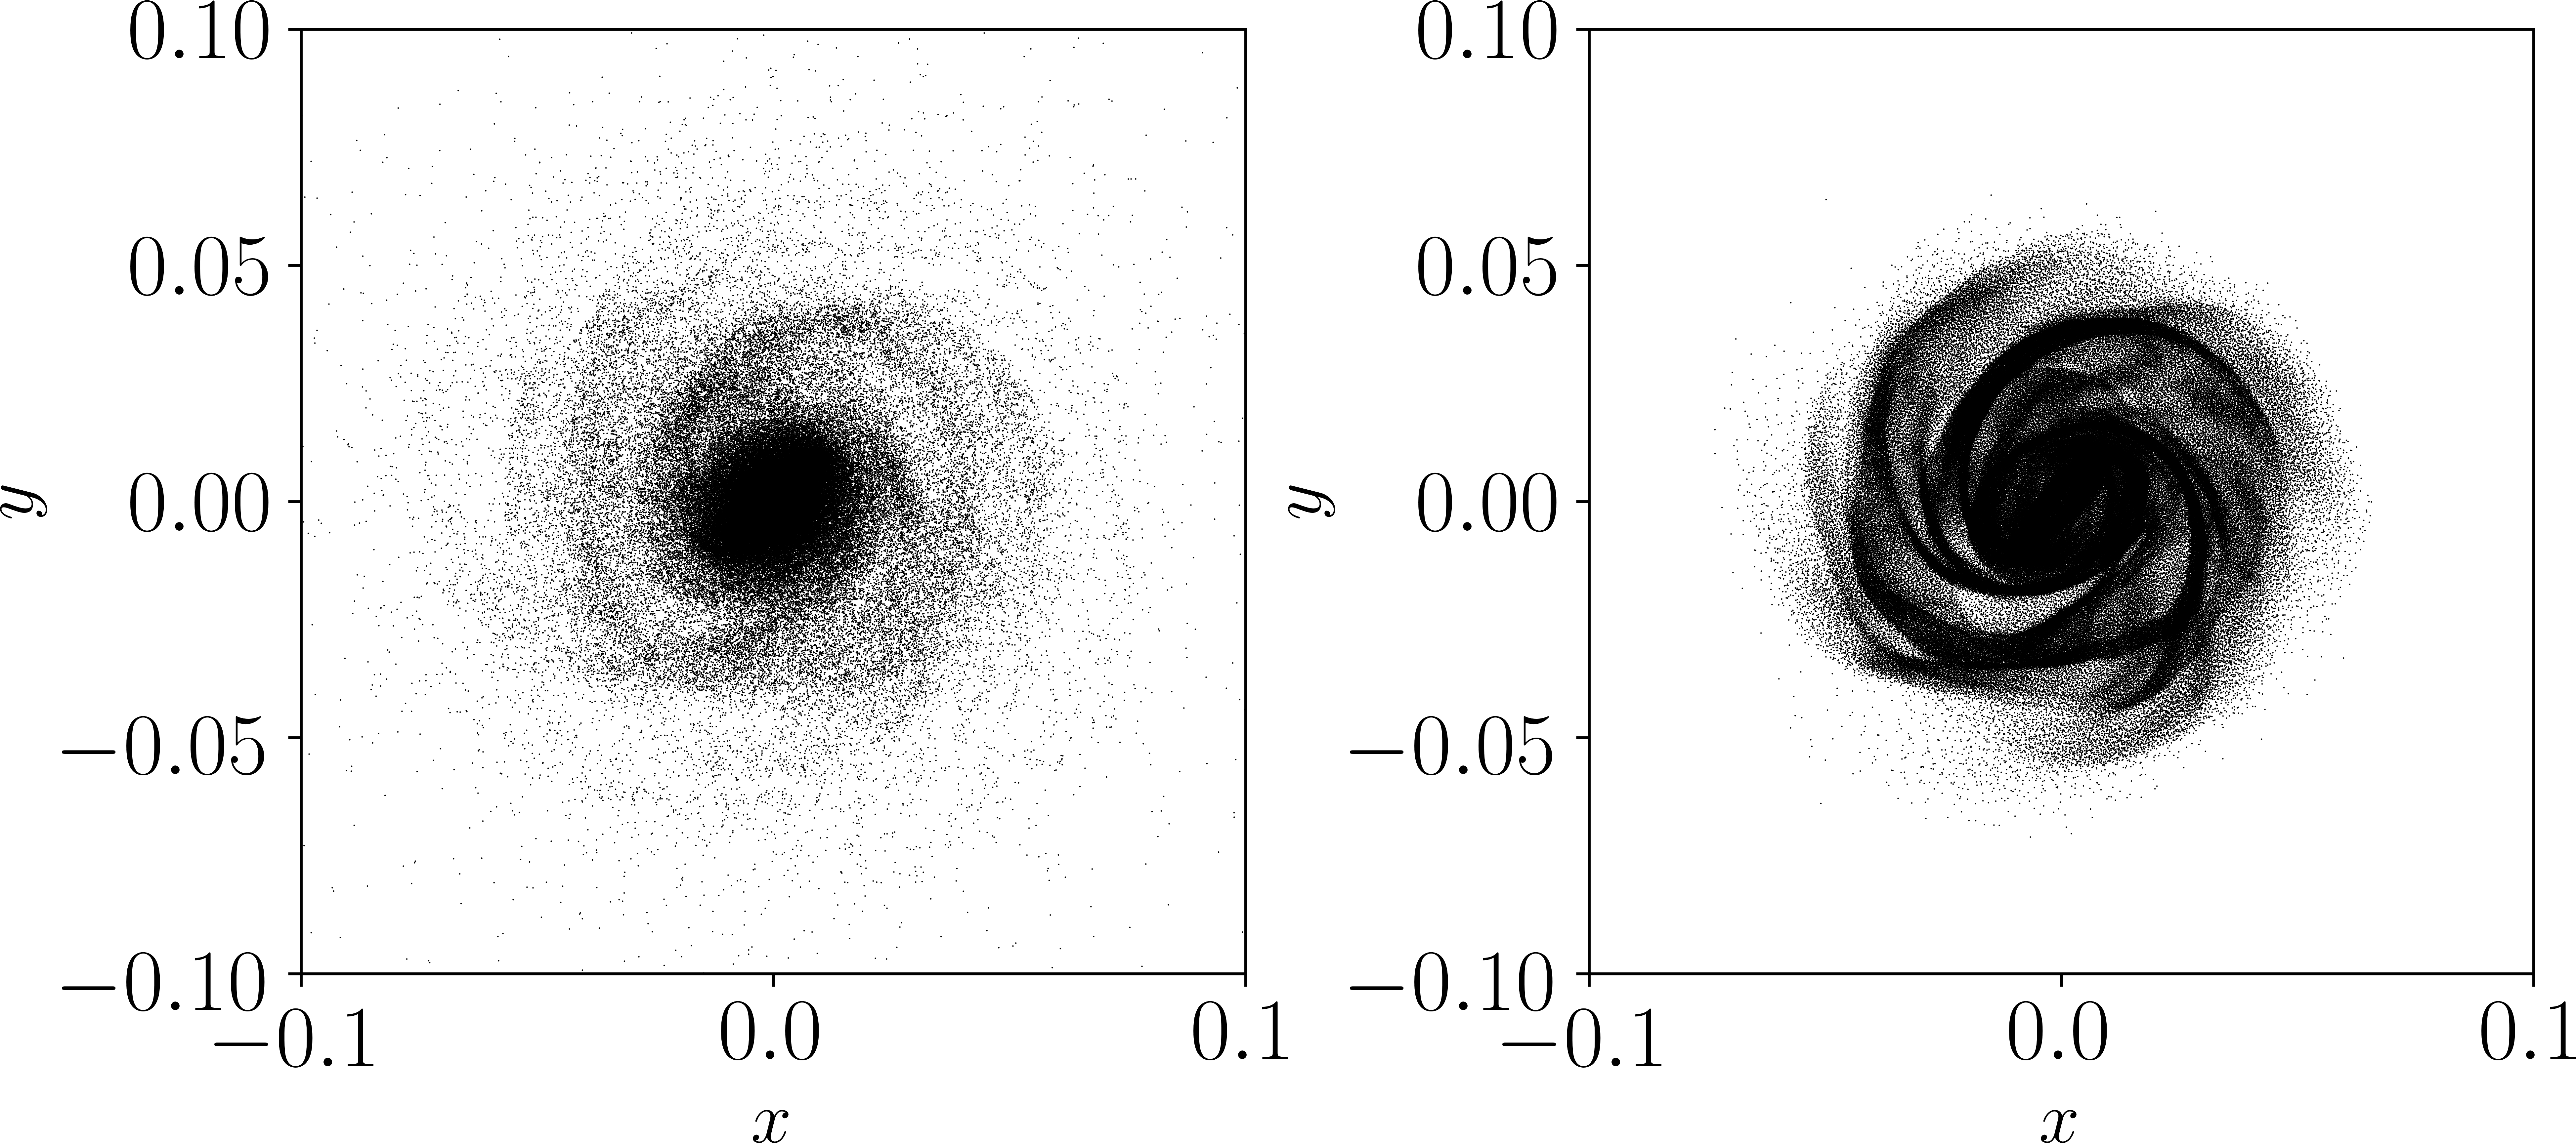
\includegraphics[width=\linewidth]{./fig/nbodysph_t046.png}
\caption{Face-on view of distributions of stars (left) and gas (right) (simulation configuration: the simulation is performed the number of $N$-body particles is $2^{21}$, the number of SPH particles is $2^{18}$, isothermal, gas temperature is $10^{4}\;\mathrm{K}$, mean molecular weight to the mass of hydrogen $\mu=0.5$)}
\label{fig:nbodysph}
\end{figure}


Below, we briefly explain the Springel's SPH scheme and then explain the implementation of the sample code.


\subsubsection{Springel's SPH scheme}
\label{subsubsec:Springel_scheme}
\href{https://doi.org/10.1046/j.1365-8711.2002.05445.x}{Springel \& Hernquist [2002, MNRAS, 333, 649]} proposed a formulation of SPH (actually, equation of motion[EoM]) where the total energy and entropy of a system are conserved even if smoothing length changes with time. In this section, we briefly explain their formulation. The outline of the derivation is as follows. Construct a Lagrangian of the system assuming that smoothing length is also independent variable, then solve the Euler-Lagrange equations under $N$ constraints, where $N$ is the number of particles.

More specifically, they consider the Lagrangian
\begin{equation}
L(\bm{q}, \dot{\bm{q}}) = \dfrac{1}{2}\sum^{N}_{i=1}m_{i}\dot{\bm{r}}^{2}_{i} - \dfrac{1}{\gamma -1}\sum^{N}_{i=1}m_{i}A_{i}\rho^{\gamma-1}_{i} \label{eq:Lagrangian}
\end{equation}
where $\bm{q}=(\bm{r}_{1},...,\bm{r}_{N},h_{1},...h_{N})$ is the generalized coordinates (the subscripts represent the indice of particles), $\bm{r}_{i}$ is the position, $h_{i}$ is smoothing length, $m_{i}$ is mass, $\gamma$ is the ratio of specific heats, $\rho_{i}$ is density, $A_{i}$ is called entropy function and it is related with specific internal energy $u_{i}$ and $\rho_{i}$ through the equation
\begin{equation}
u_{i} = \dfrac{A_{i}}{\gamma-1}\rho^{\gamma-1}_{i} \label{eq:relation_between_u_A_rho}
\end{equation}
The first and second terms of Eq.(\ref{eq:Lagrangian}) represents the kinetic energy and the internal energy of the system, respectively. Because solving the Euler-Lagrangian equation directly using this Lagrangian results in $4N$ equations, which is not undesirable, they introduce the following $N$ constraints.
\begin{equation}
\phi_{i} = \dfrac{4\pi}{3}h^{3}_{i}\rho_{i} - \overline{m}N_{\mathrm{neigh}}=0 \label{eq:Springel_SPH_constraints}
\end{equation}
where $\overline{m}$ is the average mass of SPH particles\footnote{This must be treated as constant.}, $N_{\mathrm{neigh}}$ is the number of neighbor particles (constant). Under these constraints, using the method of Lagrange multiplier, they solve the Euler-Lagrange equations to obtain the following equations of motion:
\begin{equation}
\dfrac{\mathrm{d}\bm{v}_{i}}{\mathrm{d}t} = - \sum^{N}_{j=1}m_{j}\left[f_{i}\dfrac{P_{i}}{\rho^{2}_{i}}\nabla_{i}W(r_{ij},h_{i})+f_{j}\dfrac{P_{j}}{\rho^{2}_{j}}\nabla_{i}W(r_{ij},h_{j})\right] \label{eq:Springel_SPH_EoM_pure_hydro}
\end{equation}
where $P_{i}$ is pressure, $r_{ij}=|\bm{r}_{i}-\bm{r}_{j}|$, $W$ is the kernel function, $f_{i}$ is the so-called $\nabla h$ term, defined by
\begin{equation}
f_{i} = \left(1 + \dfrac{h_{i}}{3\rho_{i}}\dfrac{\partial \rho_{i}}{\partial h_{i}}\right)^{-1} \label{eq:gradh_term}
\end{equation}

The thermodynamic state of the system is described by the independent variable $A_{i}$, the entropy. If the flow is adiabatic, the entropy is constant along the flow except for locations of shock waves where the entropy is increased. \href{https://doi.org/10.1111/j.1365-2966.2005.09655.x}{Springel [2005, MNRAS, 364, 1105]} modeled the increase of the entropy by passing shock waves using the method of artificial viscosity:
\begin{align}
\dfrac{\mathrm{d}A_{i}}{\mathrm{d}t} & = \dfrac{1}{2}\dfrac{\gamma-1}{\rho^{\gamma-1}_{i}}\sum^{N}_{j=1}m_{j}\Pi_{ij}\bm{v}_{ij}\cdot\nabla_{i}\overline{W}_{ij} \label{eq:Springel_SPH_entropy_eq} \\
\left.\dfrac{\mathrm{d}\bm{v}_{i}}{\mathrm{d}t}\right|_{\mathrm{visc}} & = -\sum^{N}_{j=1}m_{j}\Pi_{ij}\nabla_{i}\overline{W}_{ij} \label{eq:Springel_SPH_EoM_art_vis}
\end{align}
where $\bm{v}_{ij}=\bm{v}_{i}-\bm{v}_{j}$, $\bm{v}_{i}$ is velocity, $\overline{W}_{ij}=\frac{1}{2}(W(r_{ij},h_{i})+W(r_{ij},h_{j}))$. For $\Pi_{ij}$, please see the original papers.

The procedures of SPH calculation is summarized as follows:
\begin{screen}
\begin{enumerate}[leftmargin=*,itemsep=-1ex,label={(\arabic*)}]
\item Solve Eq.(\ref{eq:Springel_SPH_constraints}) and the following equation self-consistently to determine the density $\rho_{i}$ and the smoothing length $h_{i}$.
\begin{equation}
\rho_{i} = \sum^{N}_{j=1}m_{j}W(r_{ij},h_{i}) \label{eq:SPH_density_def}
\end{equation}
\item Calculate $\nabla h$ term defined by Eq.(\ref{eq:gradh_term}).
\item Calculate the right-hand side of Eqs.(\ref{eq:Springel_SPH_EoM_pure_hydro}), (\ref{eq:Springel_SPH_entropy_eq})、(\ref{eq:Springel_SPH_EoM_art_vis}).
\item Update the positions, velocities, entropies of SPH particles.
\end{enumerate}
\end{screen}


In the remaining sections, we first explain the implementations of user-defined classes and interaction functions. Then, we explain the implementation of the main routine where we explain how to treat different types of particles in FDPS.

\subsubsection{User-defined types}
All user-defined types are defined in \describeForEach{\path{user_defined.hpp}}{\path{user_defined.F90}}{\path{user_defined.h}}. Here, we explain the types of user-defined types used in this code. As described earlier, this code use two types of particles, $N$-body and SPH particles. Thus, this code defines \textbf{two} \textsf{FullParticle} types (\describeForEach{\texttt{FP\_nbody} class}{\texttt{fp\_nbody} type}{\texttt{fp\_nbody} type} for $N$-body particles and \describeForEach{\texttt{FP\_sph} class}{\texttt{fp\_sph} type}{\texttt{fp\_sph} type} for SPH particles). The number of types of \textit{physical} interactions are two, the gravitational and hydrodynamic interactions. But, as explained in \S~\ref{sec:how_to_use}, we need to perform (at least) two interaction calculations (for density and acceleration) in SPH calculations. Therefore, the code defines \textbf{three} \textsf{Force} types (\describeForEach{\texttt{Force\_grav} class}{\texttt{force\_grav} type}{\texttt{force\_grav} type} for the gravity calculation, \describeForEach{\texttt{Force\_dens} class}{\texttt{force\_dens} type}{\texttt{force\_dens} type} for the density calculation, and \describeForEach{\texttt{Force\_hydro} class}{\texttt{force\_hydro} type}{\texttt{force\_hydro} type} for the calculation of acceleration due to pressure gradient (hereafter we call it pressure-gradient acceleration for simplicity)). For simplicity, this code uses one \structure for both \textsf{EssentialParticleI} type and \textsf{EssentialParticleJ} type (hereafter, we call them together \textsf{EssentialParticle} type). Also this code uses the same \textsf{EssentialParticle} type for the calculations of density and pressure-gradient acceleration. Therefore, the number of types of \textsf{EssentialParticle} types is \textbf{two} (\describeForEach{\texttt{EP\_grav} class}{\texttt{ep\_grav} type}{\texttt{ep\_grav} type} for the gravity calculation and \describeForEach{\texttt{EP\_hydro} class}{\texttt{ep\_hydro} type}{\texttt{ep\_hydro} type} for SPH calculation).

Below, we explain the implementation of each user defined type.

%------------------------
%   FullParticle type
%------------------------
\subsubsubsection{FullParticle type}
First, we explain \describeForEach{\texttt{FP\_nbody} class}{\structure \texttt{fp\_nbody}}{\structure \texttt{fp\_nbody}}, which is used to store the information of $N$-body particles. This data type contains all physical quantities that a $N$-body particle should have as member variables. Listing \ref{nbodysph_FP_nbody} shows the implementation of \describeForEach{\texttt{FP\_nbody} class}{\texttt{fp\_nbody} type}{\texttt{fp\_nbody} type}. The definitions of the member variables \describeForCpp{and member functions} are almost the same as those of $N$-body sample code introduced in \S~\ref{sec:getting_started}-\ref{sec:how_to_use}. Thus, please see the corresponding section for detail.

\ifCpp % for C++
\lstinputlisting[linerange={146-180},caption=\textsf{FullParticle} type (\texttt{FP\_nbody} class),label=nbodysph_FP_nbody]{../../../../sample/c++/nbody+sph/user_defined.hpp}
\endifCpp
\ifFtn % for Fortran
\lstinputlisting[linerange={47-56},caption=\textsf{FullParticle} type (\texttt{fp\_nbody} type),label=nbodysph_FP_nbody]{../../../../sample/fortran/nbody+sph/user_defined.F90}
\endifFtn
\ifC % for C
\lstinputlisting[linerange={40-48},caption=\textsf{FullParticle} type (\texttt{fp\_nbody} type),label=nbodysph_FP_nbody]{../../../../sample/c/nbody+sph/user_defined.h}
\endifC


Next, we explain \describeForEach{\texttt{FP\_sph} class}{\structure \texttt{fp\_sph}}{\structure \texttt{fp\_sph}}, which is used to store the information of SPH particles. This data type contains all physical quantities that a SPH particle should have as member variables. Listing \ref{nbodysph_FP_sph} shows the implementation of \describeForEach{\texttt{FP\_sph} class}{\texttt{fp\_sph} type}{\texttt{fp\_sph} type}. The definitions of main member variables are as follows: \texttt{id} (identification number), \texttt{mass} (mass), \texttt{pos} (position[$\bm{r}_{i}$]), \texttt{vel} (velocity[$\bm{v}_{i}$]), \texttt{acc\_grav} (gravitational acceleration), \texttt{pot\_grav} (gravitational potential), \texttt{acc\_hydro} (pressure-gradient acceleration), \texttt{dens} (density[$\rho_{i}$]), \texttt{eng} (specific internel energy[$u_{i}$]), \texttt{ent} (entropy function [hereafter, entropy][$A_{i}$]), \texttt{pres} (pressure[$P_{i}$]), \texttt{smth} (smoothing length\footnote{It is defined as the distance from the center of a particle where the value of the SPH kernel function is 0.}[$h_{i}$]), \texttt{gradh} ($\nabla h$ term[$f_{i}$]), \texttt{divv} ($(\nabla\cdot\bm{v})_{i}$, where the subscript $i$ means that the derivative is performed at particle position), \texttt{rotv} ($(\nabla\times\bm{v})_{i}$), \describeForEach{\texttt{BalSW}}{\texttt{balsw}}{\texttt{balsw}} (coefficient for Balsara switch and its definition is the same as $f(a)$ in \href{https://doi.org/10.1016/S0021-9991(95)90221-X}{Balsara [1995, JCP, 121, 357]}), \texttt{snds} (sound speed), \texttt{eng\_dot} (time rate of change of \texttt{eng}), \texttt{ent\_dot} (time rate of change of \texttt{ent}), \texttt{dt} (the maximum allowable time step to integrate the orbit of this particle).

\ifCpp % for C++
The configuration of member functions are almost the same as those of the SPH sample code introduced in \S~\ref{sec:getting_started}-\ref{sec:how_to_use}, but there are the following differences:
\begin{itemize}[leftmargin=*,itemsep=-1ex]
\item SPH particles are involved with three types of interaction calculations (gravity, density, pressure-gradient acceleration). Thus, \textbf{three} types of member function \texttt{copyFromForce} are defined.
\item The existence of member function \texttt{writeBinaryPos}. This function is only used in the case of \path{INITIAL_CONDITION=3}.
\item The existence of member function \texttt{setEntropy}. This function is used to set the initial value of entropy.
\end{itemize}
For the other member functions, please see \S~\ref{sec:getting_started}-\ref{sec:how_to_use}.
\endifCpp 
\ifIF % for Fortran and C
The following points should be noted.
\begin{itemize}[leftmargin=*,itemsep=-1ex]
\item SPH particles are involved with three types of interaction calculations (gravity, density, pressure-gradient acceleration). Thus, \textbf{three} types of \texttt{copyFromForce} directives are written.
\end{itemize}
\endifIF

\ifCpp % for C++
\lstinputlisting[linerange={182-285},caption=\textsf{FullParticle} type (\texttt{FP\_sph} class),label=nbodysph_FP_sph]{../../../../sample/c++/nbody+sph/user_defined.hpp}
\endifCpp
\ifFtn % for Fortran
\lstinputlisting[linerange={58-86},caption=\textsf{FullParticle} type (\texttt{fp\_sph} type),label=nbodysph_FP_sph]{../../../../sample/fortran/nbody+sph/user_defined.F90}
\endifFtn
\ifC % for C
\lstinputlisting[linerange={50-78},caption=\textsf{FullParticle} type (\texttt{fp\_sph} type),label=nbodysph_FP_sph]{../../../../sample/c/nbody+sph/user_defined.h}
\endifC

%----------------------------
%   EssentialParticle type
%----------------------------
\subsubsubsection{EssentialParticle type}
First, we explain \describeForEach{\texttt{EP\_grav} class}{\structure \texttt{ep\_grav}}{\structure \texttt{ep\_grav}}, which is used for the gravity calculation. This data type has all physical quantities that $i$- and $j$-particles should have in order to perform gravity calculation as member variables. Listing \ref{nbodysph_EP_grav} shows the implementation of \describeForEach{\texttt{EP\_grav} class}{\texttt{ep\_grav} type}{\texttt{ep\_grav} type}. 
\ifCpp % for C++
\textsf{EssentialParticle} type should have member function(s) \texttt{copyFromFP()} to copy data from a \textsf{FullParticle} type. In this code, there are two \textsf{FullParticle} types and hence \textbf{two} \texttt{copyFromFP} functions are defined.
\endifCpp
\ifIF % for Fortran and C
\textsf{EssentialParticle} type should have \texttt{copyFromFP} directive(s) to specify the way of copy data from \textsf{FullParticle} type(s). In this code, there are two \textsf{FullParticle} types and hence \textbf{two} \texttt{copyFromFP} directives are written.
\endifIF

\ifCpp % for C++
\lstinputlisting[linerange={288-310},caption=\textsf{EssentialParticle} type (\texttt{EP\_grav} class),label=nbodysph_EP_grav]{../../../../sample/c++/nbody+sph/user_defined.hpp}
\endifCpp
\ifFtn % for Fortran
\lstinputlisting[linerange={89-95},caption=\textsf{EssentialParticle} type (\texttt{ep\_grav} type),label=nbodysph_EP_grav]{../../../../sample/fortran/nbody+sph/user_defined.F90}
\endifFtn
\ifC % for C
\lstinputlisting[linerange={81-87},caption=\textsf{EssentialParticle} type (\texttt{ep\_grav} type),label=nbodysph_EP_grav]{../../../../sample/c/nbody+sph/user_defined.h}
\endifC


Next, we explain \describeForEach{\texttt{EP\_hydro} class}{\structure \texttt{ep\_hydro}}{\structure \texttt{ep\_hydro}}, which is used for the calculations of density and pressure-gradient acceleration. This data type has all physical quantities that $i$- and $j$-partiles should have in order to perform the calculations of density and pressure-gradient acceleration. Listing \ref{nbodysph_EP_hydro} shows the implementation of \describeForEach{\texttt{EP\_hydro} class}{\texttt{ep\_hydro} type}{\texttt{ep\_hydro} type}. 
\ifCpp % for C++
Note that member function \texttt{getRSearch} returns \texttt{smth} multiplied by a coefficient \texttt{SCF\_smth} (it has a value larger than 1, but nearly equal to 1) instead of \texttt{smth} itself. This gimmick is introduced to perform the density calculation efficiently. For detail, please see \S~\ref{s3sec:NbodySPH_density_calculation}.
\endifCpp

\ifCpp % for C++
\lstinputlisting[linerange={312-346},caption=\textsf{EssentialParticle} type (\texttt{EP\_hydro} class),label=nbodysph_EP_hydro]{../../../../sample/c++/nbody+sph/user_defined.hpp}
\endifCpp
\ifFtn % for Fortran
\lstinputlisting[linerange={97-109},caption=\textsf{EssentialParticle} type (\texttt{ep\_hydro} type),label=nbodysph_EP_hydro]{../../../../sample/fortran/nbody+sph/user_defined.F90}
\endifFtn
\ifC % for C
\lstinputlisting[linerange={89-101},caption=\textsf{EssentialParticle} type (\texttt{ep\_hydro} type),label=nbodysph_EP_hydro]{../../../../sample/c/nbody+sph/user_defined.h}
\endifC

%-----------------
%   Force type
%-----------------
\subsubsubsection{Force type}
First, we explain \describeForEach{\texttt{Force\_grav} class}{\structure \texttt{force\_grav}}{\structure \texttt{force\_grav}}, which is a \textsf{Force} type used for the gravity calculation. This data type must have all physical quantities that are obtained as the result of the gravity calculation. Listing \ref{nbodysph_Force_grav} shows the implementation of \describeForEach{\texttt{Force\_grav} class}{\texttt{force\_grav} type}{\texttt{force\_grav} type}.

\ifCpp % for C++
\lstinputlisting[linerange={106-114},caption=\textsf{Force} type (\texttt{Force\_grav} class),label=nbodysph_Force_grav]{../../../../sample/c++/nbody+sph/user_defined.hpp}
\endifCpp
\ifFtn % for Fortran
\lstinputlisting[linerange={23-27},caption=\textsf{Force} type (\texttt{force\_grav} type),label=nbodysph_Force_grav]{../../../../sample/fortran/nbody+sph/user_defined.F90}
\endifFtn
\ifC % for C
\lstinputlisting[linerange={15-19},caption=\textsf{Force} type (\texttt{force\_grav} type),label=nbodysph_Force_grav]{../../../../sample/c/nbody+sph/user_defined.h}
\endifC


Next, we explain \describeForEach{\texttt{Force\_dens} class}{\structure \texttt{force\_dens}}{\structure \texttt{force\_dens}}, which is a \textsf{Force} type used for the density calculation. This data type must have all physical quantities that are obtained as the result of the density calculation. Listing \ref{nbodysph_Force_dens} shows the implementation of \describeForEach{\texttt{Force\_dens} class}{\texttt{force\_dens} type}{\texttt{force\_dens} type}. In the Springel's SPH scheme, the smoothing length $h_{i}$ changes depending on the density at the position of a particle, $\rho_{i}$. In other words, $h_{i}$ is also updated with $\rho_{i}$. Therefore, there is member variable \texttt{smth} to store updated smoothing length. In this code, we calculate $\nabla h$ term, $(\nabla\cdot\bm{v})_{i}$ $(\nabla\times\bm{v})_{i}$ at the same time (if \path{USE_BALSARA_SWITCH} is defined). Thus, there are member variables \texttt{gradh}, \texttt{divv}, \texttt{rotv} to store them. Member variable \texttt{flag} is used to store the result of iteration calculation of $\rho_{i}$ and $h_{i}$ (for detail, see \S~\ref{s3sec:NbodySPH_density_calculation})。

\ifCpp % for C++
\lstinputlisting[linerange={116-131},caption=\textsf{Force} type (\texttt{Force\_dens} class),label=nbodysph_Force_dens]{../../../../sample/c++/nbody+sph/user_defined.hpp}
\endifCpp
\ifFtn % for Fortran
\lstinputlisting[linerange={29-37},caption=\textsf{Force} type (\texttt{force\_dens} type),label=nbodysph_Force_dens]{../../../../sample/fortran/nbody+sph/user_defined.F90}
\endifFtn
\ifC % for C
\lstinputlisting[linerange={21-29},caption=\textsf{Force} type (\texttt{force\_dens} type),label=nbodysph_Force_dens]{../../../../sample/c/nbody+sph/user_defined.h}
\endifC


Finally, we explain \describeForEach{\texttt{Force\_hydro} class}{\structure \texttt{force\_hydro}}{\structure \texttt{force\_hydro}}, which is a \textsf{Force} type used for the calculation of pressure-gradient acceleration. This data type must have all physical quantities that are obtained as the result of the calculation of pressure-gradient acceleration. Listing \ref{nbodysph_Force_hydro} shows the implementation of \describeForEach{\texttt{Force\_hydro} class}{\texttt{force\_hydro} type}{\texttt{force\_hydro} type}.

\ifCpp % for C++
\lstinputlisting[linerange={132-143},caption=\textsf{Force} type (\texttt{Force\_hydro} class),label=nbodysph_Force_hydro]{../../../../sample/c++/nbody+sph/user_defined.hpp}
\endifCpp
\ifFtn % for Fortran
\lstinputlisting[linerange={39-45},caption=\textsf{Force} type (\texttt{force\_hydro} type),label=nbodysph_Force_hydro]{../../../../sample/fortran/nbody+sph/user_defined.F90}
\endifFtn
\ifC % for C
\lstinputlisting[linerange={31-37},caption=\textsf{Force} type (\texttt{force\_hydro} type),label=nbodysph_Force_hydro]{../../../../sample/c/nbody+sph/user_defined.h}
\endifC


%---------------------------
%   Interaction function
%---------------------------
\subsubsection{Interaction functions}
\label{subsubsec:NbodySPH_interaction_functions}
All interaction functions are implemented in \describeForEach{\path{user_defined.hpp}}{\path{user_defined.F90}}{\path{user_defined.c}}. There are \textbf{three} types of interaction functions. Below, we explain them.


\subsubsubsection{Interaction function for the gravity calculation}
\label{s3sec:NbodySPH_gravity_calculation}
Interaction functions for the gravity calculation are implemented as \describeForEach{function template \texttt{CalcGravity}}{\procedures  \texttt{calc\_gravity\_ep\_ep} and \texttt{calc\_gravity\_ep\_sp}}{\procedures  \texttt{calc\_gravity\_ep\_ep} and \texttt{calc\_gravity\_ep\_sp}}. Listing \ref{nbodysph_CalcGravity} shows the implementation. The implementation is almost the same as that of the $N$-body sample code introduced in \S~\ref{sec:getting_started}-\ref{sec:how_to_use}. For detail, please the corresponding section.

\ifCpp % for C++
\lstinputlisting[linerange={349-420},caption=Interaction function for the gravity calculation,label=nbodysph_CalcGravity]{../../../../sample/c++/nbody+sph/user_defined.hpp}
\endifCpp
\ifFtn % for Fortran
\lstinputlisting[linerange={215-415},caption=Interaction function for the gravity calculation,label=nbodysph_CalcGravity]{../../../../sample/fortran/nbody+sph/user_defined.F90}
\endifFtn
\ifC % for C
\lstinputlisting[linerange={83-277},caption=Interaction function for the gravity calculation,label=nbodysph_CalcGravity]{../../../../sample/c/nbody+sph/user_defined.c}
\endifC


\subsubsubsection{Interaction function for the density calculation}
\label{s3sec:NbodySPH_density_calculation}
Interaction function for the density calculation is implemented as \describeForEach{function object \texttt{CalcDensity}}{\procedure \texttt{calc\_density}}{\procedure \texttt{calc\_density}}. Listing \ref{nbodysph_CalcDensity} shows its implementation. The implementation actually used differs depending on the state of macro \texttt{ENABLE\_VARIABLE\_SMOOTHING\_LENGTH}. If this macro is not defined, an implementation for fixed smoothing length is used. Its source code is almost the same as the interaction function for the density calculation of the SPH sample code described in \S~\ref{sec:getting_started}-\ref{sec:how_to_use}. Thus, we omit explanation for this case. Below, we explain an implementation used for the case that the above macro is defined.

As described in \S~\ref{subsubsec:Springel_scheme}, we need to determine the density $\rho_{i}$ and smoothing length $h_{i}$ at the same time by solving Eqs.(\ref{eq:SPH_density_def}) and (\ref{eq:Springel_SPH_constraints}) self-consistently. For this, we need to perform an iterative calculation. This calculation is performed in the infinite \describeForEach{\texttt{for}}{\texttt{do}-\texttt{enddo}}{\texttt{for}} loop in the code. As you'll see by reading  the source code of \describeForEach{member function \texttt{getRSearch() of \texttt{EP\_hydro} class}}{\procedure \texttt{calc\_density\_wrapper} in \texttt{f\_main.F90}}{\procedure \texttt{calc\_density\_wrapper} in \texttt{c\_main.c}}, this sample code performs the density calculation after multiplying the smoothing lengths of all particles by a constant \texttt{SCF\_smth} in order to make the density calculation efficiently. By this, we can change $h_{i}$ between $0$ and $h_{\mathrm{max,alw}}\equiv \mathtt{SCF\_smth}\times h_{i,0}$, during the iteration, where $h_{i,0}$ is the value of the smoothing length of particle $i$ before we multiply by \texttt{SCF\_smth}. This is because all of particles that is eligible to be $j$-particles are contained in the current $j$-particle list (\texttt{ep\_j}). If the iteration does not converge for some particle $i$, we cannot determine $\rho_{i}$ and $h_{i}$ for this particle by using the current $j$ particle list because the value of the smoothing length we want to obtain will be larger than $h_{\mathrm{max,alw}}$. In this case, we need to perform the density calculation again after increasing $h_{i,0}$. This ``outer'' iteration is performed in \describeForEach{\procedure \texttt{calcDensity}(note that the first letter of the function name is lower case) in \texttt{main.cpp}}{\procedure \texttt{calc\_density\_wrapper} in \texttt{f\_main.F90}}{\procedure \texttt{calc\_density\_wrapper} in \texttt{c\_main.c}}. We will describe this \procedure in \S~\ref{subsubsec:nbodysph_main_routine}.

After the infinite \describeForEach{\texttt{for}}{\texttt{do}-\texttt{enddo}}{\texttt{for}} loop, this \procedure performs the calculations of $\nabla h$, $(\nabla \cdot \bm{v})_{i}$, and $(\nabla\times \bm{v})_{i}$.

\ifCpp % for C++
\lstinputlisting[linerange={422-551},caption=Interaction function for the density calculation,label=nbodysph_CalcDensity]{../../../../sample/c++/nbody+sph/user_defined.hpp}
\endifCpp
\ifFtn % for Fortran
\lstinputlisting[linerange={417-579},caption=Interaction function for the density calculation,label=nbodysph_CalcDensity]{../../../../sample/fortran/nbody+sph/user_defined.F90}
\endifFtn
\ifC % for C
\lstinputlisting[linerange={279-442},caption=Interaction function for the density calculation,label=nbodysph_CalcDensity]{../../../../sample/c/nbody+sph/user_defined.c}
\endifC


\subsubsubsection{Interaction function for the calculation of pressure-gradient acceleration}
Interaction function for the calculation of pressure-gradient acceleration is implemented as \describeForEach{function object \texttt{CalcHydroForce}}{\procedure \texttt{calc\_hydro\_force}}{\procedure \texttt{calc\_hydro\_force}}. Listing \ref{nbodysph_CalcHydroForce} shows its implementation. This performs the calculations of the right hand sides of Eqs.(\ref{eq:Springel_SPH_EoM_pure_hydro}), (\ref{eq:Springel_SPH_entropy_eq}), and (\ref{eq:Springel_SPH_EoM_art_vis}), and \texttt{dt} according to Eq.(16) in \href{https://doi.org/10.1111/j.1365-2966.2005.09655.x}{Springel [2005, MNRAS, 364, 1105]} (for \texttt{dt}, see the definition of \describeForEach{\texttt{FP\_sph} class}{\texttt{fp\_sph} type}{\texttt{fp\_sph} type})。

\ifCpp % for C++
\lstinputlisting[linerange={553-595},caption=Interaction function for the calculation of pressure-gradient acceleration,label=nbodysph_CalcHydroForce]{../../../../sample/c++/nbody+sph/user_defined.hpp}
\endifCpp
\ifFtn % for Fortran
\lstinputlisting[linerange={582-678},caption=Interaction function for the calculation of pressure-gradient acceleration,label=nbodysph_CalcHydroForce]{../../../../sample/fortran/nbody+sph/user_defined.F90}
\endifFtn
\ifC % for C
\lstinputlisting[linerange={444-537},caption=Interaction function for the calculation of pressure-gradient acceleration,label=nbodysph_CalcHydroForce]{../../../../sample/c/nbody+sph/user_defined.c}
\endifC


%----------------------------
%   Main body of the code
%----------------------------
\subsubsection{Main body of the sample code}
\label{subsubsec:nbodysph_main_routine}
In this section, we describe the main body of the sample code implemented mainly in \fileNameOfMainFunc. Before entering a detailed explanation, we describe here the overall structure of the code. As described in the beginning of \S~\ref{subsec:NbodySPH}, this code performs a $N$-body/SPH simulation of a disk galaxy. Thus, in the default, the code sets an initial condition for a disk galaxy. But, initial conditions for simple test calculations are also prepared in the code. More specifically, the code supports the following four types of initial conditions:
\begin{enumerate}[leftmargin=*,itemsep=-1ex,label=(\alph*)]
\item Initial condition for a disk galaxy simulation. It is selected when \texttt{-DINITIAL\_CONDITION=0} is specified at the compile-time. The initial condition is created in \procedure \describeForEach{\texttt{GalaxyIC}}{\texttt{galaxy\_IC}}{\texttt{galaxy\_IC}} in \describeForEach{\texttt{ic.hpp}}{\texttt{ic.F90}}{\texttt{ic.c}}. The initial distributions of dark matter and star particles are set by reading a file created by \textsc{MAGI}. The initial distribution of gas (SPH) particles is determined in the subroutine. In the default, an exponential disk ($M=10^{10}\;\mathrm{M_{\odot}}$, $R_{s}=7\;\mathrm{kpc}$ [scale radius], $R_{t}=12.5\;\mathrm{kpc}$ [truncation radius], $z_{d}=0.4\;\mathrm{kpc}$ [scale height], $z_{t}=1\;\mathrm{kpc}$ [truncation height]) is created with the number of SPH particles of $2^{18}$.
\item Initial condition for cold collapse test. It is selected when \texttt{-DINITIAL\_CONDITION=1} is specified at the compile-time. The initial condition is created in \procedure \describeForEach{\texttt{ColdCollapseTestIC}}{\texttt{cold\_collapse\_test\_IC}}{\texttt{cold\_collapse\_test\_IC}} in \describeForEach{\texttt{ic.hpp}}{\texttt{ic.F90}}{\texttt{ic.c}}.
\item Initial condition for the Evrard test (\S~3.3 in \href{https://doi.org/10.1093/mnras/235.3.911}{Evrard [1988,MNRAS,235,911]}). It is selected when \texttt{-DINITIAL\_CONDITION=2} is specified at the compile-time. This initial condition is created in \procedure \describeForEach{\texttt{EvrardTestIC}}{\texttt{Evrard\_test\_IC}}{\texttt{Evrard\_test\_IC}} in \describeForEach{\texttt{ic.hpp}}{\texttt{ic.F90}}{\texttt{ic.c}}. There are two options for the way of creating an initial condition. We can specify the way by manually set the value of the last argument of the function 0 or 1. If 0 is given, the function creates the density profile of the Evrard gas sphere by rescaling the positions of particles which are placed in a grid. If 1 is specified, it creates the density profile by rescaling the positions of particles which are distributed glass-like. In order to use the second option, we have to create particle data by executing the code with the mode described in the next item.
\item Operation mode to create a glass-like distribution of SPH particles in a box of $[-1,1)^{3}$. This mode is selected when \texttt{-DINITIAL\_CONDITION=3} is specified at the compile-time. The initial condition is created in \procedure \describeForEach{\texttt{MakeGlassIC}}{\texttt{make\_glass\_IC}}{\texttt{make\_glass\_IC}} in \describeForEach{\texttt{ic.hpp}}{\texttt{ic.F90}}{\texttt{ic.c}}.
\end{enumerate}


The structure of the sample code is as follows:
\begin{enumerate}[leftmargin=*,itemsep=-1ex,label=(\arabic*)]
\item Create and initialize FDPS objects
\item Initialize the Phantom-GRAPE library for x86 if needed
\item Read a data file of $N$-body particles and make an initial condition
\item Calculate the motions of particles until the end time we specify
\end{enumerate}

Below, we explain each item in detail.

\ifCpp % for C++
\subsubsubsection{Include the header file of FDPS}
In order to use the features of FDPS, \path{particle_simulator.hpp} is included in the beginning part of \path{main.cpp}.
\begin{lstlisting}[caption=Include the header file of FDPS]
#include <particle_simulator.hpp>
\end{lstlisting}
\endifCpp
\ifFtn % for Fortran
\subsubsubsection{Creation of an object of type \texttt{fdps\_controller}}
In order to use APIs of FDPS, a user program should create an object of type \texttt{FDPS\_controller}.
In this sample code, \texttt{fdps\_ctrl}, an object of type \texttt{FDPS\_controller}, is created in the main routine.
\begin{lstlisting}[caption=Creation of an object of type \texttt{fdps\_controller}]
subroutine f_main()
   use fdps_module
   implicit none
   !* Local variables
   type(fdps_controller) :: fdps_ctrl
    
   ! Do something
   
end subroutine f_main    
\end{lstlisting}
Note that this code snippet only shows the necessary part of the code from the actual sample code. Also note that all FDPS APIs are called as member functions of this object because of the reason described above.
\endifFtn
\ifC % for C
\subsubsubsection{Include the header file of FDPS C interface}
In order to use the features of FDPS, \path{FDPS_c_if.h} is included in the beginning part of \path{c_main.c}.
\begin{lstlisting}[caption=Include the header file of FDPS C interface]
#include "FDPS_c_if.h"
\end{lstlisting}
\endifC

\subsubsubsection{Initialization and and termination of FDPS}
We need first to initialize FDPS by calling API \describeForEach{\texttt{Initialize}}{\texttt{ps\_initialize}}{\texttt{fdps\_initialize}}:

\ifCpp % for C++
\begin{lstlisting}[caption=Initialize FDPS]
PS::Initialize(argc, argv);
\end{lstlisting}
\endifCpp
\ifFtn % for Fortran
\begin{lstlisting}[caption=Initialize FDPS]
call fdps_ctrl%ps_initialize();
\end{lstlisting}
\endifFtn
\ifC % for C
\begin{lstlisting}[caption=Initialize FDPS]
fdps_initialize();
\end{lstlisting}
\endifC

Once started, FDPS should be explicitly terminated by calling API \describeForEach{\texttt{Finalize}}{\texttt{ps\_finalize}}{\texttt{fdps\_finalize}}. This sample code terminates FDPS just before the termination of the program. You can find the following code at the last part of \fileNameOfMainFunc.

\ifCpp % for C++
\begin{lstlisting}[caption=Finalize FDPS]
PS::Finalize();
\end{lstlisting}
\endifCpp
\ifFtn % for Fortran
\begin{lstlisting}[caption=Finalize FDPS]
call fdps_ctrl%ps_finalize();
\end{lstlisting}
\endifFtn
\ifC % for C
\begin{lstlisting}[caption=Finalize FDPS]
fdps_finalize();
\end{lstlisting}
\endifC


\subsubsubsection{Creation and initialization of FDPS objects}
After the initialization of FDPS, a user need to create the objects used to talk to FDPS. In this section, we describe how to create and initialize these objects.

\subsubsubsubsection{Creation and initialization of \textsf{ParticleSystem} objects}
This sample code uses different \textsf{ParticleSystem} objects to manage $N$-body and SPH particles.
\ifCpp % for C++
More specifically, the code uses objects of names of \texttt{psys\_nbody} and \texttt{psys\_sph} for $N$-body and SPH particles, respectively. The creation and the initialization of these objects are done as follows.
\endifCpp
\ifIF % for Fortran and C
Two integer variables \texttt{psys\_num\_nbody} and \texttt{psys\_num\_sph} are used to store the identification numbers for \textsf{ParticleSystem} objects for $N$-body and SPH particles, respectively. Using these variables, the creation and the initialization of the objects are done as follows.
\endifIF
\ifCpp % for C++
\begin{lstlisting}[caption=Creation and initialization of \textsf{ParticleSystem} objects]
PS::ParticleSystem<FP_nbody> psys_nbody;
PS::ParticleSystem<FP_sph> psys_sph;
psys_nbody.initialize();
psys_sph.initialize();
\end{lstlisting}
\endifCpp
\ifFtn % for Fortran
\begin{lstlisting}[caption=Creation and initialization of \textsf{ParticleSystem} objects]
call fdps_ctrl%create_psys(psys_num_nbody,'fp_nbody')
call fdps_ctrl%init_psys(psys_num_nbody)
call fdps_ctrl%create_psys(psys_num_sph,'fp_sph')
call fdps_ctrl%init_psys(psys_num_sph)
\end{lstlisting}
\endifFtn
\ifC % for C
\begin{lstlisting}[caption=Creation and initialization of \textsf{ParticleSystem} objects]
fdps_create_psys(&psys_num_nbody,"fp_nbody");
fdps_init_psys(psys_num_nbody);
fdps_create_psys(&psys_num_sph,"fp_sph");
fdps_init_psys(psys_num_sph);
\end{lstlisting}
\endifC

\subsubsubsubsection{Creation and initialization of \textsf{DomainInfo} object}
This sample code decomposes the computational domain so that the \textit{total} ($N$-body + SPH) particle distribution is divided equally. In this case, we need one \textsf{DomainInfo} object. 
\ifCpp % for C++
Thus, the creation and initialization of \textsf{DomainInfo} object are performed as follows.
\endifCpp
\ifIF % for Fortran and C
Thus, using one integer variable \texttt{dinfo\_num}, the creation and initialization of \textsf{DomainInfo} object are performed as follows.
\endifIF
\ifCpp % for C++
\begin{lstlisting}[caption=Creation and initialization of \textsf{DomainInfo} object]
PS::DomainInfo dinfo;
dinfo.initialize();
\end{lstlisting}
\endifCpp
\ifFtn % for Fortran
\begin{lstlisting}[caption=Creation and initialization of \textsf{DomainInfo} object]
call fdps_ctrl%create_dinfo(dinfo_num)
call fdps_ctrl%init_dinfo(dinfo_num,coef_ema)
\end{lstlisting}
\endifFtn
\ifC % for C
\begin{lstlisting}[caption=Creation and initialization of \textsf{DomainInfo} object]
fdps_create_dinfo(&dinfo_num);
fdps_init_dinfo(dinfo_num,coef_ema);
\end{lstlisting}
\endifC


\subsubsubsubsection{Creation and initialization of \textsf{TreeForForce} objects}
The code uses three types of \tree objects and they are used for the gravity calculation, the density calculation, and the calculation of pressure-gradient acceleration. When initializing a \tree object, we must pass a typical number of particles used in the interaction calculation as the \describeForEach{first}{second}{second} argument of API \describeForEach{\texttt{initialize}}{\texttt{init\_tree}}{\texttt{fdps\_init\_tree}}. For \tree object \describeForEach{\texttt{tree\_grav}}{\texttt{tree\_num\_grav}}{\texttt{tree\_num\_grav}}, the value that is three times of the number of local particles ($N$-body + SPH) is passed. On the other hand, for \tree objects \describeForEach{\texttt{tree\_dens} and \texttt{tree\_hydro}}{\texttt{tree\_num\_dens} and \texttt{tree\_num\_hydro}}{\texttt{tree\_num\_dens} and \texttt{tree\_num\_hydro}}, the value that is three times of the number of local SPH particles is passed.

\ifCpp % for C++
\begin{lstlisting}[caption=Creation and initialization of \textsf{TreeForForce} objects]
const PS::S64 numPtclSPH = std::max(psys_sph.getNumberOfParticleGlobal(),1);
const PS::S64 numPtclAll = psys_nbody.getNumberOfParticleGlobal()
                         + numPtclSPH;

const PS::F32 theta_grav = 0.5;
PS::TreeForForceLong<Force_grav, EP_grav, EP_grav>::Monopole tree_grav;
tree_grav.initialize(3 * numPtclAll, theta_grav);

PS::TreeForForceShort<Force_dens, EP_hydro, EP_hydro>::Gather tree_dens;
tree_dens.initialize(3 * numPtclSPH);

PS::TreeForForceShort<Force_hydro, EP_hydro, EP_hydro>::Symmetry tree_hydro;
tree_hydro.initialize(3 * numPtclSPH);
\end{lstlisting}
\endifCpp
\ifFtn % for Fortran
\begin{lstlisting}[caption=Creation and initialization of \textsf{TreeForForce} objects]
   nptcl_loc_sph   = max(fdps_ctrl%get_nptcl_loc(psys_num_sph),1)
   nptcl_loc_nbody = fdps_ctrl%get_nptcl_loc(psys_num_nbody)
   nptcl_loc_all   = nptcl_loc_nbody + nptcl_loc_sph
   !** tree for gravity calculation
   call fdps_ctrl%create_tree(tree_num_grav, &
                              "Long,force_grav,ep_grav,ep_grav,Monopole")
   call fdps_ctrl%init_tree(tree_num_grav, 3*nptcl_loc_all, theta, &
                            n_leaf_limit, n_group_limit)
   !** tree for the density calculation
   call fdps_ctrl%create_tree(tree_num_dens, &
                              "Short,force_dens,ep_hydro,ep_hydro,Gather")
   call fdps_ctrl%init_tree(tree_num_dens, 3*nptcl_loc_sph, theta, &
                            n_leaf_limit, n_group_limit)

   !** tree for the hydrodynamic force calculation
   call fdps_ctrl%create_tree(tree_num_hydro, &
                              "Short,force_hydro,ep_hydro,ep_hydro,Symmetry")
   call fdps_ctrl%init_tree(tree_num_hydro, 3*nptcl_loc_sph, theta, &
                            n_leaf_limit, n_group_limit)
\end{lstlisting}
\endifFtn
\ifC % for C
\begin{lstlisting}[caption=Creation and initialization of \textsf{TreeForForce} objects]
    // Make three tree structures
    int nptcl_loc_sph = 1;
    if (fdps_get_nptcl_loc(psys_num_sph) > 1)
        nptcl_loc_sph = fdps_get_nptcl_loc(psys_num_sph);
    int nptcl_loc_nbody = fdps_get_nptcl_loc(psys_num_nbody);
    int nptcl_loc_all   = nptcl_loc_nbody + nptcl_loc_sph;
    // tree for gravity calculation
    int tree_num_grav;
    fdps_create_tree(&tree_num_grav,
                     "Long,force_grav,ep_grav,ep_grav,Monopole");
    const float theta=0.5;
    const int n_leaf_limit=8, n_group_limit=64;
    fdps_init_tree(tree_num_grav, 3*nptcl_loc_all, theta,
                   n_leaf_limit, n_group_limit);
    // tree for the density calculation
    int tree_num_dens;
    fdps_create_tree(&tree_num_dens,
                     "Short,force_dens,ep_hydro,ep_hydro,Gather");
    fdps_init_tree(tree_num_dens, 3*nptcl_loc_sph, theta,
                   n_leaf_limit, n_group_limit);
    // tree for the hydrodynamic force calculation
    int tree_num_hydro;
    fdps_create_tree(&tree_num_hydro,
                     "Short,force_hydro,ep_hydro,ep_hydro,Symmetry");
    fdps_init_tree(tree_num_hydro, 3*nptcl_loc_sph, theta,
                   n_leaf_limit, n_group_limit);
\end{lstlisting}
\endifC



\subsubsubsection{Setting initial condition}
The initial condition is set in \procedure \describeForEach{\texttt{setupIC}}{\texttt{setup\_IC}}{\texttt{setup\_IC}}, which internally calls a different \procedure depending on the value of macro \texttt{INITIAL\_CONDITION}. The correspondence relation between the name of a internally-called \procedure and the value of the macro has been described already in the beginning part of \S~\ref{subsubsec:nbodysph_main_routine}. The arguments \texttt{time\_dump}, \texttt{dt\_dump}, \texttt{time\_end} represents the initial time of data output, the time interval of data output, and the end time of the simulation, respectively. These must be set in this \procedure. Also, the boundary condition, the gravitational softening (\texttt{eps\_grav}), the maximum allowable time step of the system (\texttt{dt\_max}) are set in this \procedure (a user does not necessarily set \texttt{dt\_max}).

\ifCpp % for C++
\begin{lstlisting}[caption=Setting initial condition]
setupIC(psys_nbody, psys_sph, dinfo, time_dump, dt_dump, time_end);
\end{lstlisting}
\endifCpp
\ifFtn % for Fortran
\begin{lstlisting}[caption=Setting initial condition]
call setup_IC(psys_num_nbody, psys_num_sph, dinfo_num, &
              time_dump, dt_dump, time_end);
\end{lstlisting}
\endifFtn
\ifC % for C
\begin{lstlisting}[caption=Setting initial condition]
setup_IC(psys_num_nbody, psys_num_sph, dinfo_num,
         &time_dump, &dt_dump, &time_end);
\end{lstlisting}
\endifC


In what follows, we describe some of points to remember for \procedure \describeForEach{\texttt{GalaxyIC}}{\texttt{galaxy\_IC}}{\texttt{galaxy\_IC}}.
\begin{itemize}
\item MAGI outputs particle data in its code unit. The information about the MAGI's code unit is described in file \texttt{./magi\_data/doc/unit.txt} (see section ``Computational unit''). This file is created when executing \textsc{MAGI}. The variables \texttt{magi\_unit\_mass}, \texttt{magi\_unit\_leng}, \texttt{magi\_unit\_time} in the \procedure must be consistent with the MAGI's code unit.
\item The \procedure reads particle data from file of the name of \path{./magi_data/dat/Galaxy.tipsy} in the default. If you make the code read a different file, please change the source code manually.
\item The \procedure generates an initial gas distribution which has exponential profile along both $R\; (\equiv \sqrt{x^{2}+y^{2}})$ and $z$ directions. The variables \texttt{Rs} and \texttt{zd} represents the scale lengths. The variables \texttt{Rt} and \texttt{zt} represents the truncation (cutoff) lengths.
\item The initial thermodynamic state is specified by both the initial gas temperature \texttt{temp} and the mean molecular weight relative to the mass of hydrogen atom \texttt{mu}.  Regardless of the state of the macro \texttt{USE\_ENTROPY}, a user must specify the thermodynamic state of SPH particles via the specific internal energy (member variable \texttt{eng} in \describeForEach{\texttt{FP\_sph} class}{\texttt{fp\_sph} type}{\texttt{fp\_sph} type})[the sample code automatically does this]. If the macro \texttt{USE\_ENTROPY} is defined, the initial value of the entropy is automatically set by \procedure \describeForEach{\texttt{setEntropy}}{\texttt{set\_entropy}}{\texttt{set\_entropy}} called in the \procedure \mainFuncName, using the initial value of the specific internal energy and the calculated density. On the other hand, if the macro is not defined, the value of \texttt{eng} set in the \procedure \describeForEach{\texttt{GalaxyIC}}{\texttt{galaxy\_IC}}{\texttt{galaxy\_IC}} is treated as the initial value of the specific internal energy.
\end{itemize}

\subsubsubsection{Domain decomposition}
When there are different types of \textsf{ParticleSystem} objects, the domain decomposition based on the combined distribution of particles can be realized by using APIs \describeForEach{\texttt{collectSampleParticle}}{\texttt{collect\_sample\_particle}}{\texttt{fdps\_collect\_sample\_particle}} and \describeForEach{\texttt{decomposeDomain}}{\texttt{decompose\_domain}}{\texttt{fdps\_decompose\_domain}}. First, a user have to collect sample particles from each \textsf{ParticleSystem} object using API \describeForEach{\texttt{collectSampleParticle}}{\texttt{collect\_sample\_particle}}{\texttt{fdps\_collect\_sample\_particle}}. \textbf{\uwave{Here, we must pass {\texttt{.false.}} to the \describeForEach{second}{third}{third} argument of this API for the second or later {\textsf{ParticleSystem}} object because the previous information is cleared without this}}. After collecting sample particles from all of \textsf{ParticleSystem} objects, call API \describeForEach{\texttt{decomposeDomain}}{\texttt{decompose\_domain}}{\texttt{fdps\_decompose\_domain}} to perform domain decomposition.

\ifCpp % for C++
\begin{lstlisting}[caption=Domain decomposition]
dinfo.collectSampleParticle(psys_nbody);
dinfo.collectSampleParticle(psys_sph,false);
dinfo.decomposeDomain();
\end{lstlisting}
\endifCpp
\ifFtn % for Fortran
\begin{lstlisting}[caption=Domain decomposition]
call fdps_ctrl%collect_sample_particle(dinfo_num, psys_num_nbody, clear)
call fdps_ctrl%collect_sample_particle(dinfo_num, psys_num_sph, unclear)
call fdps_ctrl%decompose_domain(dinfo_num)
\end{lstlisting}
\endifFtn
\ifC % for C
\begin{lstlisting}[caption=Domain decomposition]
fdps_collect_sample_particle(dinfo_num, psys_num_nbody, clear);
fdps_collect_sample_particle(dinfo_num, psys_num_sph, unclear);
fdps_decompose_domain(dinfo_num);
\end{lstlisting}
\endifC

\subsubsubsection{Particle exchange}
In order to perform particle exchange based on the previous-calculated domain information, it is only necessary to call API \describeForEach{\texttt{exchangeParticle}}{\texttt{exchange\_particle}}{\texttt{fdps\_exchange\_particle}}.

\ifCpp % for C++
\begin{lstlisting}[caption=Particle exchange]
psys_nbody.exchangeParticle(dinfo);
psys_sph.exchangeParticle(dinfo);
\end{lstlisting}
\endifCpp
\ifFtn % for Fortran
\begin{lstlisting}[caption=Particle exchange]
call fdps_ctrl%exchange_particle(psys_num_nbody,dinfo_num)
call fdps_ctrl%exchange_particle(psys_num_sph,dinfo_num)
\end{lstlisting}
\endifFtn
\ifC % for C
\begin{lstlisting}[caption=Particle exchange]
fdps_exchange_particle(psys_num_nbody,dinfo_num);
fdps_exchange_particle(psys_num_sph,dinfo_num);
\end{lstlisting}
\endifC


\subsubsubsection{Interaction calculations}
After the domain decomposition and particle exchange, interaction calculations are done. Below, we show the implementation of the interaction calculations just after setting the initial condition. At first, the code performs the gravity calculation. Then, it performs the calculations of density and pressure-gradient acceleration.

\ifCpp % for C++
\begin{lstlisting}[caption=Interaction calculations]
    //- Gravity calculations
#if defined(ENABLE_GRAVITY_INTERACT)
    tree_grav.setParticleLocalTree(psys_nbody);
    tree_grav.setParticleLocalTree(psys_sph,false);
    tree_grav.calcForceMakingTree(CalcGravity<EP_grav>,
                                  CalcGravity<PS::SPJMonopole>,
                                  dinfo);
    for (PS::S32 i = 0; i < psys_nbody.getNumberOfParticleLocal(); i++) {
        psys_nbody[i].copyFromForce(tree_grav.getForce(i));
    }
    const PS::S32 offset = psys_nbody.getNumberOfParticleLocal();
    for (PS::S32 i = 0; i < psys_sph.getNumberOfParticleLocal(); i++) {
        psys_sph[i].copyFromForce(tree_grav.getForce(i+offset));
    }
#endif

    //- SPH calculations
#if defined(ENABLE_HYDRO_INTERACT)
    calcDensity(psys_sph, dinfo, tree_dens);
#if defined(USE_ENTROPY)
    setEntropy(psys_sph);
#endif
    setPressure(psys_sph);
    tree_hydro.calcForceAllAndWriteBack(CalcHydroForce(), psys_sph, dinfo);
#endif
\end{lstlisting}
\endifCpp
\ifFtn % for Fortran
\begin{lstlisting}[caption=Interaction calculations]
   !** Gravity calculation
   t_start = fdps_ctrl%get_wtime()
#if defined(ENABLE_GRAVITY_INTERACT)
   call fdps_ctrl%set_particle_local_tree(tree_num_grav, psys_num_nbody)
   call fdps_ctrl%set_particle_local_tree(tree_num_grav, psys_num_sph, unclear)
   pfunc_ep_ep = c_funloc(calc_gravity_ep_ep)
   pfunc_ep_sp = c_funloc(calc_gravity_ep_sp)
   call fdps_ctrl%calc_force_making_tree(tree_num_grav, &
                                         pfunc_ep_ep,   &
                                         pfunc_ep_sp,   &
                                         dinfo_num)
   nptcl_loc_nbody = fdps_ctrl%get_nptcl_loc(psys_num_nbody)
   call fdps_ctrl%get_psys_fptr(psys_num_nbody, ptcl_nbody)
   do i=1,nptcl_loc_nbody
       call fdps_ctrl%get_force(tree_num_grav, i, f_grav)
       ptcl_nbody(i)%acc%x = f_grav%acc%x
       ptcl_nbody(i)%acc%y = f_grav%acc%y
       ptcl_nbody(i)%acc%z = f_grav%acc%z
       ptcl_nbody(i)%pot   = f_grav%pot
   end do
   offset = nptcl_loc_nbody
   nptcl_loc_sph = fdps_ctrl%get_nptcl_loc(psys_num_sph)
   call fdps_ctrl%get_psys_fptr(psys_num_sph, ptcl_sph)
   do i=1,nptcl_loc_sph
       call fdps_ctrl%get_force(tree_num_grav, i + offset, f_grav)
       ptcl_sph(i)%acc_grav%x = f_grav%acc%x
       ptcl_sph(i)%acc_grav%y = f_grav%acc%y
       ptcl_sph(i)%acc_grav%z = f_grav%acc%z
       ptcl_sph(i)%pot_grav   = f_grav%pot
   end do
#endif
   t_grav = fdps_ctrl%get_wtime() - t_start
   !** SPH calculations
   t_start = fdps_ctrl%get_wtime()
#if defined(ENABLE_HYDRO_INTERACT)
   call calc_density_wrapper(psys_num_sph, dinfo_num, tree_num_dens)
   call set_entropy(psys_num_sph)
   call set_pressure(psys_num_sph)
   pfunc_ep_ep = c_funloc(calc_hydro_force)
   call fdps_ctrl%calc_force_all_and_write_back(tree_num_hydro, &
                                                pfunc_ep_ep,    &
                                                psys_num_sph,   &
                                                dinfo_num)
#endif
   t_hydro = fdps_ctrl%get_wtime() - t_start
\end{lstlisting}
\endifFtn
\ifC % for C
\begin{lstlisting}[caption=Interaction calculations]
    // Gravity calculation
    double t_start = fdps_get_wtime();
#if defined(ENABLE_GRAVITY_INTERACT)
    fdps_set_particle_local_tree(tree_num_grav, psys_num_nbody, true);
    fdps_set_particle_local_tree(tree_num_grav, psys_num_sph, false);
    fdps_calc_force_making_tree(tree_num_grav,
                                calc_gravity_ep_ep,
                                calc_gravity_ep_sp,
                                dinfo_num,
                                true);
    nptcl_loc_nbody = fdps_get_nptcl_loc(psys_num_nbody);
    FP_nbody *ptcl_nbody = (FP_nbody *) fdps_get_psys_cptr(psys_num_nbody);
    for (i = 0; i < nptcl_loc_nbody; i++) {
        Force_grav f_grav;
        void *pforce = (void *) &f_grav;
        fdps_get_force(tree_num_grav, i, pforce);
        ptcl_nbody[i].acc.x = f_grav.acc.x;
        ptcl_nbody[i].acc.y = f_grav.acc.y;
        ptcl_nbody[i].acc.z = f_grav.acc.z;
        ptcl_nbody[i].pot   = f_grav.pot;
    }
    int offset = nptcl_loc_nbody;
    nptcl_loc_sph = fdps_get_nptcl_loc(psys_num_sph);
    FP_sph *ptcl_sph = (FP_sph *) fdps_get_psys_cptr(psys_num_sph);
    for (i = 0; i < nptcl_loc_sph; i++) {
        Force_grav f_grav;
        fdps_get_force(tree_num_grav, i + offset, (void *)&f_grav);
        ptcl_sph[i].acc_grav.x = f_grav.acc.x;
        ptcl_sph[i].acc_grav.y = f_grav.acc.y;
        ptcl_sph[i].acc_grav.z = f_grav.acc.z;
        ptcl_sph[i].pot_grav   = f_grav.pot;
    }
#endif
    double t_grav = fdps_get_wtime() - t_start;
    // SPH calculations
    t_start = fdps_get_wtime();
#if defined(ENABLE_HYDRO_INTERACT)
    calc_density_wrapper(psys_num_sph, dinfo_num, tree_num_dens);
    set_entropy(psys_num_sph);
    set_pressure(psys_num_sph);
    fdps_calc_force_all_and_write_back(tree_num_hydro,
                                       calc_hydro_force,
                                       NULL,
                                       psys_num_sph,
                                       dinfo_num,
                                       true,
                                       FDPS_MAKE_LIST);
#endif
    double t_hydro = fdps_get_wtime() - t_start;
\end{lstlisting}
\endifC


First, we explain the part of the implementation for the gravity calculation. In the gravity calculation, both $N$-body and SPH particles are involved. In order to perform an interaction calculation between different types of particles, we must use in combination \tree object's APIs \describeForEach{\texttt{setParticleLocalTree}}{\texttt{set\_particle\_local\_tree}}{\texttt{fdps\_set\_particle\_local\_tree}} and \describeForEach{\texttt{calcForceMakingTree}}{\texttt{calc\_force\_making\_tree}}{\texttt{fdps\_calc\_force\_making\_tree}}. We first pass the particle information stored in each \psys object to a \tree object using API \describeForEach{\texttt{setParticleLocalTree}}{\texttt{set\_particle\_local\_tree}}{\texttt{fdps\_set\_particle\_local\_tree}}. \textbf{\uwave{Here, we must pass {\describeForEach{\texttt{false}}{\texttt{.false.}}{\texttt{false}}} to the {\describeForEach{second}{third}{third}} argument of this API for the second or later {\psys} objects because all of the previously-passed information is cleared without this}}. After finishing calling this API for all of \psys objects that are involved in the gravity calculation, call API \describeForEach{\texttt{calcForceMakingTree}}{\texttt{calc\_force\_making\_tree}}{\texttt{fdps\_calc\_force\_making\_tree}} to perform the interaction calculation. In order to obtain the result of the interaction calculation, we need to use API \describeForEach{\texttt{getForce}}{\texttt{get\_force}}{\texttt{fdps\_get\_force}}. This API takes an integral argument $i$, and it \describeForEach{returns the force of the $i$th particle read by API \texttt{setParticleLocalTree}}{writes the force of the $i$th particle read by API \texttt{set\_particle\_local\_tree} in the address specified by the third argument of the API}{writes the force of the $i$th particle read by API \texttt{fdps\_set\_particle\_local\_tree} in the address specified by the third argument of the API}. Hence, we must use appropriate offset to obtain the results of the interaction calculation of the second or later \psys.


Next, we explain the part of the implementation for the calculations of density and pressure-gradient acceleration. These interaction calculations involves only single type of particles, SPH particles. Therefore, we can use API \describeForEach{\texttt{calcForceAllAndWriteBack}}{\texttt{calc\_force\_all\_and\_write\_back}}{\texttt{fdps\_calc\_force\_all\_and\_write\_back}}, which is frequently used in the sample code introduced in this document. For the calculation of pressure-gradient acceleration, the code performs this API in the \procedure \mainFuncName. On the other hand, we need to handle the case that the iteration calculation of $\rho_{i}$ and $h_{i}$ does not converge for some particles as described in \S~\ref{subsubsec:NbodySPH_interaction_functions}. This handling is done in the \procedure \describeForEach{\texttt{calcDensity}}{\texttt{calc\_density\_wrapper}}{\texttt{calc\_density\_wrapper}}. The implementation of this \procedure is shown below. The implementation actually used differs depending on the state of the macro \path{ENABLE_VARIABLE_SMOOTHING_LENGTH}. If it is not defined, the code calls API \describeForEach{\texttt{calcForceAllAndWriteBack}}{\texttt{calc\_force\_all\_and\_write\_back}}{\texttt{fdps\_calc\_force\_all\_and\_write\_back}} only once because in this case the code performs SPH calculation as the fixed smoothing length SPH code. If the macro is defined, the code calls the API repeatedly until $\rho_{i}$ and $h_{i}$ of all the particles are self-consistently determined. The member variable \texttt{flag} stores the result of the iteration calculation and the value of 1 means that the iteration converges successfully. So, the code stops the infinite \describeForEach{\texttt{for}}{\texttt{do}-\texttt{enddo}}{\texttt{for}} loop when the number of SPH particles whose \texttt{flag} has the value of 1 agrees with the total number of SPH particles.

\ifCpp % for C++
\begin{lstlisting}[caption=Function \texttt{calcDensity}]
void calcDensity(PS::ParticleSystem<FP_sph> & psys,
                 PS::DomainInfo & dinfo,
                 PS::TreeForForceShort<Force_dens, EP_hydro, EP_hydro>::Gather & tree) {
#if defined(ENABLE_VARIABLE_SMOOTHING_LENGTH)
    const PS::S32 n_loc = psys.getNumberOfParticleLocal();
    const PS::S64 n_glb = psys.getNumberOfParticleGlobal();
    // Determine the density and the smoothing length so that Eq.(6) in Springel (2005)
    // holds within a specified accuracy.
    SCF_smth = 1.25;
    PS::S32 iter = 0;
    for (;;) {
        iter++;
        if (PS::Comm::getRank() == 0) std::cout << "iter = " << iter << std::endl;
        // Compute density, etc.
        tree.calcForceAllAndWriteBack(CalcDensity(), psys, dinfo);
        // Check convergence
        PS::S32 n_compl_loc = 0;
        for (PS::S32 i = 0; i < n_loc; i++) {
            if (psys[i].flag == 1) n_compl_loc++;
        }
        const PS::S64 n_compl = PS::Comm::getSum(n_compl_loc);
        if (n_compl == n_glb) break;
    }
    // Reset SCF_smth
    SCF_smth = 1.0;
#else
    SCF_smth = 1.0;
    tree.calcForceAllAndWriteBack(CalcDensity(), psys, dinfo);
#endif
}
\end{lstlisting}
\endifCpp
\ifFtn % for Fortran
\begin{lstlisting}[caption=Subroutine \texttt{calc\_density\_wrapper}]
subroutine calc_density_wrapper(psys_num,dinfo_num,tree_num)
   use fdps_vector
   use fdps_module
   use user_defined_types
   implicit none
   integer, intent(in) :: psys_num,dinfo_num,tree_num
   !* Local variables
   integer :: i,nptcl_loc,nptcl_glb
   integer :: n_compl_loc,n_compl
   type(fdps_controller) :: fdps_ctrl
   type(fp_sph), dimension(:), pointer :: ptcl
   type(c_funptr) :: pfunc_ep_ep

#if defined(ENABLE_VARIABLE_SMOOTHING_LENGTH)
   nptcl_loc = fdps_ctrl%get_nptcl_loc(psys_num)
   nptcl_glb = fdps_ctrl%get_nptcl_glb(psys_num)
   call fdps_ctrl%get_psys_fptr(psys_num, ptcl)
   pfunc_ep_ep = c_funloc(calc_density)
   ! Determine the density and the smoothing length
   ! so that Eq.(6) in Springel (2005) holds within a specified accuracy.
   do
       ! Increase smoothing length 
       do i=1,nptcl_loc
           ptcl(i)%smth = scf_smth * ptcl(i)%smth
       end do
       ! Compute density, etc.
       call fdps_ctrl%calc_force_all_and_write_back(tree_num,    &
                                                    pfunc_ep_ep, &
                                                    psys_num,    &
                                                    dinfo_num)
       ! Check convergence
       n_compl_loc = 0; n_compl = 0
       do i=1,nptcl_loc
           if (ptcl(i)%flag == 1) n_compl_loc = n_compl_loc + 1
       end do
       call fdps_ctrl%get_sum(n_compl_loc, n_compl)
       if (n_compl == nptcl_glb) exit
   end do
   !* Release the pointer
   nullify(ptcl)
#else
   pfunc_ep_ep = c_funloc(calc_density)
   call fdps_ctrl%calc_force_all_and_write_back(tree_num,    &
                                                pfunc_ep_ep, &
                                                psys_num,    &
                                                dinfo_num)
#endif

end subroutine calc_density_wrapper
\end{lstlisting}
\endifFtn
\ifC % for C
\begin{lstlisting}[caption=Function \texttt{calc\_density\_wrapper}]
void calc_density_wrapper(int psys_num,
                          int dinfo_num,
                          int tree_num) {
#if defined(ENABLE_VARIABLE_SMOOTHING_LENGTH)
   int nptcl_loc = fdps_get_nptcl_loc(psys_num);
   int nptcl_glb = fdps_get_nptcl_glb(psys_num);
   FP_sph *ptcl = (FP_sph *) fdps_get_psys_cptr(psys_num);
   // Determine the density and the smoothing length
   // so that Eq.(6) in Springel (2005) holds within a specified accuracy.
   for (;;) {
       // Increase smoothing length 
       int i;
       for (i = 0; i < nptcl_loc; i++) ptcl[i].smth *= SCF_smth;
       // Compute density, etc.
       fdps_calc_force_all_and_write_back(tree_num,
                                          calc_density,
                                          NULL,
                                          psys_num,
                                          dinfo_num,
                                          true,
                                          FDPS_MAKE_LIST);
       // Check convergence
       int n_compl_loc = 0;
       for (i = 0; i < nptcl_loc; i++)
           if (ptcl[i].flag == 1) n_compl_loc++;
       int n_compl = fdps_get_sum_s32(n_compl_loc);
       if (n_compl == nptcl_glb) break;
   }
#else
   fdps_calc_force_all_and_write_back(tree_num,
                                      calc_density,
                                      NULL,
                                      psys_num,
                                      dinfo_num,
                                      true,
                                      FDPS_MAKE_LIST);
#endif
}
\end{lstlisting}
\endifC


\procedure \describeForEach{\texttt{setEntropy}}{\texttt{set\_entropy}}{\texttt{set\_entropy}} is called only once just after setting an initial condition. As described earlier, this \procedure is used to set the initial value of the entropy. Because we need the initial density to set the initial value of the entropy using Eq. (\ref{eq:relation_between_u_A_rho}), this \procedure is placed just after \procedure  \describeForEach{\texttt{calcDensity}}{\texttt{calc\_density\_wrapper}}{\texttt{calc\_density\_wrapper}}. After this, the entropy becomes the independent variable to describe the thermodynamic state of gas if the macro \path{USE_ENTROPY} is defined.


\subsubsubsection{Time integration}
This code performs the time integration using the Leapfrog method (see \S~\ref{s4sec:nbody_time_integration} for this method). In this code, $D(\cdot)$ operator is implemented as the \procedure \texttt{full\_drift}, while $K(\cdot)$ operator is implemented as \procedures \texttt{initial\_kick} and \texttt{final\_kick}.


\clearpage

%%%%%%%%%%%%%%%%%%%%%%%%%%%%%%%%%%%%%%%%%%%%%%%%%%%%%
\section{ユーザーサポート}
\label{sec:usersupport}
FDPSを使用したコード開発に関する相談は以下のメールアドレス
fdps-support@mail.jmlab.jpで受け付けています。以下のような場合は各項目
毎の対応をお願いします。

\subsection{コンパイルできない場合}

ユーザーには以下の情報提供をお願いします。
\begin{itemize}
\item コンパイル環境
\item コンパイル時に出力されるエラーメッセージ
\item ソースコード(可能ならば)
\end{itemize}

\subsection{コードがうまく動かない場合}

ユーザーには以下の情報提供をお願いします。
\begin{itemize}
\item 実行環境
\item 実行時に出力されるエラーメッセージ
\item ソースコード(可能ならば)
\end{itemize}

\subsection{その他}

思い通りの性能がでない場合やその他の相談なども、上のメールアドレスにお
知らせください。

\clearpage

%%%%%%%%%%%%%%%%%%%%%%%%%%%%%%%%%%%%%%%%%%%%%%%%%%%%%
\section{ライセンス}
\label{sec:license}
MITライセンスに準ずる。標準機能のみ使用する場合は、Iwasawa et al. (2016, Publications of the Astronomical Society of Japan, 68, 54)、及び、Namekata et al. (2018, Publications of the Astronomical Society of Japan, 70, 70)の引用をお願いします。

拡張機能のParticle MeshクラスはGreeMコード(開発者:石山智明、似鳥啓吾) (Ishiyama, Fukushige \& Makino 2009, Publications of the Astronomical Society of Japan, 61, 1319; Ishiyama, Nitadori \& Makino, 2012 SC'12 Proceedings of the International Conference on High Performance Computing, Networking Stroage and Analysis, No. 5)のモジュールを使用している。GreeMコードはYoshikawa \& Fukushige (2005, Publications of the Astronomical Society of Japan, 57, 849)で書かれたコードをベースとしている。Particle Meshクラスを使用している場合は、上記3つの文献の引用をお願いします。

拡張機能のうちx86版Phantom-GRAPEを使用する場合はTanikawa et al.(2012, New Astronomy, 17, 82)とTanikawa et al.(2012, New Astronomy, 19, 74)の引用をお願いします。

\vspace{5mm}

Copyright (c) $<$2015-$>$ $<$FDPS developer team$>$

\vspace{3mm}

Permission is hereby granted, free of charge, to any person obtaining a copy of this software and associated documentation files (the ``Software''), to deal in the Software without restriction, including without limitation the rights to use, copy, modify, merge, publish, distribute, sublicense, and/or sell copies of the Software, and to permit persons to whom the Software is furnished to do so, subject to the following conditions:

\vspace{3mm}

The above copyright notice and this permission notice shall be
included in all copies or substantial portions of the Software.

\vspace{3mm}

THE SOFTWARE IS PROVIDED ``AS IS'', WITHOUT WARRANTY OF ANY KIND, EXPRESS OR IMPLIED, INCLUDING BUT NOT LIMITED TO THE WARRANTIES OF MERCHANTABILITY, FITNESS FOR A PARTICULAR PURPOSE AND NONINFRINGEMENT. IN NO EVENT SHALL THE AUTHORS OR COPYRIGHT HOLDERS BE LIABLE FOR ANY CLAIM, DAMAGES OR OTHER LIABILITY, WHETHER IN AN ACTION OF CONTRACT, TORT OR OTHERWISE, ARISING FROM, OUT OF OR IN CONNECTION WITH THE SOFTWARE OR THE USE OR OTHER DEALINGS IN THE SOFTWARE.


\end{document}
